%% This is file `sample-acmtog.tex',
%% generated with the docstrip utility.
%%
%% The original source files were:
%%
%% samples.dtx  (with options: `all,journal,bibtex,acmtog')
%% 
%% IMPORTANT NOTICE:
%% 
%% For the copyright see the source file.
%% 
%% Any modified versions of this file must be renamed
%% with new filenames distinct from sample-acmtog.tex.
%% 
%% For distribution of the original source see the terms
%% for copying and modification in the file samples.dtx.
%% 
%% This generated file may be distributed as long as the
%% original source files, as listed above, are part of the
%% same distribution. (The sources need not necessarily be
%% in the same archive or directory.)
%%
%%
%% Commands for TeXCount
%TC:macro \cite [option:text,text]
%TC:macro \citep [option:text,text]
%TC:macro \citet [option:text,text]
%TC:envir table 0 1
%TC:envir table* 0 1
%TC:envir tabular [ignore] word
%TC:envir displaymath 0 word
%TC:envir math 0 word
%TC:envir comment 0 0
%%
%% The first command in your LaTeX source must be the \documentclass
%% command.
%%
%% For submission and review of your manuscript please change the
%% command to \documentclass[manuscript, screen, review]{acmart}.
%%
%% When submitting camera ready or to TAPS, please change the command
%% to \documentclass[sigconf]{acmart} or whichever template is required
%% for your publication.
%%
%%
\documentclass[acmtog]{acmart}
\setcopyright{none}
\usepackage{hyperref}
\usepackage{graphicx}
\usepackage[table,xcdraw]{xcolor}
\usepackage{subcaption}
\settopmatter{printacmref=false}

%%
%% \BibTeX command to typeset BibTeX logo in the docs
\AtBeginDocument{%
  \providecommand\BibTeX{{%
    Bib\TeX}}}

%%
%% Submission ID.
%% Use this when submitting an article to a sponsored event. You'll
%% receive a unique submission ID from the organizers
%% of the event, and this ID should be used as the parameter to this command.
%%\acmSubmissionID{123-A56-BU3}

%%
%% For managing citations, it is recommended to use bibliography
%% files in BibTeX format.
%%
%% You can then either use BibTeX with the ACM-Reference-Format style,
%% or BibLaTeX with the acmnumeric or acmauthoryear sytles, that include
%% support for advanced citation of software artefact from the
%% biblatex-software package, also separately available on CTAN.
%%
%% Look at the sample-*-biblatex.tex files for templates showcasing
%% the biblatex styles.
%%

%%
%% The majority of ACM publications use numbered citations and
%% references.  The command \citestyle{authoryear} switches to the
%% "author year" style.
%%
%% If you are preparing content for an event
%% sponsored by ACM SIGGRAPH, you must use the "author year" style of
%% citations and references.
\citestyle{acmauthoryear}


%%
%% end of the preamble, start of the body of the document source.
\begin{document}

%%
%% The "title" command has an optional parameter,
%% allowing the author to define a "short title" to be used in page headers.
\title{Performance Analysis of a Web App Workflow}

% %%
% %% The "author" command and its associated commands are used to define
% %% the authors and their affiliations.
% %% Of note is the shared affiliation of the first two authors, and the
% %% "authornote" and "authornotemark" commands
% %% used to denote shared contribution to the research.
\author{Daniele La Prova}
\authornote{Both authors contributed equally to this research.}
\email{daniele.laprova@hotmail.it}
\author{Elisa Verza}
\authornotemark[]
\email{elisaverza.gm@gmail.com}

% %%
% %% By default, the full list of authors will be used in the page
% %% headers. Often, this list is too long, and will overlap
% %% other information printed in the page headers. This command allows
% %% the author to define a more concise list
% %% of authors' names for this purpose.
% %\renewcommand{\shortauthors}{Trovato et al.}

% %%
% %% This command processes the author and affiliation and title
% %% information and builds the first part of the formatted document.
\maketitle

\section{Introduzione}
\subsection{Context}
\begin{frame}{\subsecname}
    \begin{itemize}
        \item In questo lavoro presentiamo un’analisi delle prestazioni di una applicazione di e-commerce sviluppata usando uno stack tecnologico WEB.
        \item Il lavoro è ispirato a uno studio analogo delle perfomance effettuato da \citet{DBLP:books/sp/Serazzi24}.
    \end{itemize}
\end{frame}
\begin{frame}{\subsecname}
    \begin{figure}
        \centering
        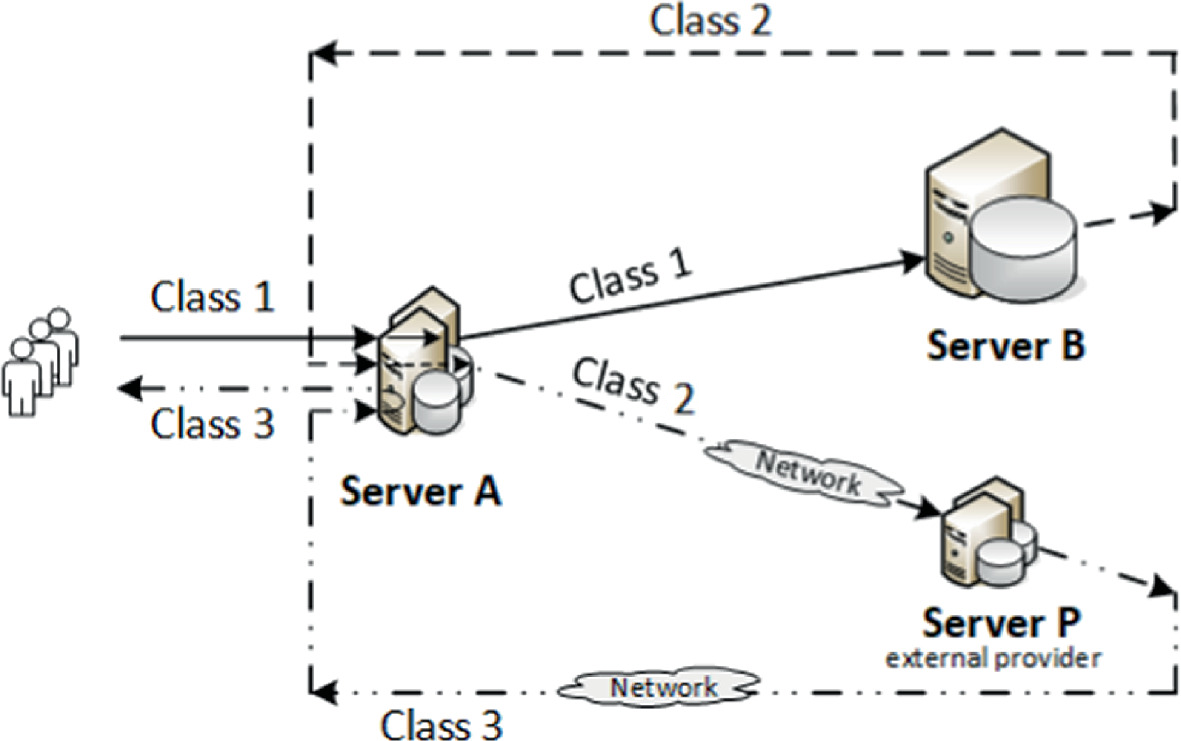
\includegraphics[width=0.8\linewidth]{figs/job_classes.png}
        \caption{Vista Bird-Eye dell'architettura distribuita della Web App. \citep{DBLP:books/sp/Serazzi24}}
        \label{fig:enter-label}
    \end{figure}
\end{frame}



\section{Metodologia}

\subsection{Obiettivi}
Procediamo con l'individuazione degli obiettivi della nostra analisi:
\begin{itemize}
    \item \textbf{Obiettivo 1}: ha lo scopo di implementare un modello in grado di rappresentare il sistema oggetto di studio e misurare tempo di risposta, popolazione e throughput medi. Tutte le metriche devono essere considerati sia locali, per singolo nodo, sia globalmente su tutto il sistema.
    \item \textbf{Obiettivo 2}: la WebApp decide di implementare un sistema di autenticazione a due fattori per rendere i pagamenti più sicuri. Ci siamo posti l'obiettivo di andare a valutare l'impatto di questa modifica sul sistema, valutando le stesse metriche dell'obiettivo precedente
    \item \textbf{Obiettivo 3}: vogliamo ora osservare il comportamento del sistema in caso di carico di richieste maggiore. Per i primi due obiettivi il massimo carico era di 4320 $job/h$ (ovvero 1.2 $job/s$) incrementato a circa 5000 $job/h$ (ovvero 1.4 $job/s$). Il confronto viene eseguito sulle stesse metriche dei primi due obiettivi.
    \item \textbf{Obiettivo 4}: l'ultimo obiettivo ha lo scopo di migliorare il sistema andando ad individuare eventuali bottleneck per migliorarne le prestazioni.
\end{itemize}

\subsection{Modello Concettuale}
Il sistema in analisi è stato modellato come una rete di code aperta il cui schema è riportato in \autoref{fig:queue_network_model}.\\
I job rappresentano gli utenti della WebApp dal momento in cui effettuano il login fino all'uscita successiva al checkout a seguito del pagamento.\\
Il percorso del job all'interno del sistema consiste in tre visite al centro A ed una visita ai centri B e P seguendo l'ordine: A-B-A-P-A. Dopo il terzo passaggio in A il job esce dal sistema. Per questo motivo è stata assegnata ai job una classe seguendo il seguente criterio:
\begin{itemize}
    \item \textbf{Classe 1}: sono i job che arrivano dall'esterno e restano in tale classe fino all'entrata in servizio in B.
    \item \textbf{Classe 2}: sono i job in arrivo nel server A tramite il feedback del server B e restano in tale classe fino all'entrata in servizio in P
    \item \textbf{Classe 3}: sono i job in arrivo nel server A tramite il feedback del server P. Sono anche la classe di job che escono dal sistema.
\end{itemize}
Con questa premessa le variabili di stato che meglio descrivono il sistema sono di due tipologie:
\begin{itemize}
    \item $N_{node,\ class}$: numero di job di classe $class \in \{1,2,3\}$ nel nodo $node \in \{A,B,P\}$
    \item $C_j\ con\ j \in [0, \infty)$: valore che indica la classe di appartenenza del job j.
\end{itemize}
La simulazione utilizzata è una \textit{next-event simulation}. Gli eventi sono di due tipologie, arrivi (Arrival) caratterizzati da server di destinazione e classe del job in arrivo e partenze (Departure) caratterizzato da server di partenza e classe del job in partenza. Non abbiamo inserito nessun evento artificiale\\
Di seguito l'evoluzione del sistema in base al verificarsi degli eventi divisi per server.\\
\textbf{Server A}
\begin{itemize}
    \item Arrivo dall'esterno del sistema: vengono modificate le variabile di stato incrementando $N_A,1$ e ponendo $C_j=1$. Vengono generati l'evento di Departure per il job di classe 1 dal server A e l'evento di arrival dall'esterno successivo;
    \item Departure di job di calsse 1: viene decrementata la variabile di stato $N_A,1$ e generato l'arrivo del job di classe 1 nel server B;
    \item Arrival di job di classe 2: viene incrementata la variabile di stato $N_A,2$, viene generato l'evento di Departure per il job di classe 2 dal server A.
    \item Departure di job di classe 2: viene decrementata la variabile di stato $N_A,2$. Viene generato l'arrivo del job di classe 2 nel server P;
    \item Arrival di job di classe 3: viene incrementata la variabile di stato $N_A,3$, viene generato l'evento di Departure per il job di classe 3 dal server A.
    \item Departure di job di classe 3: E' l'evento di uscita dal sistema. Viene decrementata la variabile di stato $N_A,3$.
\end{itemize}
\textbf{Server B}
\begin{itemize}
    \item Arrival di job di classe 1: viene incrementata la variabile di stato $N_B,1$, viene generato l'evento di Departure per il job di classe 1 dal server B.
    \item Departure di job di classe 1: vengono modificate le variabile di stato decrementando $N_B,1$ e ponendo $C_j=2$. Viene generato l'arrivo del job di classe 2 nel server A;
\end{itemize}
\textbf{Server P}
\begin{itemize}
    \item Arrival di job di classe 2: viene incrementata la variabile di stato $N_P,2$, viene generato l'evento di Departure per il job di classe 2 dal server P.
    \item Departure di job di classe 2: vengono modificate le variabile di stato decrementando $N_P,2$ e ponendo $C_j=3$. Viene generato l'arrivo del job di classe 3 nel server P;
\end{itemize}

\begin{figure}
    \centering
    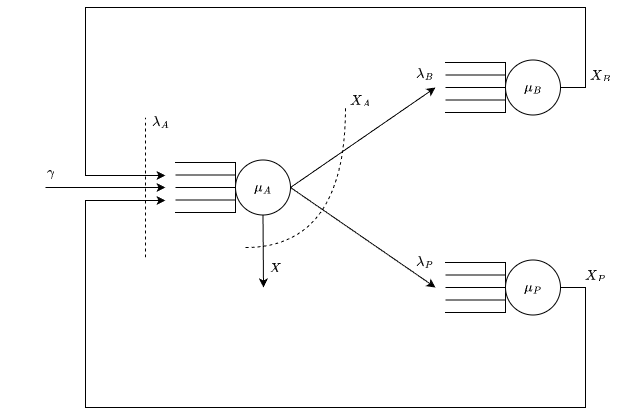
\includegraphics[width=\linewidth]{figs/webapp_conceptual.drawio.png}
    \caption{Diagramma del modello a reti di code del sistema}
    \label{fig:queue_network_model}
\end{figure}

\subsection{Modello delle Specifiche}
I valori di input, se non diversamente specificato, sono presi dal lavoro di \citet{DBLP:books/sp/Serazzi24}.

Le variabili indipendenti sono le seguenti:
\begin{itemize}
    \item Distribuzioni di probabilità dei servizi: Esponenziali;
    \item Distribuzioni di probabilità degli arrivi esterni: Esponenziali;
    \item Tempi di servizio medi per classe di job in ogni nodo: vedere \autoref{fig:average_service_per_job_class_by_node}
    \item Rate medi di arrivi esterni: valori che spaziano da $0.50$ a $1.20$ con un passo di $0.05 req/s$, per poi estendere fino a $1.40 req/s$ nel caso di carico pesante;
    \item Politiche di scheduling: PS per tutti i server coinvolti.
    \item Matrice di routing: consultando \autoref{fig:routing_matrix} e \autoref{fig:job_journey_with_classes} è possibile produrre la matrice di routing mostrata in \autoref{tab:routing-matrix}.
\end{itemize}

\begin{figure}
    \centering
    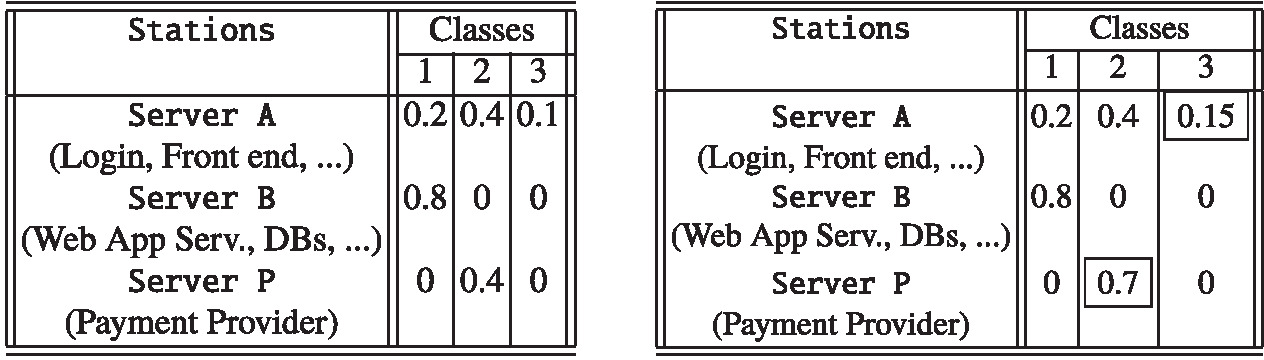
\includegraphics[width=1\linewidth]{figs/average_service_per_job_class_by_node.png}
    \caption{Tempi di servizio medi per classe di job in ogni nodo, nella versione vanilla (sinistra) e con 2FA (destra) \citep{DBLP:books/sp/Serazzi24}}
    \label{fig:average_service_per_job_class_by_node}
\end{figure}

\begin{figure}
    \centering
    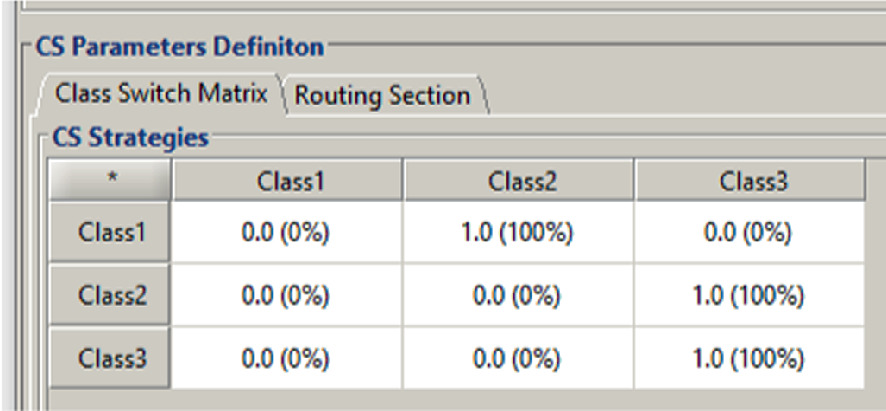
\includegraphics[width=1\linewidth]{figs/routing_matrix.png}
    \caption{Class switch matrix \citep{DBLP:books/sp/Serazzi24}}.
    \label{fig:routing_matrix}
\end{figure}

% Please add the following required packages to your document preamble:
% \usepackage{graphicx}
% \usepackage[table,xcdraw]{xcolor}
% Beamer presentation requires \usepackage{colortbl} instead of \usepackage[table,xcdraw]{xcolor}
\begin{table}[]
\centering
\caption{Routing Matrix per jobs di una certa classe che arrivano in un server. I valori nelle celle implicano una probabilità di routing pari a 1 verso i server specificati e 0 verso tutti gli altri. Il valore EXIT indica l'uscita dal sistema.}
\label{tab:routing-matrix}
\resizebox{\columnwidth}{!}{%
\begin{tabular}{
>{\columncolor[HTML]{FFFFFF}}l |
>{\columncolor[HTML]{FFFFFF}}l |
>{\columncolor[HTML]{FFFFFF}}l |
>{\columncolor[HTML]{FFFFFF}}l |}
\cline{2-4}
{\color[HTML]{222222} }                                                       & {\color[HTML]{222222} class 1}           & {\color[HTML]{222222} class 2}           & {\color[HTML]{222222} class3}        \\ \hline
\multicolumn{1}{|l|}{\cellcolor[HTML]{FFFFFF}{\color[HTML]{222222} Server A}} & {\color[HTML]{222222} \textbf{Server B}} & {\color[HTML]{222222} \textbf{Server P}} & {\color[HTML]{222222} \textbf{EXIT}} \\ \hline
\multicolumn{1}{|l|}{\cellcolor[HTML]{FFFFFF}{\color[HTML]{222222} Server B}} & {\color[HTML]{222222} \textbf{Server A}} & {\color[HTML]{222222} }                  & {\color[HTML]{222222} }              \\ \hline
\multicolumn{1}{|l|}{\cellcolor[HTML]{FFFFFF}{\color[HTML]{222222} Server P}} & {\color[HTML]{222222} }                  & {\color[HTML]{222222} \textbf{Server A}} & {\color[HTML]{222222} }              \\ \hline
\end{tabular}%
}
\end{table}

Le variabili dipendenti sono le seguenti metriche di performance:
\begin{itemize}
    \item Tempo di risposta $T$: detto anche Tempo di Residenza, è l'intervallo di tempo che una richiesta trascorre all'interno di un nodo (o del Sistema) dal momento in cui entra fino al momento in cui esce;
    \item Popolazione $N$: numero di richieste all'interno di un nodo (o nel Sistema);
    \item Throughput $X$: numero di richieste soddisfatte sull'unità di tempo da un nodo (o dal Sistema). 
    \item Utilizzazione $\rho$: proporzione di tempo in cui il nodo è occupato dall'esecuzione delle richieste.
\end{itemize}

\subsection{Modello Computazionale}
Il codice del simulatore è stato realizzato in Python ed è disponibile al seguente indirizzo: \url{https://github.com/caballo-domestico/webapp-workflow-pa}

\subsubsection{Scheduler Next-Event}
\autoref{fig:scheduler_nextevent_class_diagram} illustra l'architettura dello scheduler Next-Event. Per implementare una Next-Event simulation è stato definito un oggetto \texttt{NextEventScheduler}, che mantiene una event list, ovvero una lista di oggetti \texttt{Event} ordinata secondo il tempo di schedulazione. È possibile aggiungere un evento allo scheduler attraverso il metodo \texttt{schedule(event, delay)}, il quale verrà inserito alla posizione corrispondente al suo tempo di schedulazione, con l'aggiunta di un delay opzionale. È inoltre possibile annullare la schedulazione di un evento attraverso il metodo \texttt{cancel(event)}, che dunque non verrà più processato pur rimanendo nella event list. Lo scheduler espone un'interfaccia da iteratore, ovvero attraverso i metodi \texttt{has\_next()} e \texttt{next()} è possibile consumare gli eventi della event list, ovvero processarli. Per processare un evento, ne viene invocato l'\texttt{EventHandler} corrispondente che ne implementa i dovuti cambiamenti di stato.

\begin{figure}
    \centering
    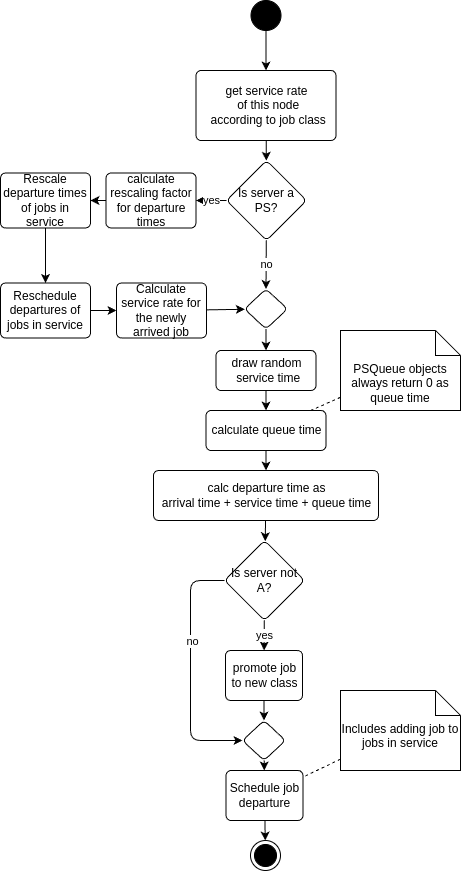
\includegraphics[width=1\linewidth]{figs/diagrams/handle_arrival.drawio.png}
    \caption{Activity diagram dell'handler degli arrivi.}
    \label{fig:handle_arrival}
\end{figure}

\subsubsection{Arrivi e Partenze dei jobs}
\autoref{fig:handle_arrival} mostra i passaggi da intraprendere per gestire l'evento di arrivo di un job a un nodo. In sintesi, l'handler calcola il tempo di departure del nodo come la somma dei seguenti tempi:
\begin{itemize}
    \item Arrival time: tempo di simulazione all'istante di arrivo del nodo;
    \item Service time: tempo che il job deve spendere in servitura, estratto casualmente dalla distrubuzione dei servizi del nodo con parametri che dipendono dalla classe del job;
    \item Queue time: tempo che il job spende nella coda del nodo, che dipende dalla politica di scheduling e dai jobs residenti nel nodo.
\end{itemize}
Nel caso in cui la politica di scheduling sia PS è necessaria particolare attenzione, infatti il ricambio di jobs residenti nel nodo implica un aggiornamento dei tempi di servizio dei jobs già in servitura. Se chiamiamo $S_{rem}$ il tempo di servizio rimanente per un certo job con $N$ jobs in servitura nel nodo otteniamo \autoref{eq:s_rem_ps}, dove $D_{rem}$ è la domanda rimanente da smaltire per completare il servizio su quel job.
\begin{equation}
  \begin{aligned}
    S_{rem} = \frac{D_{rem}}{\frac{\mu}{N}}
  \end{aligned}
  \label{eq:s_rem_ps}
\end{equation}
Nel momento in cui arriva un nuovo job nel nodo, il suo tempo rimanente andrebbe ora calcolato come in \autoref{eq:s_rem_star_ps}, dove $N^*$ è il nuovo numero di jobs nel nodo che include il nuovo job arrivato.
\begin{equation}
  \begin{aligned}
    S^*_{rem} = \frac{D_{rem}}{\frac{\mu}{N^*}}
  \end{aligned}
  \label{eq:s_rem_star_ps}
\end{equation}
Si noti come $D_{rem}$ sia ovviamente la stessa quantità sia in \autoref{eq:s_rem_ps} che in \autoref{eq:s_rem_star_ps}. Mettendo a sistema le due equazioni otteniamo \autoref{eq:s_rem_star_final_ps}, dove $\frac{N^*}{N}$ è il Rescaling Factor menzionato in \autoref{fig:handle_arrival}.
\begin{equation}
  \begin{aligned}
    S^*_{rem} = S_{rem} \frac{N^*}{N}
  \end{aligned}
  \label{eq:s_rem_star_final_ps}
\end{equation}
Usando \autoref{eq:s_rem_star_final_ps} è possibile aggiornare i tempi delle partenze dei job già in servizio nel nodo nel momento in cui arriva un nuovo job. L'effetto che si ottiene è che con l'arrivo di nuovi job, i tempi di servizio rimanente si allungano. Nel caso particolare in cui il job arrivi in un nodo vuoto, allora sia $N$ che $N^*$ sono pari a 1.

\autoref{fig:handle_departure} mostra l'Activity Diagram dell'handler che gestisce la partenza di un job da un nodo. Essenzialmente, rimuove il job dall'insieme dei job residenti al nodo in questione, e se necessario genera un nuovo evento di arrivo al nodo di destinazione. Se il nodo ha politica PS è necessario aggiornare le departures dei nodi ancora residenti usando sempre \autoref{eq:s_rem_star_final_ps}, con l'effetto di accorciare i tempi di servizio rimanenti.

\begin{figure}
    \centering
    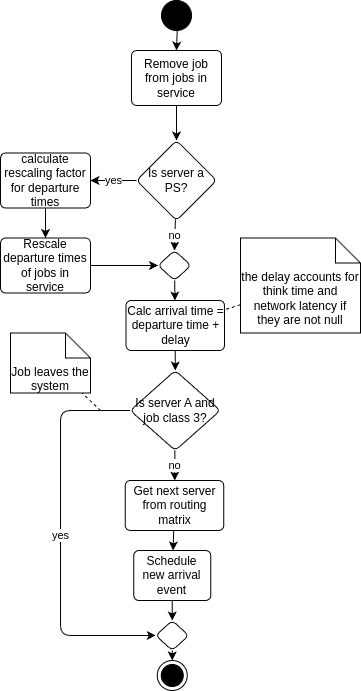
\includegraphics[width=1\linewidth]{figs/diagrams/handle_departure.drawio.png}
    \caption{Activity diagram dell'handler delle partenze.}
    \label{fig:handle_departure}
\end{figure}

\subsubsection{Event-Oriented Programming}
È possibile iscrivere degli \\ \texttt{EventHandler} alla ricezione di uno o più tipi di eventi poiché lo scheduler implementa un pattern Pub-Sub push-notify. L'iscrizione agli eventi può avvenire attraverso i seguenti metodi dello scheduler:
\begin{itemize}
    \item \texttt{subscribe(event\_type, event\_handler)}: l'\texttt{EventHandler} viene invocato dopo che l'evento è stato elaborato, ovvero il suo handler ha terminato l'esecuzione;
    \item \texttt{intercept(event\_type, event\_handler)}: l'\texttt{EventHandler} viene invocato prima che l'evento è stato elaborato, e può modificare l'\texttt{Event} stesso.
\end{itemize}
Non c'è garanzia sull'ordine della ricezione delle notifiche tra subscribers e tra interceptors. Inoltre, iscriversi a un tipo di \texttt{Event} comporta la ricezione delle notifiche anche per eventi che specializzano quel tipo di eventi. Ad esempio, iscriversi al tipo \texttt{Event} implica la ricezione di una notifica ad ogni evento processato. Gli eventi annullati non comportano l'invio di notifiche.

A supporto della realizzazione delle simulazioni sono stati implementati i seguenti subscribers e interceptors:
\begin{itemize}
    \item \texttt{BatchMeansInterceptor}: Intercetta eventi di arrivi esterni per tenerne il conto. Se il conteggio supera il numero di arrivi previsto per il batch, salva le statistiche finora calcolate per questo batch e ripristina le statistiche cacolate dagli stimatori per il prossimo batch.
    \item \texttt{ArrivalsGeneratorSubscriber}: Si mette in ascolto di arrivi esterni e ne tiene il conto. Per ogni arrivo ricevuto, schedula un nuovo arrivo esterno dopo un tempo di interarrivo casuale, fino a quando gli arrivi contati superano il numero massimo di arrivi previsto.
\end{itemize}

\subsubsection{Misurazione metriche di performance}
Gli stimatori delle misurazioni delle metriche di performance sono stati implementati come subscribers e sono i seguenti:
\begin{itemize}
    \item \texttt{BusytimeEstimator}: Si mette in ascolto di arrivi e partenze dei job. Per ogni nodo, traccia gli arrivi e le partenze e tiene conto del numero di jobs ancora presenti nel nodo. Se a causa di un arrivo tale numero passa da zero a maggiore di zero, l'istante di tempo di tale arrivo segna l'inizio di un busy period per quel nodo, che terminerà solo quando tale numero scende di nuovo a zero, oppure lo stimatore è resettato (i.e. quando cambia il batch);
    \item \texttt{ObservationTimeEstimator}: Si iscrive a tutti gli eventi e tiene il conto del tempo di simulazione trascorso dalla sua iscrizione o dal suo ultimo reset;
    \item \texttt{CompletionsEstimator}: Si iscrive alle partenze dei jobs dai nodi. Per ogni nodo,
    conta il numero di partenze dall'inizio della simulazione o dal reset dello stimatore;
    \item \texttt{ResponseTimeEstimator}: Si iscrive agli arrivi e alle partenze dei jobs. Per ogni nodo, si segna il tempo di arrivo e di partenza di ogni job e ne calcola il tempo di risposta come la differenza dei due valori.
    \item \texttt{PopulationEstimator}: Si iscrive agli arrivi e alle partenze dei jobs. Per ogni nodo, ne incrementa il conteggio della popolazione dei jobs per ogni arrivo ricevuto e la decrementa per ogni partenza.
\end{itemize}

Gli stimatori \texttt{ResponseTimeEstimator} e \texttt{PopulationEstimator} mantengono una media dei valori campionati usando un oggetto \texttt{WelfordEstimator}, che implementa l'algoritmo di Welford per il calcolo online della media \citep{des}. Inoltre, tale oggetto calcola anche la Standard Deviation, il Min value e il Max value dei campioni raccolti durante una run. Gli altri stimatori mantengono invece la somma dei campioni.

\begin{figure*}
    \centering
    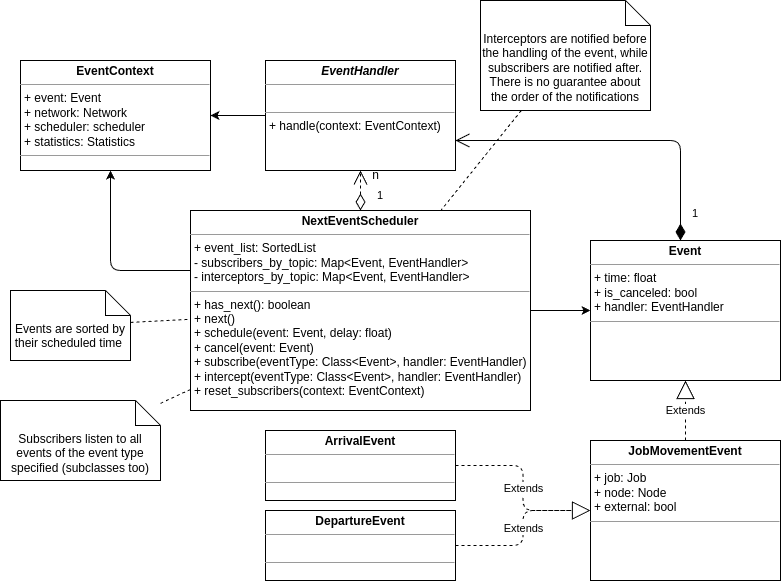
\includegraphics[width=\linewidth]{figs/diagrams/scheduler.drawio.png}
    \caption{Vista delle classi che implementano uno scheduler Next-Event.}
    \label{fig:scheduler_nextevent_class_diagram}
\end{figure*}

\subsubsection{Modello}
\autoref{fig:simulation_class_diagram} mostra come il modello a rete di code è implementato nel sistema. Un oggetto \texttt{Network} si compone di diversi \texttt{Node}, ognuno dei quali è composto da un \texttt{Server} e da una \texttt{Queue}. Il \texttt{Server} implementa il servente e attraverso il metodo \texttt{get\_service(service\_rate)} genera un tempo di servizio casuale secondo un certo rate e distribuzione di probabilità, dopo aver selezionato lo stream corretto. La \texttt{Queue} calcola il tempo che un job deve spendere in coda prima che sia il suo turno di essere servito in base alla politica di scheduling. I tempi di interrarrivo esterni sono calcolati dalla \texttt{Network} secondo la sua distribuzione di probabilità degli arrivi e il rate medio di arrivi.

\subsubsection{Processi stocastici}
La simulazione dei processi casuali è stata implementata usando il modulo \texttt{rngs} \citep{des}, il quale mette a disposizione diversi streams di generatori di Lehmer in grado di produrre una sequenza di numeri pseudo-casuali secondo una distribuzione desiderata. Per ogni processo casuale indipendente simulato nel sistema è selezionato uno stream dedicato, ovvero si imposta il seed del generatore al valore corrente per quello stream prima di pescare il prossimo numero della sequenza. I processi pseudo-casuali indipendenti implementati nel sistema sono:
\begin{itemize}
    \item Gli arrivi dall'esterno del sistema al server A;
    \item I servizi del server A;
    \item I servizi del server B;
    \item I servizi del server P;
\end{itemize}

\begin{figure*}
    \centering
    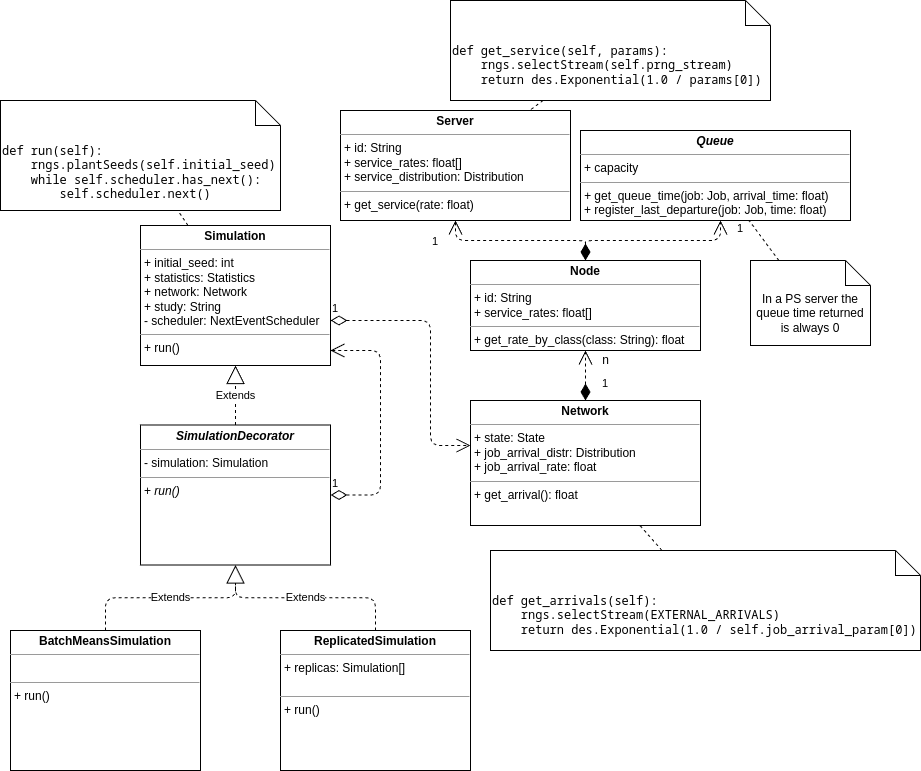
\includegraphics[width=\linewidth]{figs/diagrams/simulation.drawio.png}
    \caption{Vista delle classi che implementano una Simulazione.}
    \label{fig:simulation_class_diagram}
\end{figure*}

\subsubsection{Simulation Runs}
Una simulazione è implementata come un oggetto \texttt{Simulation}, come illustrato in \autoref{fig:simulation_class_diagram}. Attraverso l'uso di decoratori, sono state implementate due varianti di simulazione:
\begin{itemize}
    \item \texttt{BatchMeansSimulation}: Iscrive alla simulazione decorata un \texttt{BatchMeansInterceptor} per implementare una simulazione Batch Means;
    \item \texttt{ReplicatedSimulation}: Decora una sequenza di simulazioni identiche e le esegue in sequenza, impostando il seed iniziale della prossima replica come l'ultimo valore della sequenza prng (\texttt{DEFAULT} stream) generato dalla replica precedente.
\end{itemize}
È possibile implementare una run di simulazione aggiungendo a runtime i comportamenti desiderati utilizzando opportunatamente decoratori, subscribers e interceptors, oltre a costruire la rete di code desiderata andando a comporre opportunamente oggetti \texttt{Server} e \texttt{Queue} in oggetti \texttt{Node}, e questi ultimi in una \texttt{Network} da associare poi alla \texttt{Simulation}. Inoltre, è necessario impostare un evento iniziale che di fatto dà il via alla simulazione. Nel nostro caso, abbiamo delegato la complessità della costruzione di una simulazione in una \texttt{SimulationFactory}. Queste caratteristiche rendono il simulatore molto potente e flessibile in termini di features mantenendone contenuta la complessità della implementazione.   

Una volta costruita una \texttt{Simulation}, per eseguirla è sufficiente invocarne il metodo \texttt{run()}, che imposta il seed iniziale per i vari streams del prng e avvia la consumazione degli eventi. Quando non ci sono più eventi da consumare, la simulazione termina e viene effettuato il salvataggio delle statistiche su dei file \texttt{.csv} nella cartella \texttt{statistics}. I parametri della simulazione sono definiti in un file \texttt{config.json}, dove a ogni entry corrisponde un set di valori di parametri che realizzano un Simulation Study.


\subsection{Verifica}
Per la verifica della correttezza del simulatore abbiamo studiato il modello analitico del sistema. Il tale modello però non può tenere conto delle tre classi servite dal server A che richiederebbero tre tassi di servizio differenti.\\
Abbiamo osservato che nel server A entrano tre flussi di job: uno per gli arrivi dall'esterno, due dai feedback dei server B e P. Essendo il percorso dei job deterministico abbiamo concluso che la probabilità di trovare un job di una specifica classe in servizio nel server A è uguale ad $\frac{1}{3}$ per ogni classe. Abbiamo quindi trattato tutti i job del server A con un rate ottenuto facendo la media delle tre classi:
\begin{equation}
\displaystyle {\mu}_{A} = \sum_{c=1}^{3} {\mu}_{A,c} {p}_{A,c}
\end{equation}
Dove ${\mu}_{A,c}$ è il tasso di servizio della classe \textit{c} nel server A e ${p}_{A,c}$ è la probabilità di trovare un job di classe \textit{c} nel server A se quest'ultimo è occupato.
Considerato quanto detto fin'ora e con l'ulteriore assunzione che il flusso dei job è bilanciato possiamo scrivere \autoref{eq:lambdas} che esprime i rate di arrivi a ogni server, calcolati risolvendo il bilanciamento dei flussi riportato in \autoref{eq:flow-balance} e ottenendo cosi \autoref{eq:flow-balance-solved}.

\begin{equation}
  \begin{aligned}
    & \displaystyle {\lambda}_{A} = \gamma + {X}_{B} + {X}_{P}\\
    & \displaystyle {\lambda}_{B} = {X}_{B}\\
    & \displaystyle {\lambda}_{P} = {X}_{P}
  \end{aligned}
  \label{eq:lambdas}
\end{equation}

\begin{equation}
  \left\{\begin{array}{@{}l@{}}
    \displaystyle \gamma + {X}_{B} + {X}_{P} = \left({p}_{A,1} + {p}_{A,2} + {p}_{A,3}\right) {X}_{A}\\
    \displaystyle {X}_{A} {p}_{A,1} = {X}_{B}\\
    \displaystyle {X}_{A} {p}_{P,2} = {X}_{P}
  \end{array}\right.\
  \label{eq:flow-balance}
\end{equation}

\begin{equation}
  \begin{aligned}
    & \displaystyle {X}_{A} = {\lambda}_{A} = 3\gamma\\
    & \displaystyle {X}_{B} = {\lambda}_{B} = \gamma\\
    & \displaystyle {X}_{P} = {\lambda}_{P} = \gamma
  \end{aligned}
  \label{eq:flow-balance-solved}
\end{equation}
Per ogni obiettivo prima di procedere al calcolo degli indici locali e globali andiamo a calcolare l'utilizzazione al variare del tasso di arrivo dall'esterno $\gamma$ per ogni server per assicurarci che siano stabili.
\begin{equation}
\displaystyle {\rho}_{s} = \frac{{\lambda}_{s}}{\mu_{s}}
\end{equation}
Per il calcolo del tempo di risposta per ogni server abbiamo utilizzato \autoref{eq:ps-rtime}.
\begin{equation}
\displaystyle {E[T]}_{s} = \frac{1}{\left(1 - {\rho}_{s}\right) {\mu}_{s}}
\label{eq:ps-rtime}
\end{equation}
Mentre per la popolazione media abbiamo utilizzato la legge di Little riportata in \autoref{eq:little}.
\begin{equation}
    \displaystyle {E[N]}_{s} = {E[T]}_{s} {\lambda}_{s}
    \label{eq:little}
\end{equation}
Infine per quanto riguarda gli indici globali sono stati calcolati come in \autoref{eq:output-global}. Abbiamo calcolato per ogni nodo le visite medie con l'\autoref{eq:visits}. Con le visite medie abbiamo potuto calcolare il tempo di risposta medio e, di conseguenza, utilizzando il teorema di Little la popolazione media. Per quanto riguarda il throughput viene preso in considerazione quello del server A dei soli job di classe 3 ovvero quelli che escono dal sistema. Essendo dipendente dal tasso di arrivo $\gamma$ ciò è valido solo se il sistema è stabile.
\begin{equation}
    \displaystyle {v}_{s} = \frac{{\lambda}_{s}}{\gamma}
    \label{eq:visits}
\end{equation}
\begin{equation}
  \begin{aligned}
    & \displaystyle E[T] = \sum_{s=A}^{P} {E[T]}_{s} {v}_{s}\\
    & \displaystyle E[N] = \gamma E[T]\\
    & \displaystyle X = {X}_{A} {p}_{A,3}
  \end{aligned}
  \label{eq:output-global}
\end{equation}



\subsection{Validazione}
In assenza di dati sperimentali riguardanti una implementazione reale della Web App non è possibile effettuare una validazione vera e propria. Tuttavia, assumendo che il simulatore descritto da \citet{DBLP:books/sp/Serazzi24} sia stato validato su un caso di studio reale, abbiamo validato i nostri risultati con quelli della fonte citata.

\subsection{Simulation Studies}
Gli obiettivi che ci siamo posti ci hanno portato ad eseguire diverse run con configurazioni diverse di parametri. Per ogni obiettivo viene eseguita una run per ogni tasso di arrivo. Le run effettuate sono simulazioni ad orizzonte infinito implementate come Batch-Means, con 100 batch da 64 job ognuno.\\
\begin{itemize}
    \item \textbf{Obiettivo 1}: nel primo esperimento consideriamo i server nel loro assetto base con rate di servizio elencati in \autoref{tab:service-rates-vanilla}.
    Inoltre solo per questo obiettivo abbiamo voluto osservare il comportamento dello stato transitorio effettuando anche una replicated simulation di 100 repliche da 64 job ciascuna in modo simmetrico rispetto alla simulazione batch means.
    \item \textbf{Obiettivo 2}: in questo caso i server subiscono una diminuzione dei rate di servizio a causa dell'autenticazione a due fattori. Per il server A nel caso di job di classe 3, diventa 6.6667$job/s$, mente per il server P diventa 1.4285$job/s$, resta invariato per B.
    \item \textbf{Obiettivo 3}: in questo caso abbiamo esteso i tassi di arrivo fino al nuovo carico pesante richiesto, mentre per i tassi di servizio si torna alla configurazione base dei server.
    \item \textbf{Obiettivo 4}: per questo obiettivo, come approfondiremo più avanti, sono state fatte più run al variare del rate di servizio del server B nel tentativo di migliorare le performance del sistema. Gli altri server hanno mantenuto la loro configurazione base.
\end{itemize}
\begin{table}
    \centering
    \caption{Tassi di servizio medi per classe di job offerti da ogni nodo.}
    \begin{tabular}{ccccc}
         & Classe 1 & Classe 2 & Classe 3 \\
         Server A & 5 & 2.5 & 10\\
         Server B & 1.25 & 0 & 0\\
         Server C & 0 & 2.5 & 0\\
    \end{tabular}
    \label{tab:service-rates-vanilla}
\end{table}
Per ogni obiettivo abbiamo generato i seguenti grafici per ogni metrica (tempo medio di risposta, popolazione media, throughput, utilizzazione), per ogni nodo e globalmente per il sistema:

Per ogni run differente viene fatta la media dei valori medi delle metriche in modo da aggregare i dati ottenuti intra-run (le medie delle metriche per singolo batch nel caso di simulazione ad orizzonte infinito e della singola replica per l'orizzonte finito). Allo stesso modo viene calcolata la deviazione standard ed il numero di sample points. Abbiamo quindi calcolato l'intervallo di confidenza secondo \autoref{eq:confidence-interval}:
\begin{equation}
    CI = \bar{x} \pm z \cdot \frac{\sigma}{\sqrt{n}}
    \label{eq:confidence-interval}
\end{equation}
Dove $\bar{x}$ è la media campionaria, $z$ è il valore critico della distribuzione normale sandard considerato a livello di confidenza del 95\% (ha valore 1.96), $\sigma$ è la deviazione standard ed $n$ il numero di sample points.\\
Inoltre abbiamo utilizzato i valori delle metriche ottenuti per batch (o per replica) per osservare la loro distribuzione.

\section{Risultati e Discussione}
I valori grezzi delle  misurazioni sperimentali sono disponibili a \url{https://github.com/caballo-domestico/webapp-workflow-pa/raw/refs/heads/main/docs/replication_data_kit/statistics.zip}. I dati in forma tabellare del modello analitico sono disponibili a \url{https://github.com/caballo-domestico/webapp-workflow-pa/blob/main/docs/model/classless.ipynb}, mentre i risultati elaborati di questo studio sono disponibili a \url{https://github.com/caballo-domestico/webapp-workflow-pa/blob/main/docs/plots/model_plots.ipynb}.\\

\subsection{Obiettivo 1}
\subsubsection{Risultati sperimentali}
In \autoref{fig:obj1_boxplot_utilization} andiamo ad analizzare il comportamento dell'utilizzazione. Per tutti i nodi l'andamento è crescente, come ci aspettavamo, la dispersione è piuttosto simile tra i vari box ad eccezione del server B con tasso di arrivo 1.2$job/s$, in questo caso il box è schiacciato verso 1. Sia il server A che il server B presentano valori di massimo che raggiungono 1, invece per quanto riguarda i valori medi di utilizzazione il valore più alto che troviamo è di 0.97 per il server B quando il tasso di arrivo è 1.2$job/s$, seguito dal caso con tasso di arrivo 1.15$job/s$ ed utilizzazione 0.92 sempre per il server B. Per i valori medi sono gli unici due casi che superano lo 0.9.\\
Da notare anche come le performance del server B influenzino l'andamento del sistema.
\begin{figure*}
    \centering
    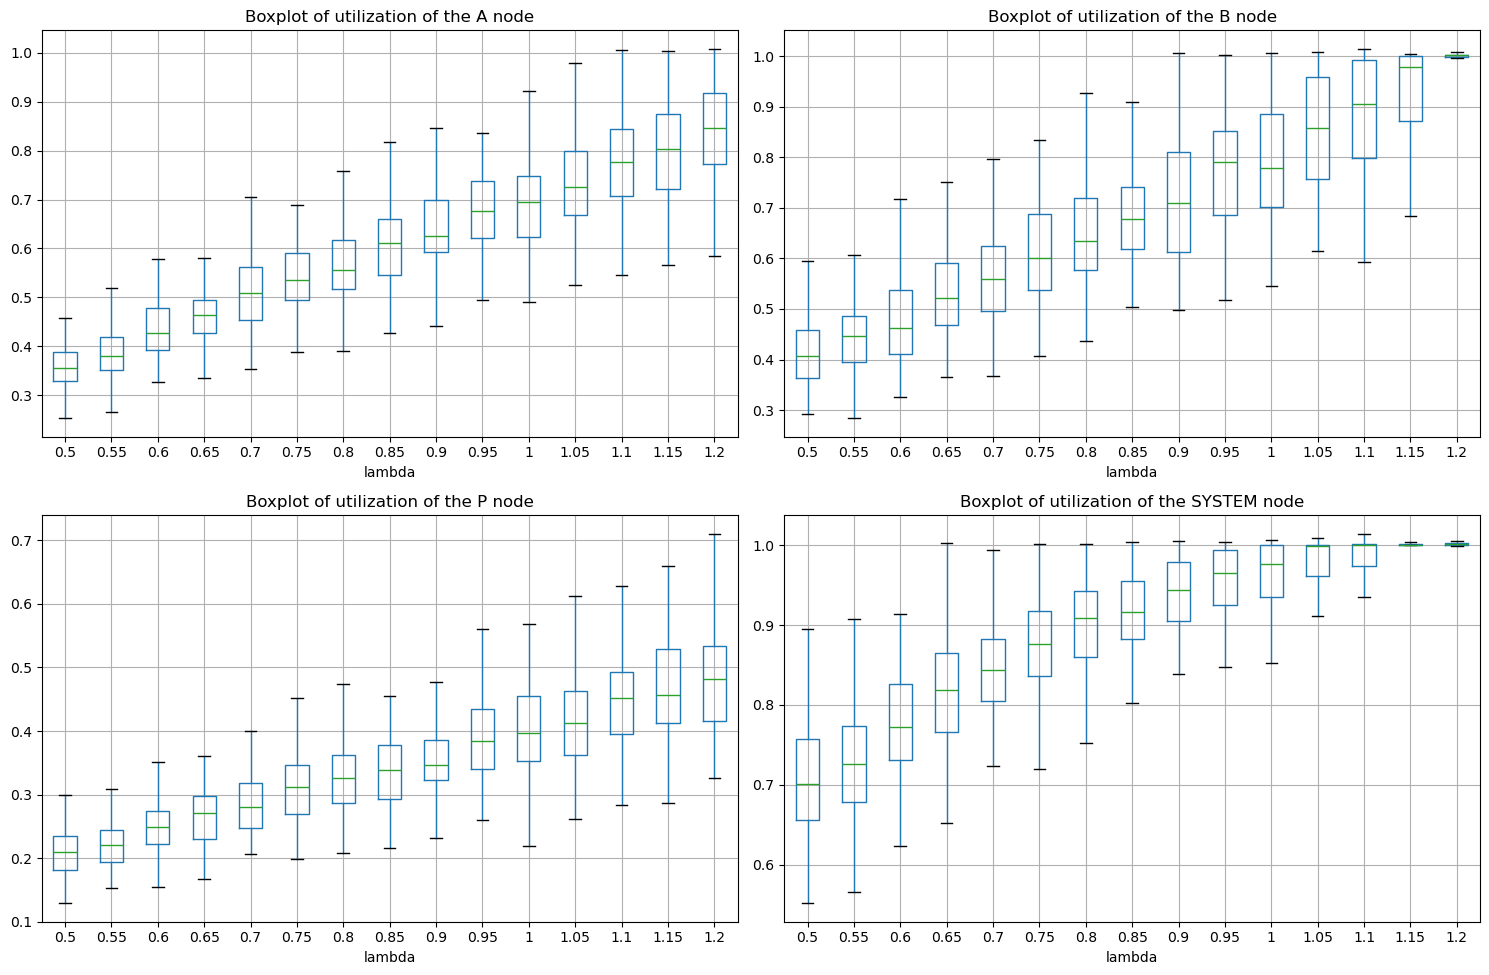
\includegraphics[width=\textwidth]{figs//results/obj1/obj1-box-utilization.png}
    \caption{Distribuzione dell'utilizzazione dei risultati sperimentali dell'obbiettivo 1.}
    \label{fig:obj1_boxplot_utilization}
\end{figure*}
Per quanto riguarda la popolazione media in \autoref{fig:obj1_boxplot_population} il server P riesce a mantenere dei valori in un range abbastanza ristretto, non superando mai l'1.5$job$ di media, rispetto al server A che presenta un andamento costantemente crescente fino ad arrivare a 5.78$job$. Per quanto riguarda il server B presenta un andamento costantemente crescente fino al rate di arrivi 1.1$job/s$, mentre per gli ultimi due valori (1.15$job/s$ e 1.12$job/s$) presenta dei picchi di 11$job$ e 31$job$, comportamento atteso visto il valore prossimo all'1 dell'utilizzazione.
\begin{figure*}
    \centering
    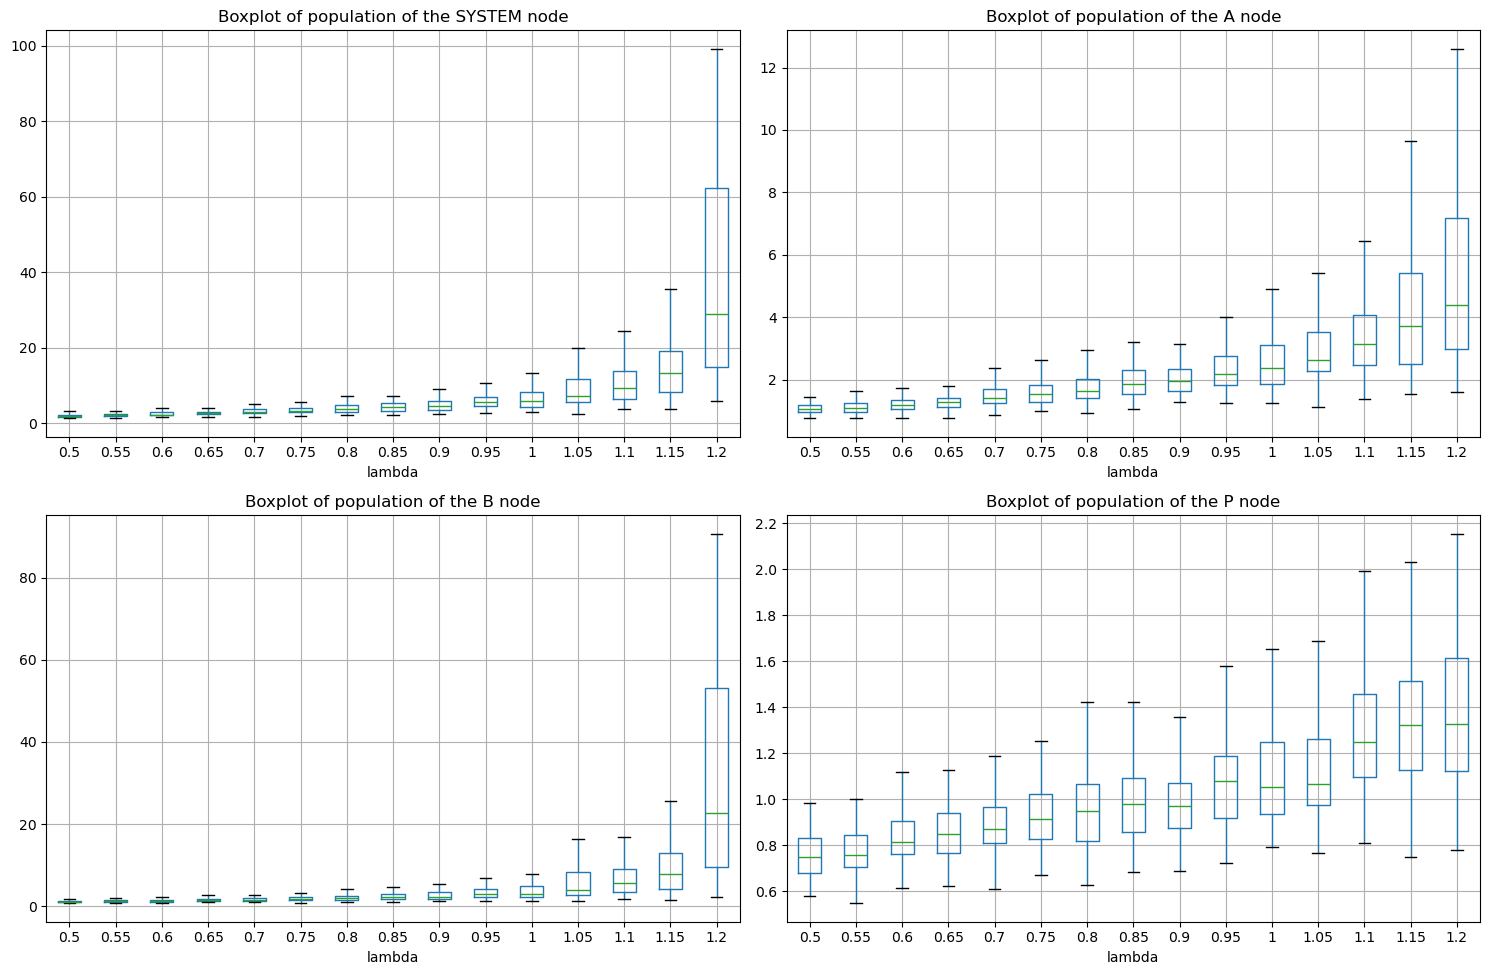
\includegraphics[width=\textwidth]{figs//results/obj1/obj1-box-population.png}
    \caption{Distribuzione della popolazione media dei risultati sperimentali dell'obbiettivo 1.}
    \label{fig:obj1_boxplot_population}
\end{figure*}
Comportamento analogo segue il tempo medio di risposta in \autoref{fig:obj1_boxplot_response_time}, il server P presenta come valore medio massimo 0.78$s$ in corrispondenza del tasso di arrivo massimo, mentre il server A arriva a 1.47$s$. Il server B è in un range più ampio con picchi, per i tassi di arrivo 1.15$job/s$ e 1.2$job/s$, che arrivano a 9.38$s$ e 25.50$s$.
\begin{figure*}
    \centering
    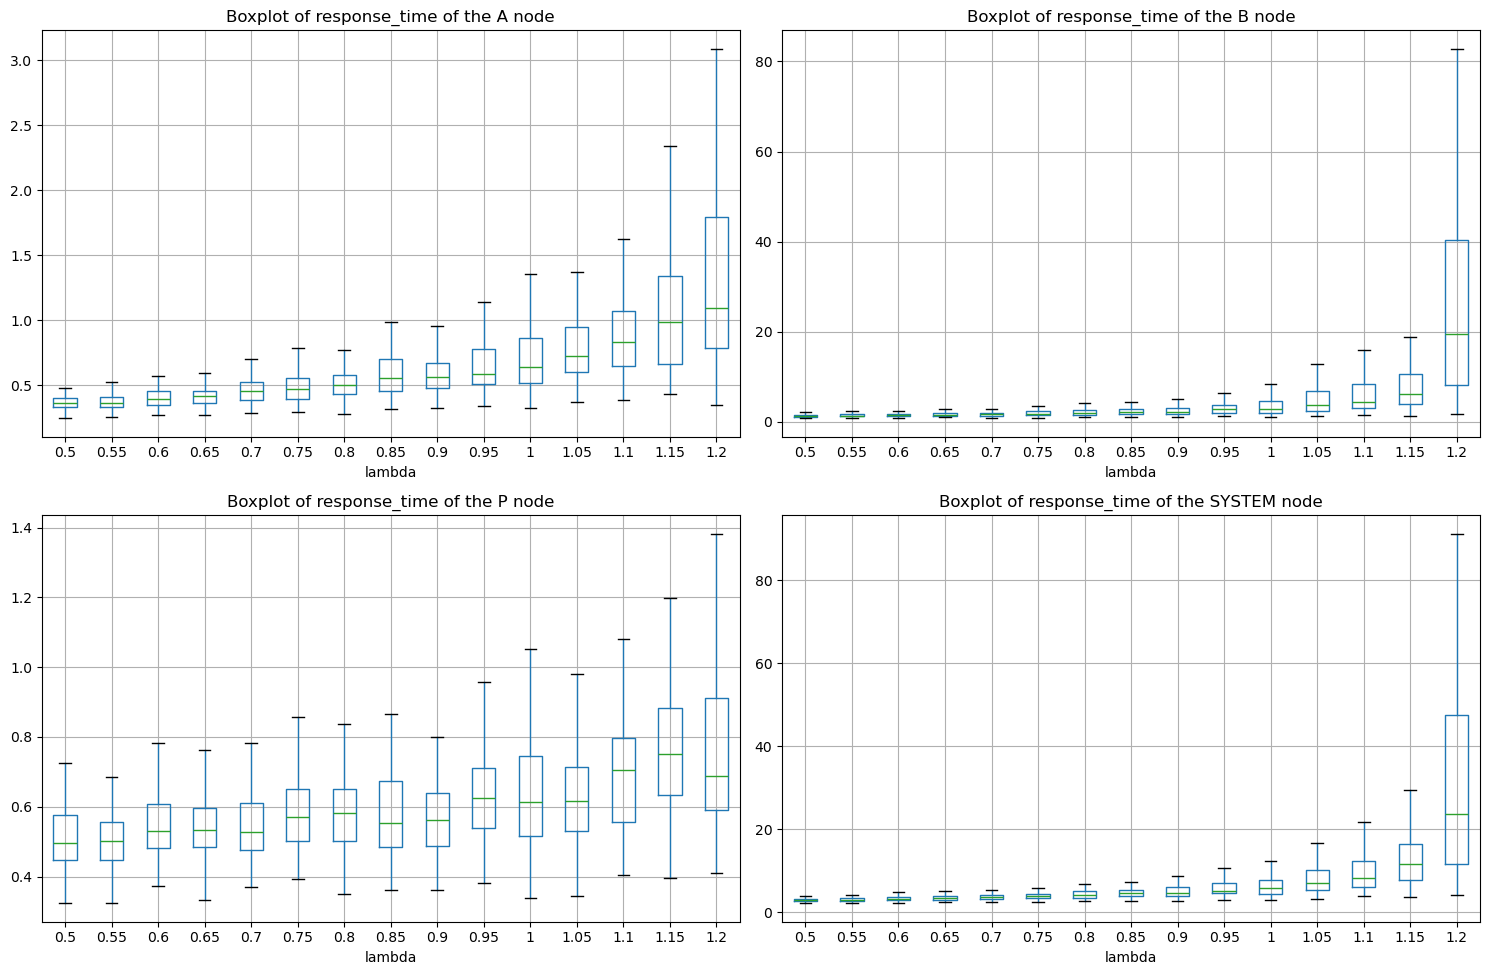
\includegraphics[width=\textwidth]{figs//results/obj1/obj1-box-response-time.png}
    \caption{Distribuzione dei tempi di risposta medi dei risultati sperimentali dell'obbiettivo 1.}
    \label{fig:obj1_boxplot_response_time}
\end{figure*}
Infine per il throughput in \autoref{fig:obj1_boxplot_throughput} tutti e tre i server hanno un andamento costantemente crescente, indice che comunque riescono a servire i job in arrivo. Il server A ha il throughput più alto, mentre B e P hanno un andamento molto simile come si può vedere anche dal grafico in \autoref{fig:obj1_throughput_comparison}

\begin{figure}[H]
    \centering
    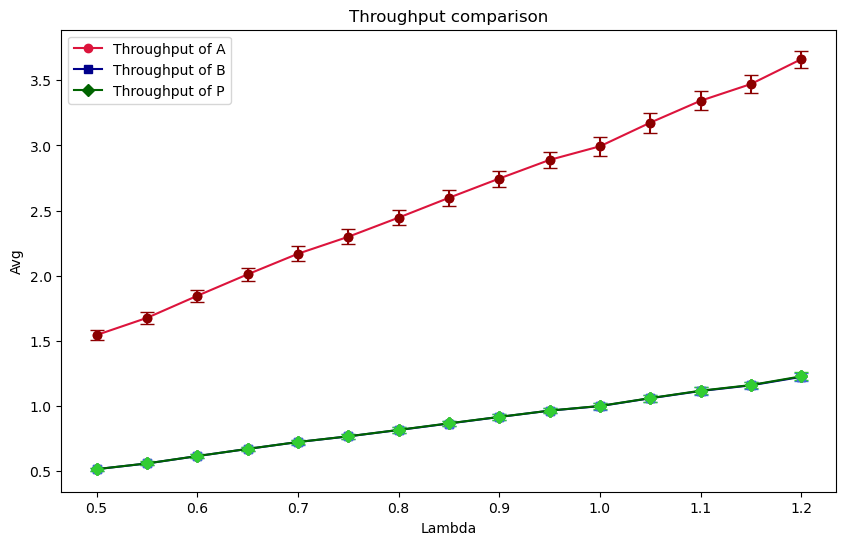
\includegraphics[width=\columnwidth]{figs/results/obj1/obj1-throughput-comparison.png}
    \caption{Confronto throughput per i server A, B e P per l'obiettivo 1}
    \label{fig:obj1_throughput_comparison}
\end{figure}

\begin{figure*}
    \centering
    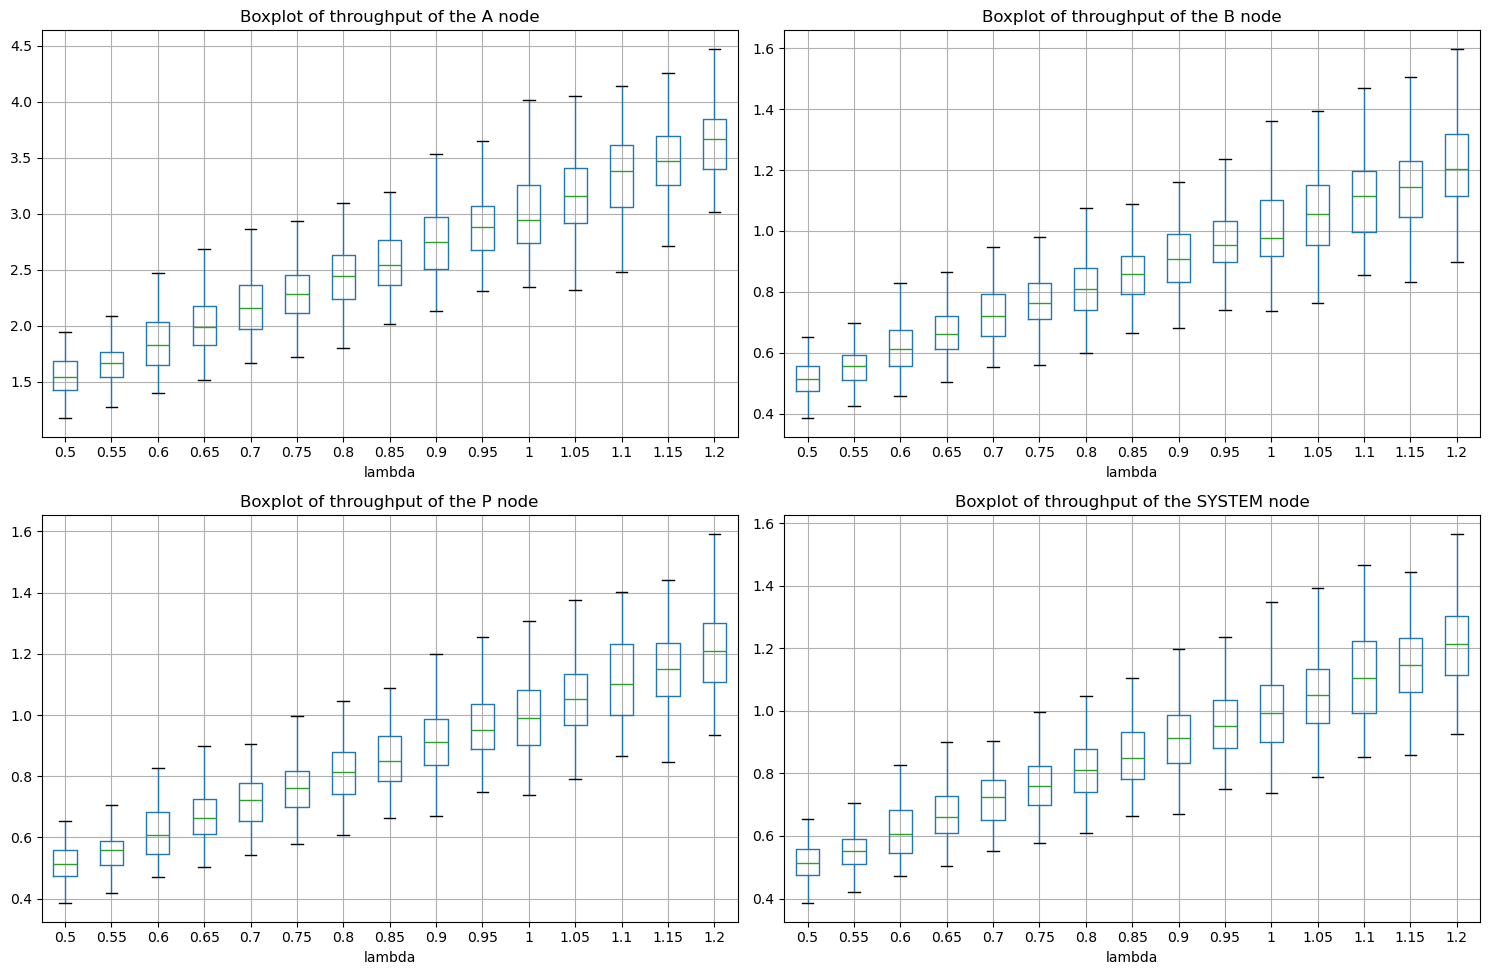
\includegraphics[width=\textwidth]{figs//results/obj1/obj1-box-throughput.png}
    \caption{Distribuzione del throughput medio dei risultati sperimentali dell'obbiettivo 1.}
    \label{fig:obj1_boxplot_throughput}
\end{figure*}


\subsubsection{Verifica con il modello analitico}
Per il tasso di servizio del server A nel modello analitico abbiamo utilizzato i seguenti parametri:
$\displaystyle {\mu}_{A} = 5.833 job/s$.
Mentre i tassi di servizio per i server B e P restano invariati rispetto alla simulazione: $\displaystyle {\mu}_{B} = 1.25job/s$ e $\displaystyle {\mu}_{P} = 2.5job/s$.\\
Per ogni lambda i nodi risultano stabili, riportiamo i valori per tasso di arrivo minimo e massimo:

\begin{table}[!htbp]
    \centering
    \begin{tabular}{cccc}
         $\gamma$ & $\rho_{A}$ & $\rho_{B}$ & $\rho_{P}$\\
         0.5 & 0.257 & 0.4 & 0.2 \\
         1.2	& 0.617 & 0.96 & 0.48 \\
    \end{tabular}
    \label{tab:my_label}
\end{table}

Anche in questo caso riportiamo i valori di ogni indice locale per tasso di arrivo minimo e massimo:

\begin{table}[!htbp]
    \centering
    \begin{tabular}{cccc}
        $\gamma$ & $E[T]_{A}$ & $E[T]_{B}$ & $E[T]_{P}$ \\         
        0.5 & 0.230 & 1.333 & 0.5 \\
        1.2 & 0.447 & 20 & 0.769 \\
    \end{tabular}
    \label{tab:et_values}
\end{table}

\begin{table}[!htbp]
    \centering
    \begin{tabular}{cccc}
        $\gamma$ & $E[N]_{A}$ & $E[N]_{B}$ & $E[N]_{P}$ \\         
        0.5 & 0.346 & 0.666 & 0.25 \\
        1.2 & 1.611 & 24 & 0.923 \\
    \end{tabular}
    \label{tab:en_values}
\end{table}

\begin{table}[!htbp]
    \centering
    \begin{tabular}{cccc}
        $\gamma$ & $X_{A}$ & $X_{B}$ & $X_{P}$ \\         
        0.5 & 1.5 & 0.5 & 0.5 \\
        1.2 & 3.6 & 1.2 & 1.2 \\
    \end{tabular}
    \label{tab:x_values}
\end{table}

Infine segue la tabella per gli indici globali della rete:\\
\begin{table}[H]
    \centering
    \begin{tabular}{cccc}
        $\gamma$ & $E[T]_{S}$ & $E[N]_{S}$ & $X_{S}$ \\         
        0.5 & 2.525 & 1.262 & 0.5 \\
        1.2 & 22.112 & 26.535 & 1.2 \\
    \end{tabular}
    \label{tab:et_en_x_values_last_first}
\end{table}
In \autoref{fig:obj1_line_response_time}, \autoref{fig:obj1_line_population}, \autoref{fig:obj1_line_throughput} è possibile vedere i grafici dell'intervallo di confidenza delle metriche ed il confronto con il modello analitico. Per quanto riguarda la popolazione media i server P e B si discostano molto poco, la differenza è mediamente di 0.5, ad eccezione del server B in corrispondenza del tasso di arrivo massimo dove si vede un discostamento maggiore. Il server A invece presenta un discostamento leggermente superiore, ma comprensibile dato il diverso rate di servizio utilizzato. Possiamo osservare un comportamento analogo per i tempi medi di risposta. Infine il throughput è la metrica che presenta il comportamento migliore aderendo in modo piuttosto preciso.
\begin{figure*}
    \centering
    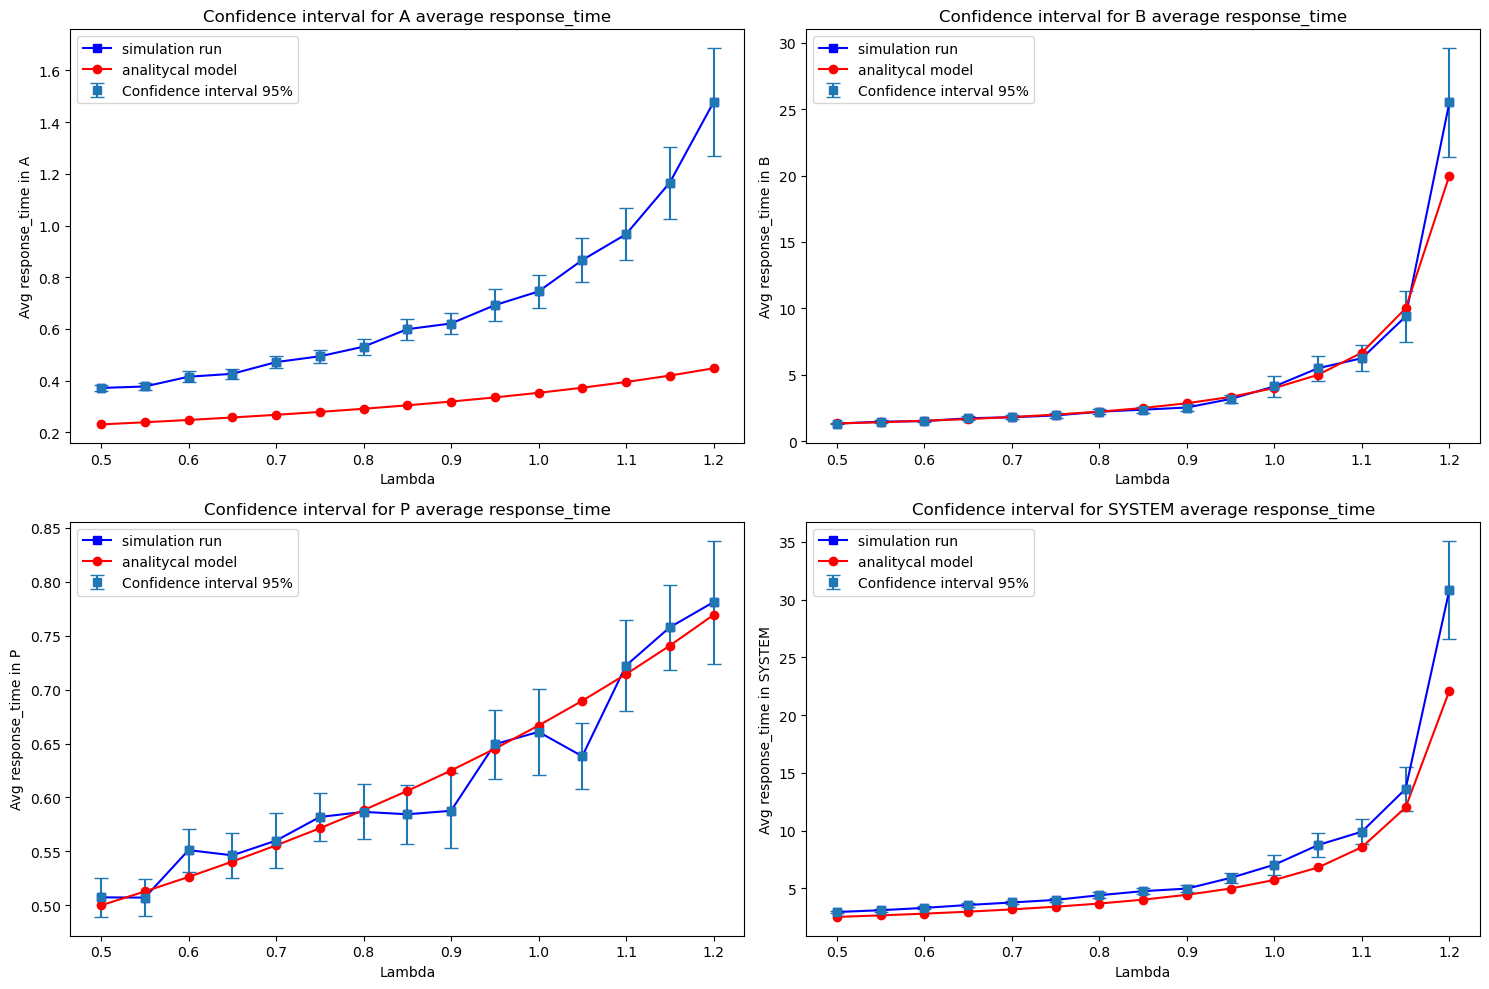
\includegraphics[width=\textwidth]{figs//results/obj1/obj1-line-response-time.png}
    \caption{Intervallo di confidenza del tempo di risposta medio e confronto con modello analitico per l'obiettivo 1}
    \label{fig:obj1_line_response_time}
\end{figure*}
\begin{figure*}
    \centering
    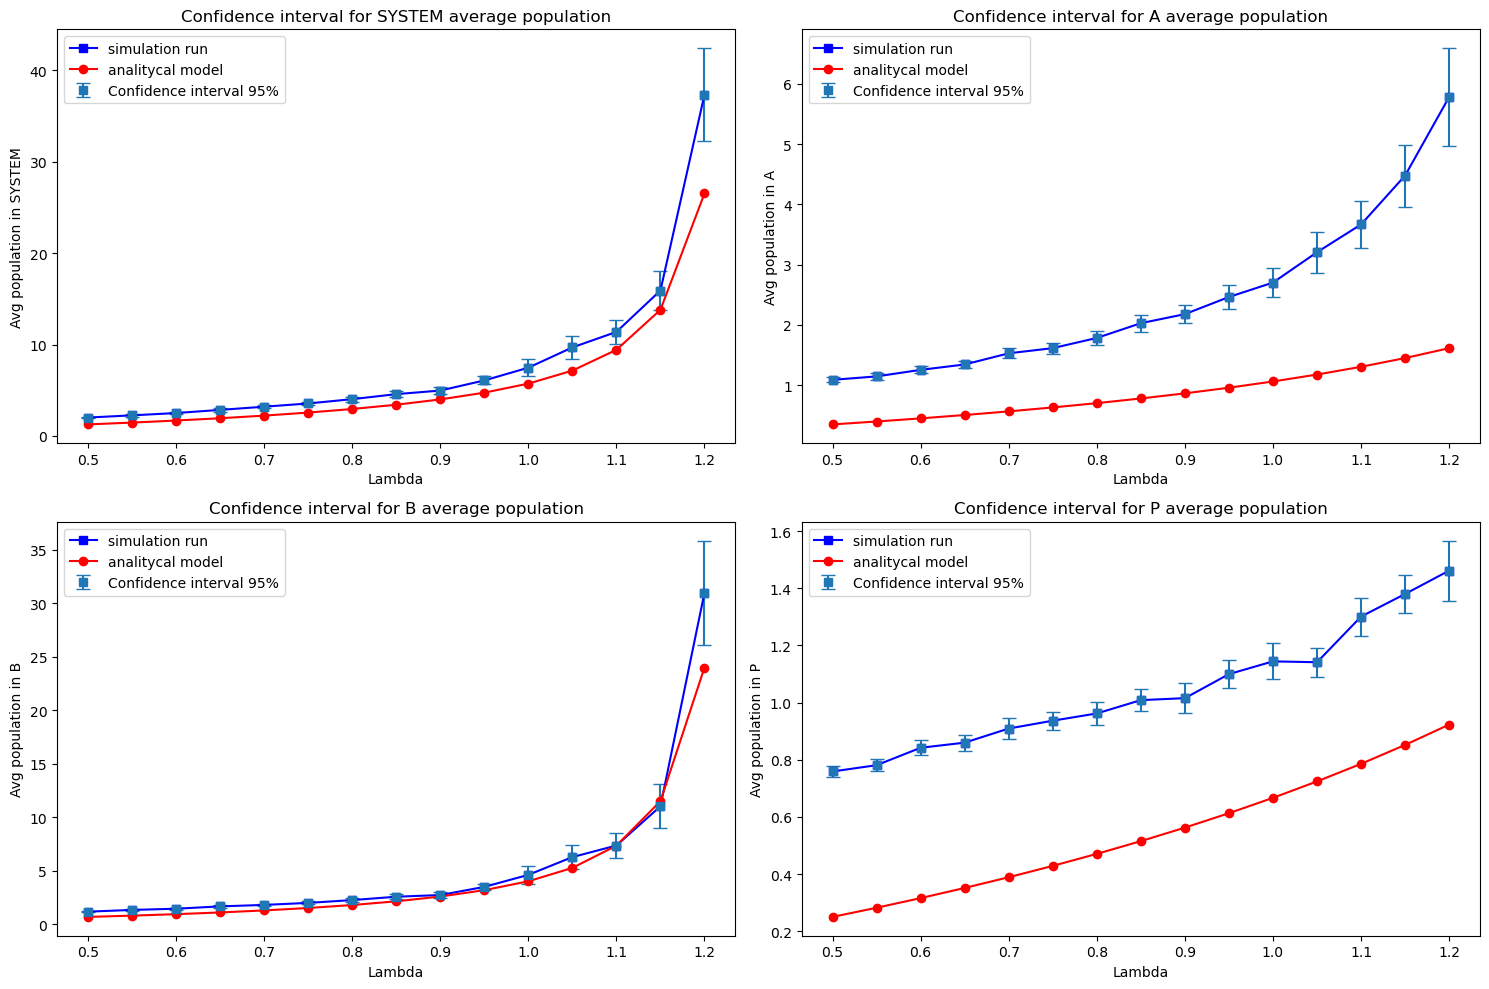
\includegraphics[width=\textwidth]{figs//results/obj1/obj1-line-population.png}
    \caption{Intervallo di confidenza della popolazione media e confronto con modello analitico per l'obiettivo 1}
    \label{fig:obj1_line_population}
\end{figure*}
\begin{figure*}
    \centering
    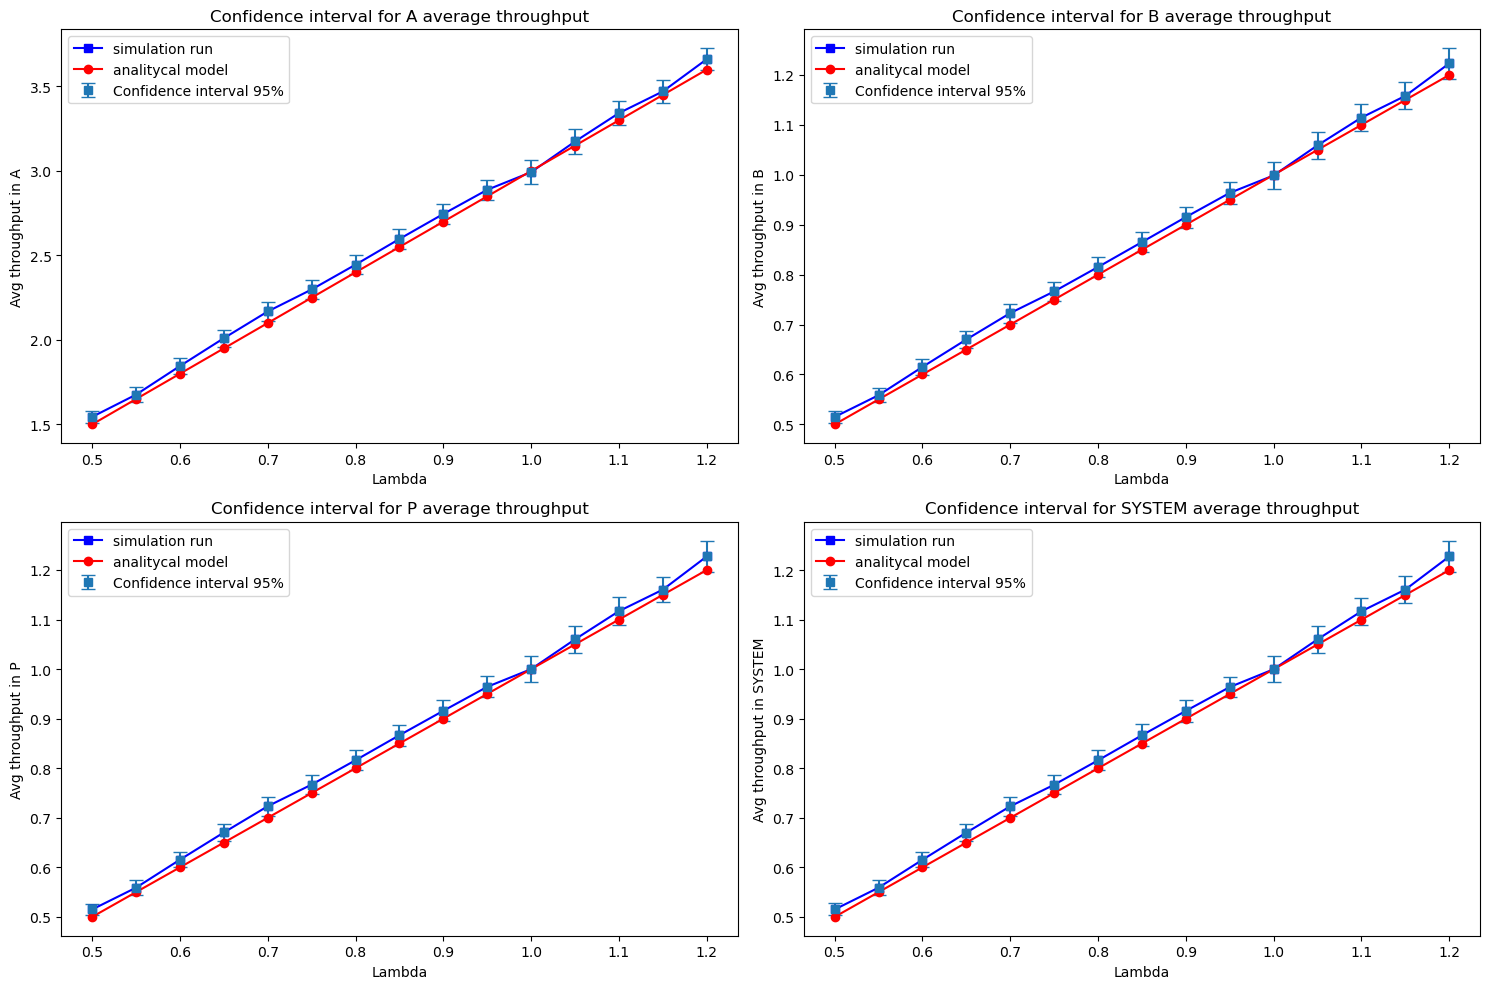
\includegraphics[width=\textwidth]{figs//results/obj1/obj1-line-throughput.png}
    \caption{Intervallo di confidenza del throughput medio e confronto con modello analitico per l'obiettivo 1}
    \label{fig:obj1_line_throughput}
\end{figure*}

Abbiamo effettuato in \autoref{fig:obj1_lineplots_utilization} i grafici anche per l'utilizzazione dei singoli nodi per effettuare i confronti con il modello analitico.\\
Come per il throughput anche in questo caso notiamo una forte aderenza tra i due modelli sempre con il server A più discostato rispetto agli altri due server.
\begin{figure*}
    \centering
    \begin{subfigure}{0.49\linewidth}
        \centering
        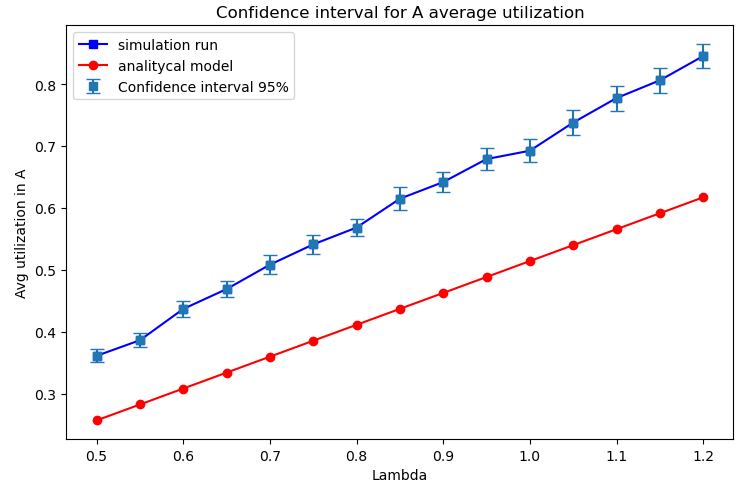
\includegraphics[width=\columnwidth]{figs/results/obj1/obj1-line-utilization-A.png}
        \caption{Server A}
        \label{fig:obj1_line_utilization_A}
    \end{subfigure} 
    \begin{subfigure}{0.49\linewidth}
        \centering
         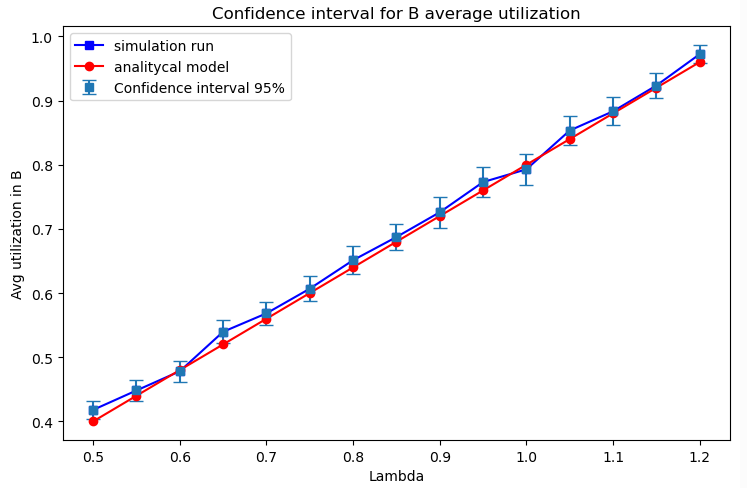
\includegraphics[width=\columnwidth]{figs/results/obj1/obj1-line-utilization-B.png}
        \caption{Server B}
        \label{fig:obj1_line_utilization_B}
    \end{subfigure}
    \begin{subfigure}{0.5\linewidth}
        \centering
        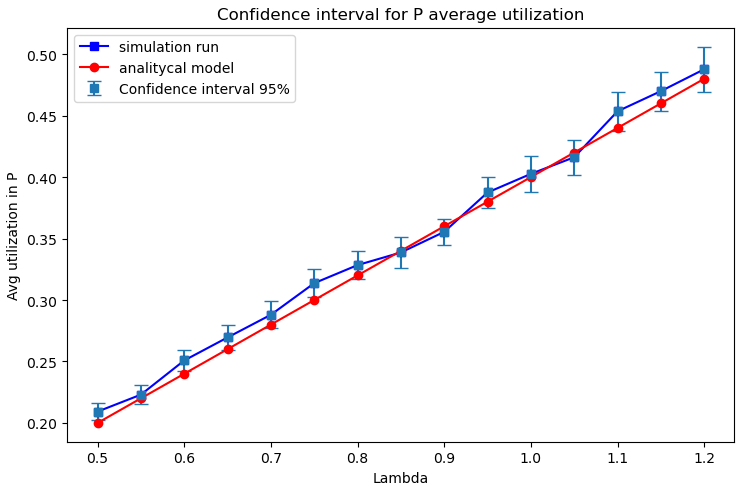
\includegraphics[width=\columnwidth]{figs/results/obj1/obj1-line-utilization-P.png}
        \caption{Server P}
        \label{fig:obj1_line_utilization_P}
    \end{subfigure}
    \caption{Intervallo di confidenza dell'utilizzazione e confronto con modello analitico per l'obiettivo 1.}
    \label{fig:obj1_lineplots_utilization}
\end{figure*}

\subsubsection{Validazione con il caso di studio}
Per la validazione dell'obiettivo 1 si faccia riferimento a \autoref{sec:results_obj2_validation}

\subsubsection{Analisi orizzonte finito}
\label{sec:results-obj1-transient}
Abbiamo infine eseguito una simulazione ad orizzonte finito con 100 run da 64 job ciascuna di cui si possono vedere i risultati in \autoref{fig:obj1_line_population-rep}, \autoref{fig:obj1_line_response_time-rep}, \autoref{fig:obj1_line_throughput-rep} sempre facendo il confronto con i dati ottenuti dal modello analitico, in questo caso notiamo come il modello differisce in maniera più evidente rispetto al caso dell'orizzonte finito, risultato atteso dato che sono statistiche ottenute dal sistema in stato transitorio.
\begin{figure*}
    \centering
    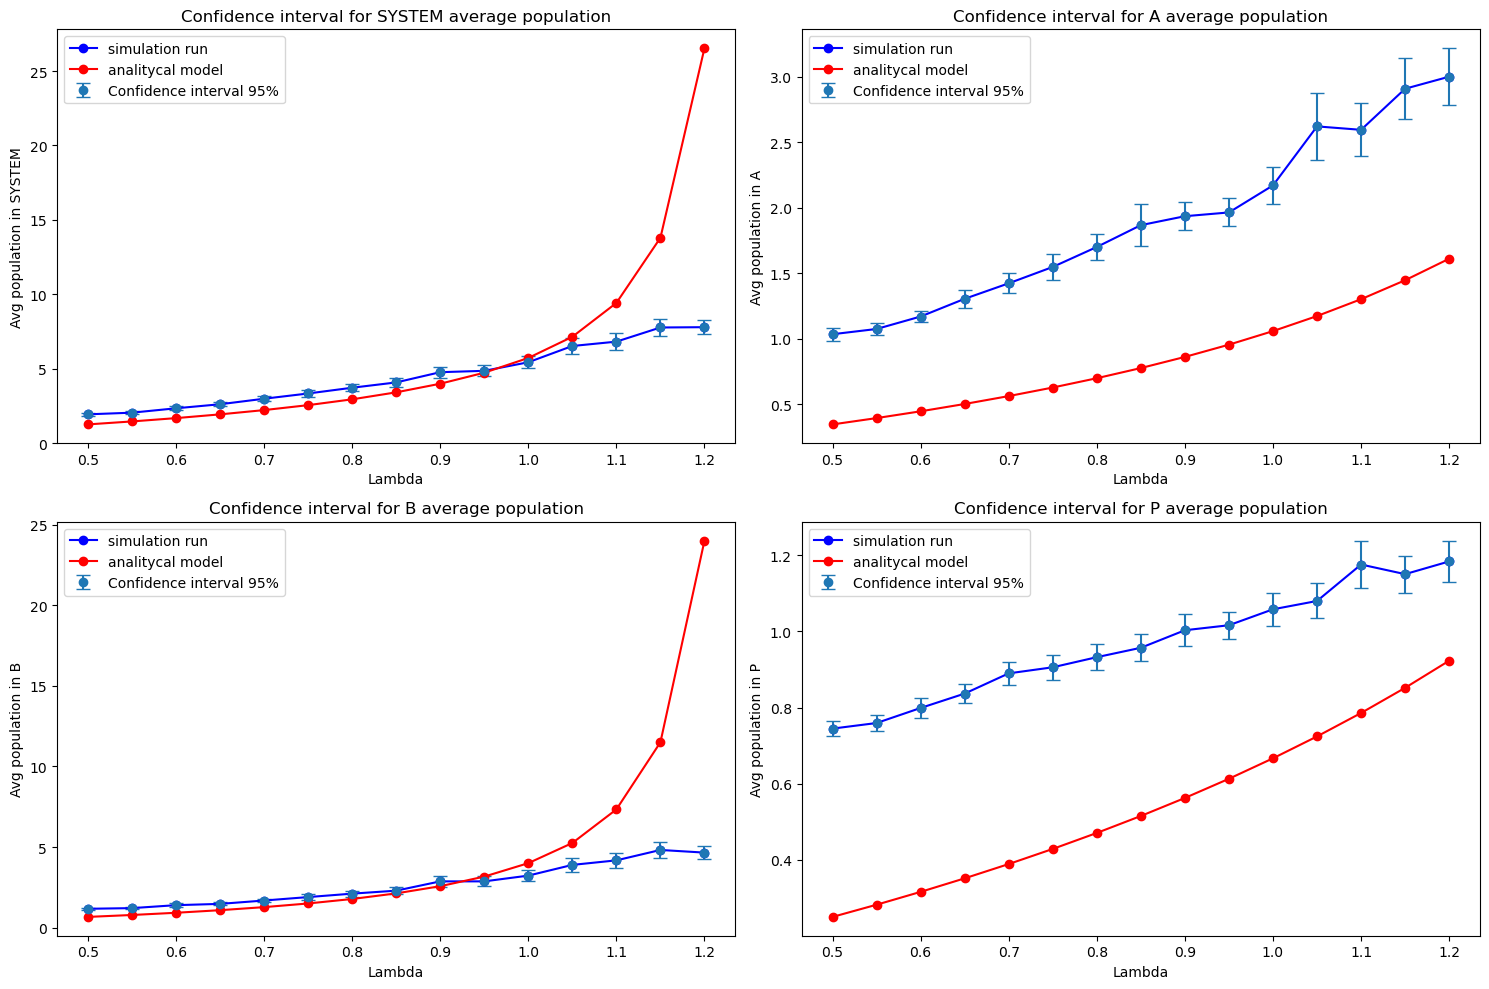
\includegraphics[width=\textwidth]{figs//results/obj1/obj1-line-population-rep.png}
    \caption{Intervallo di confidenza della popolazione media e confronto con modello analitico per l'obiettivo 1 ad orizzonte finito.}
    \label{fig:obj1_line_population-rep}
\end{figure*}
\begin{figure*}
    \centering
    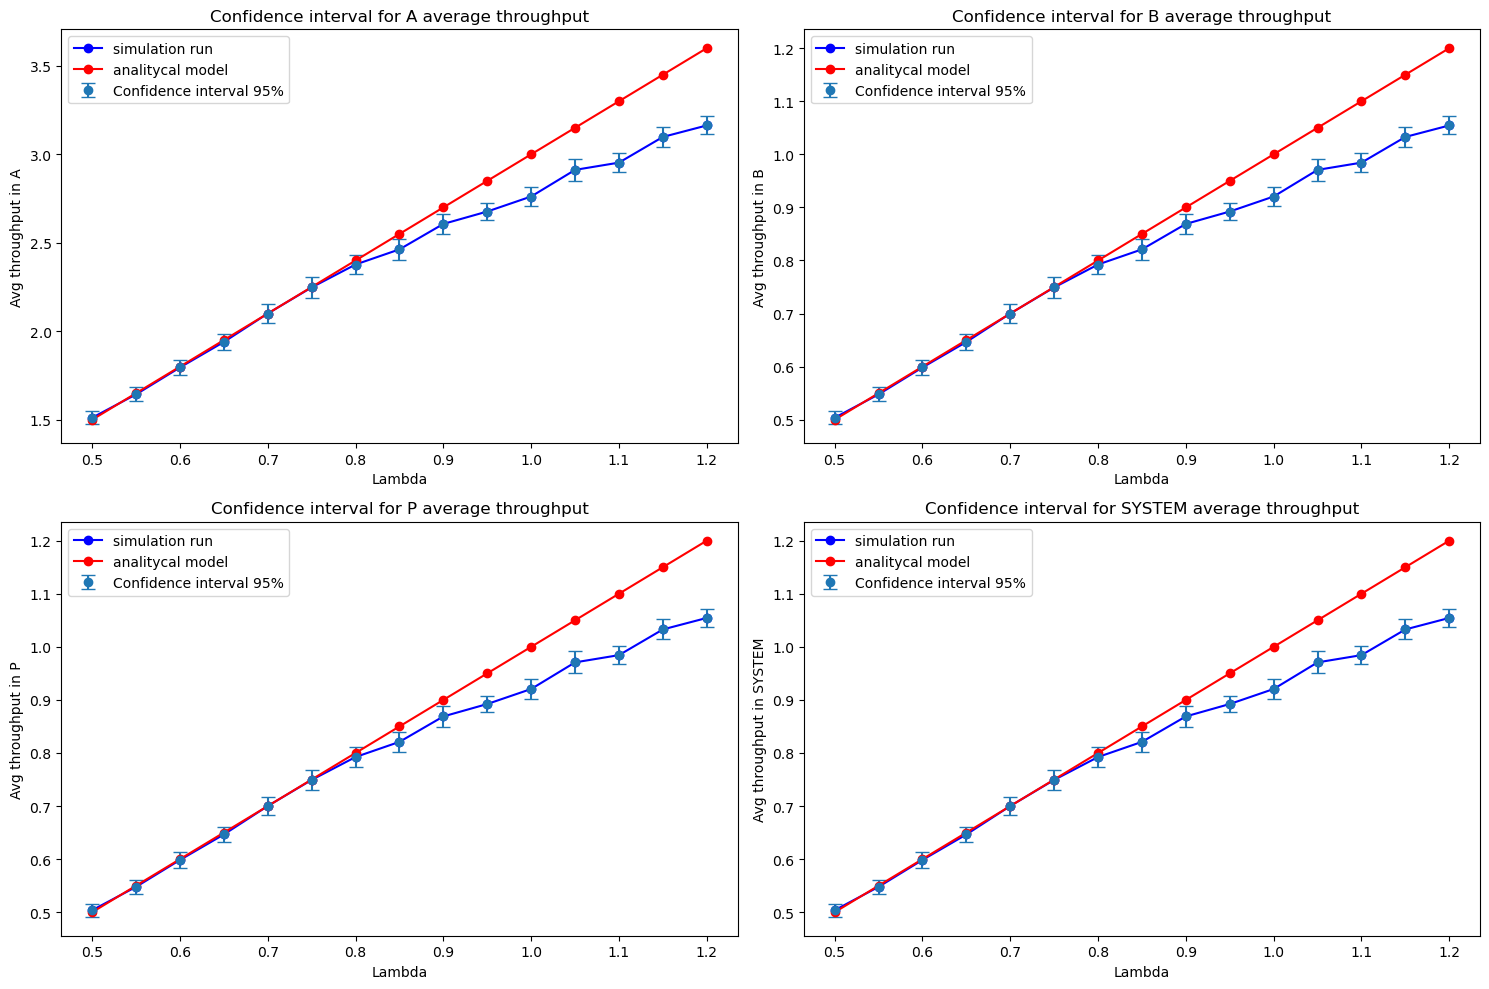
\includegraphics[width=\textwidth]{figs//results/obj1/obj1-line-throughput-rep.png}
    \caption{Intervallo di confidenza del throughput medio e confronto con modello analitico per l'obiettivo 1 ad orizzonte finito.}
    \label{fig:obj1_line_throughput-rep}
\end{figure*}
\begin{figure*}
    \centering
    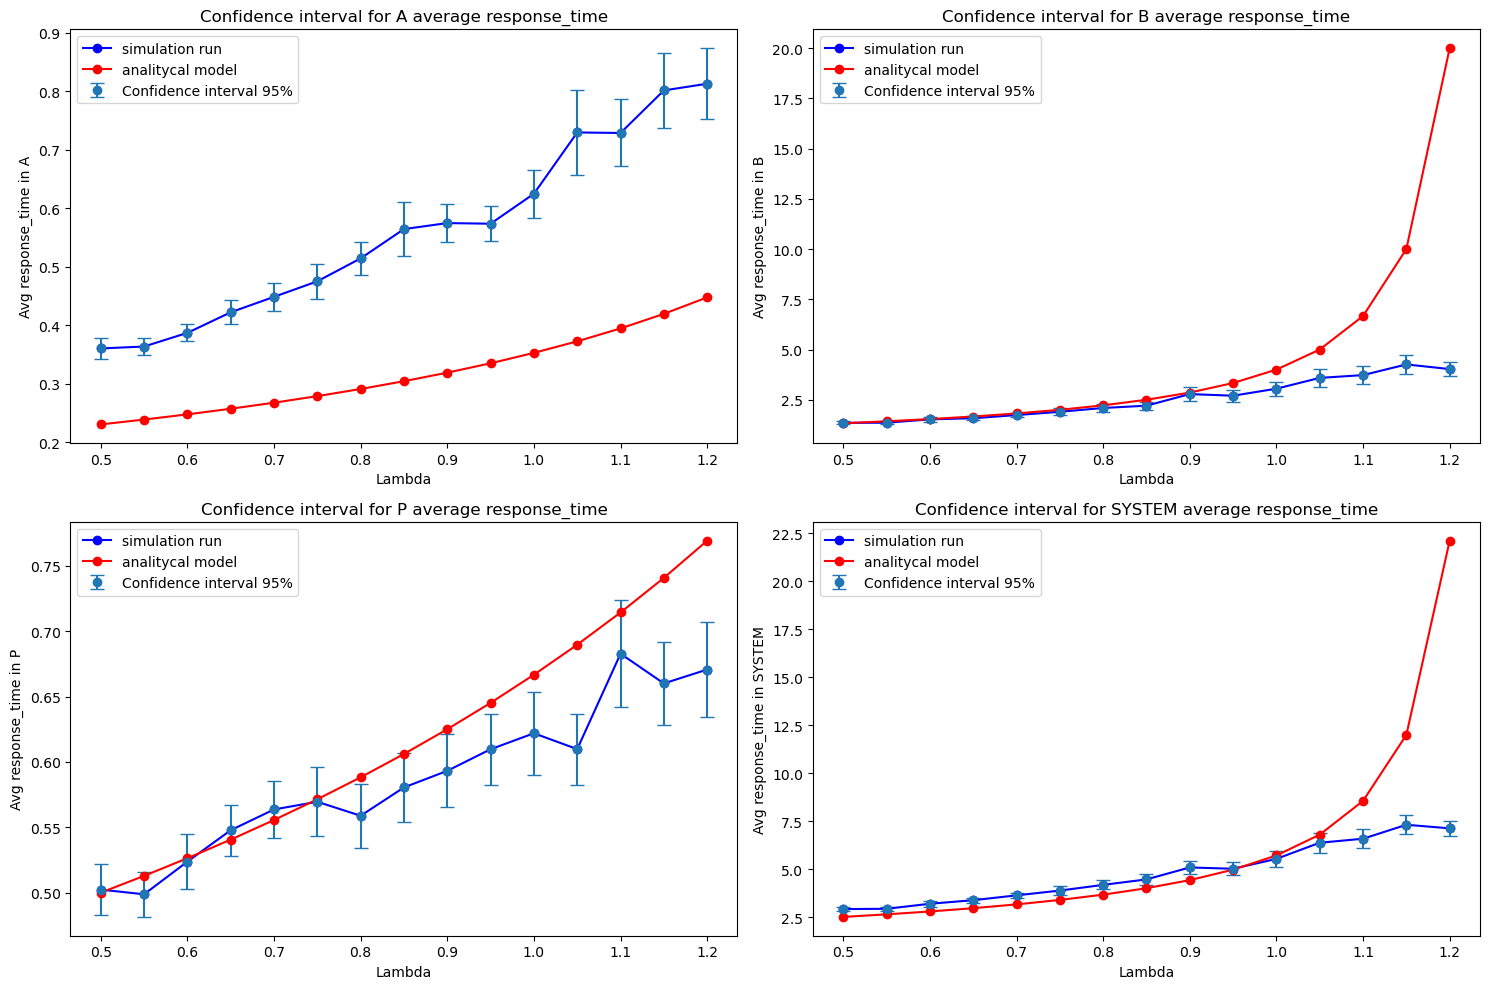
\includegraphics[width=\textwidth]{figs//results/obj1/obj1-line-response-time-rep.png}
    \caption{Intervallo di confidenza del tempo di risposta medio e confronto con modello analitico per l'obiettivo 1 ad orizzonte finito.}
    \label{fig:obj1_line_response_time-rep}
\end{figure*}


\subsection{Obiettivo 2}
\subsubsection{Infinite Horizon}
\begin{frame}{\subsecname: \subsubsecname}
    \begin{figure}
        \centering
        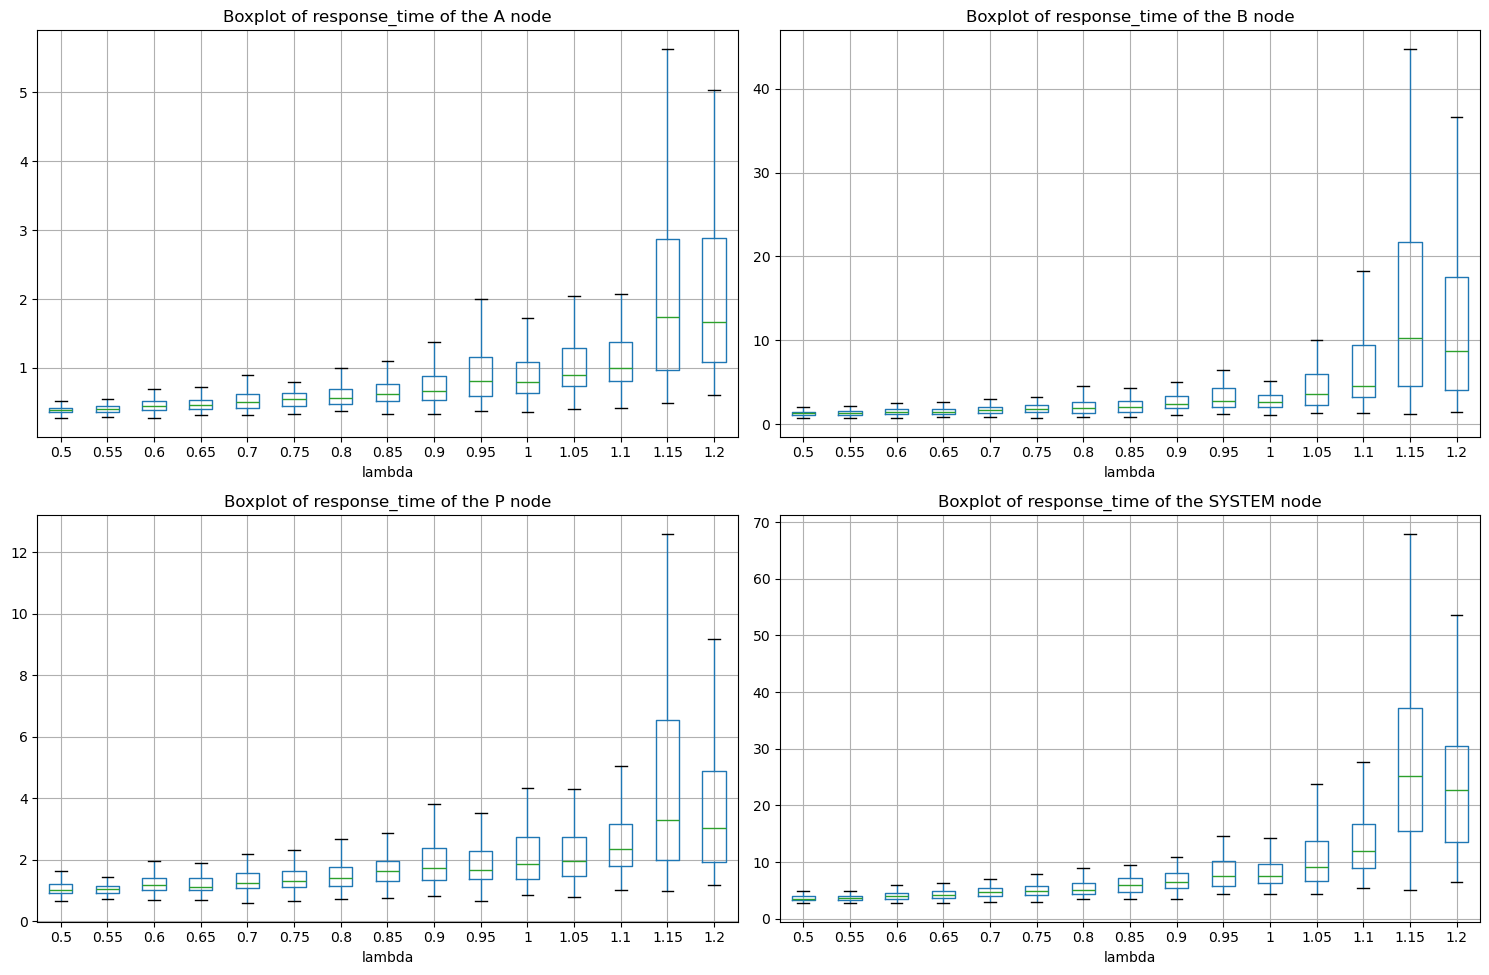
\includegraphics[width=0.75\linewidth]{figs/results/obj2/simulation/obj2_boxplot_rtime.png}
        \caption{Distribuzione del Tempo di Risposta medio dei risultati sperimentali dell’obbiettivo 2}
        \label{fig:enter-label}
    \end{figure}
\end{frame}

\subsubsection{Finite Horizon}
\begin{frame}{\subsecname: \subsubsecname}
    \begin{figure}
        \centering
        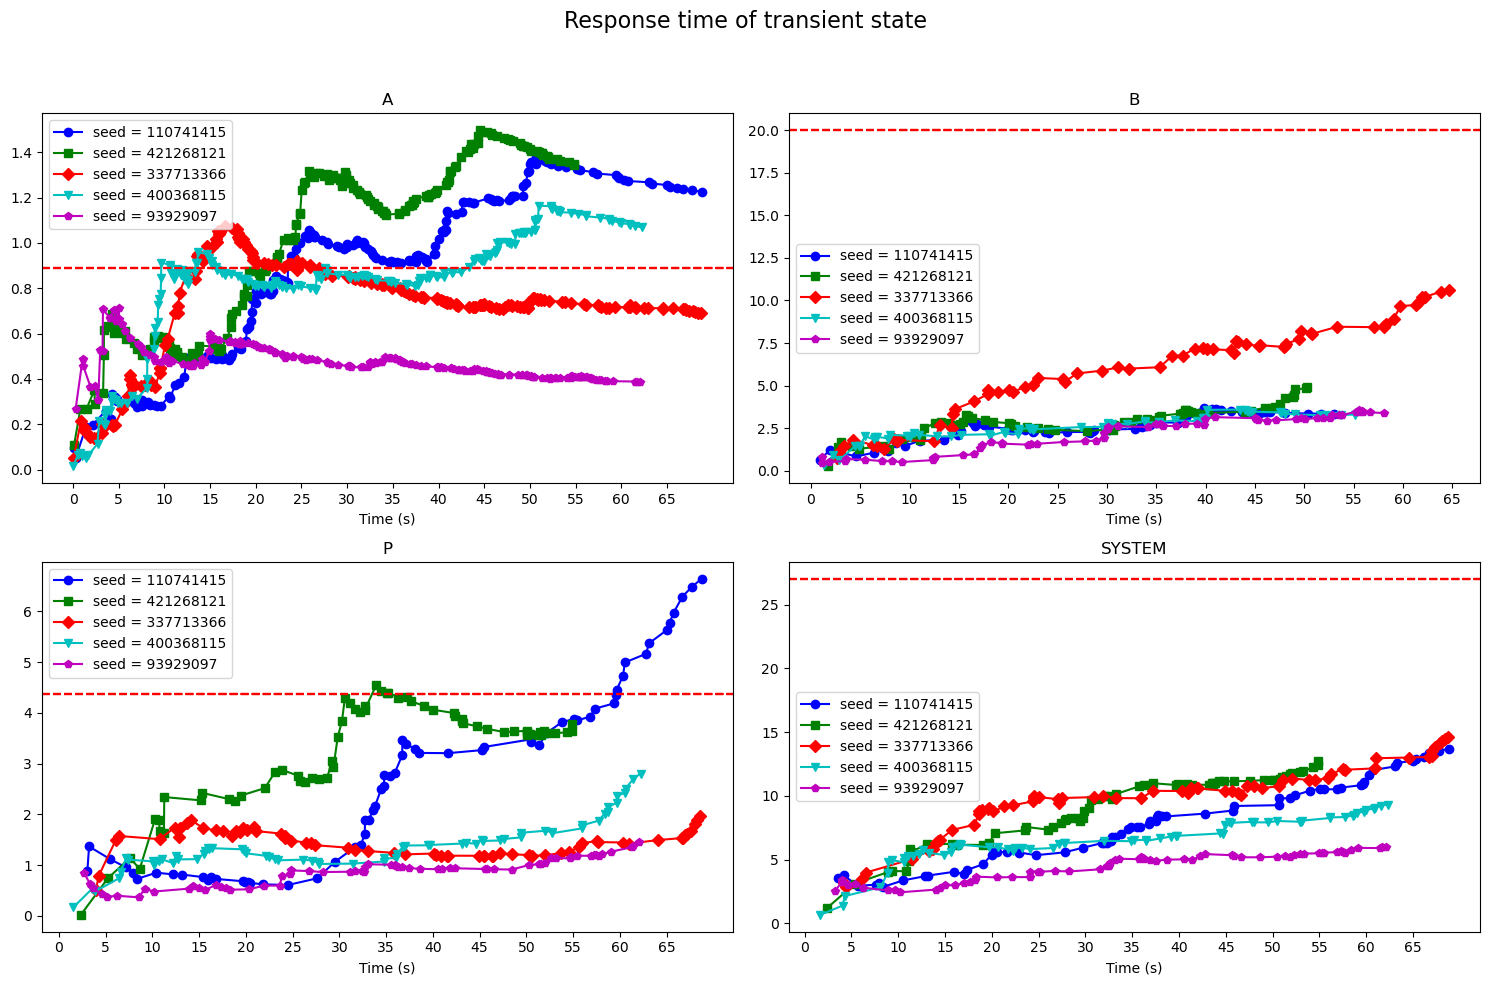
\includegraphics[width=0.75\linewidth]{figs/appendices/transient/obj2-transient-rtime-analitycal.png}
        \caption{Tempo di risposta per l’obiettivo 2 in funzione del tempo di simulazione nello stato transiente del sistema con un rate di arrivi 1.2 $job/s$ al variare del seed}
        \label{fig:enter-label}
    \end{figure}
\end{frame}

\subsubsection{Verification}
\begin{frame}{\subsecname: \subsubsecname}
\begin{figure}
    \centering
    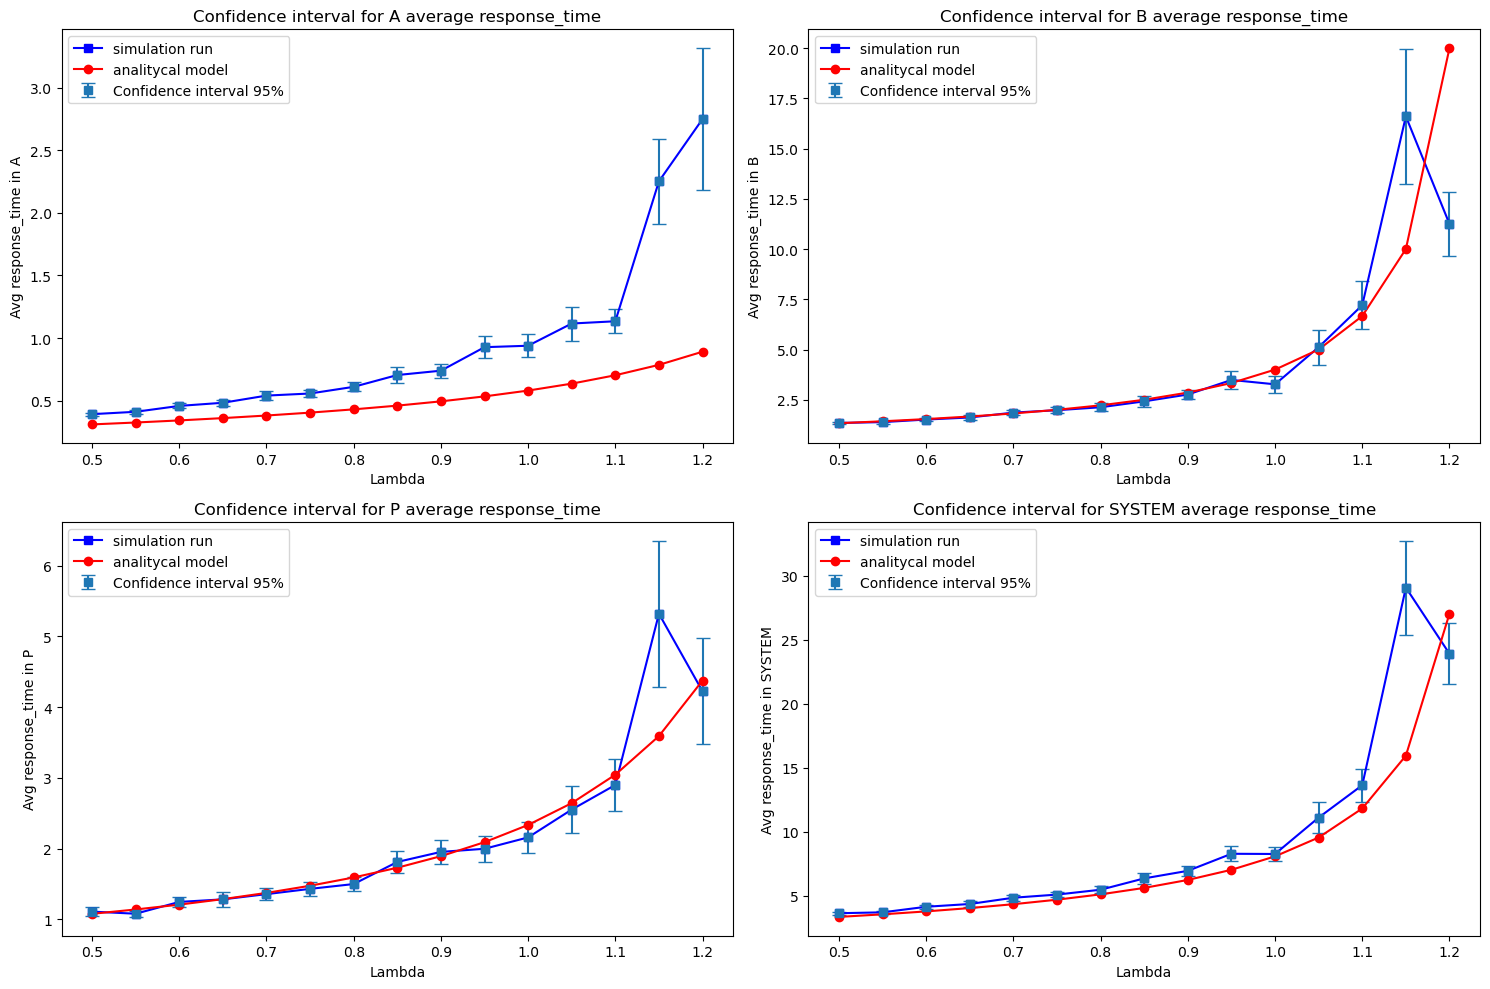
\includegraphics[width=0.75\linewidth]{figs/results/obj2/verification/obj2_lineplots_rtime.png}
    \caption{ Confronto tra valori medi della simulazione e del modello analitico del Tempo di Risposta per l’Obiettivo 2.}
    \label{fig:enter-label}
\end{figure}   
\end{frame}

\subsubsection{Validation}
\begin{frame}{\subsecname: \subsubsecname}
\begin{figure}
    \centering
    \begin{subfigure}{0.49\linewidth}
        \centering
        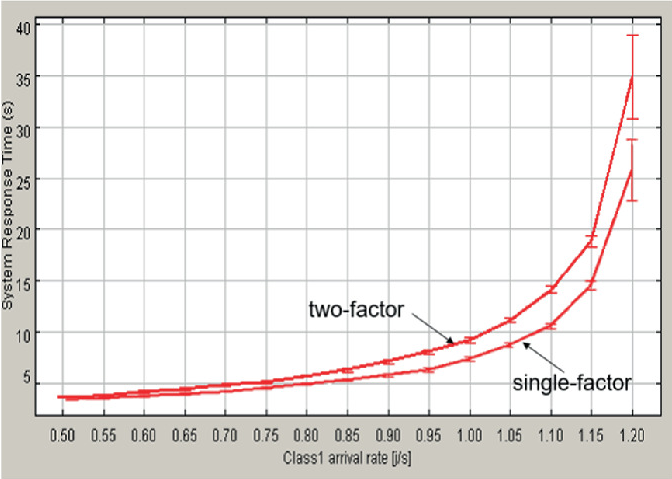
\includegraphics[width=1\linewidth]{figs/results/obj2/validation/casestudy_system_rtime.png}
        \caption{Case Study \citep{DBLP:books/sp/Serazzi24}}
        \label{fig:Single_VS_Two_FA_Perfomance_Comparison_population}
    \end{subfigure}
    % \hfill
    \begin{subfigure}{0.49\linewidth}
        \centering
        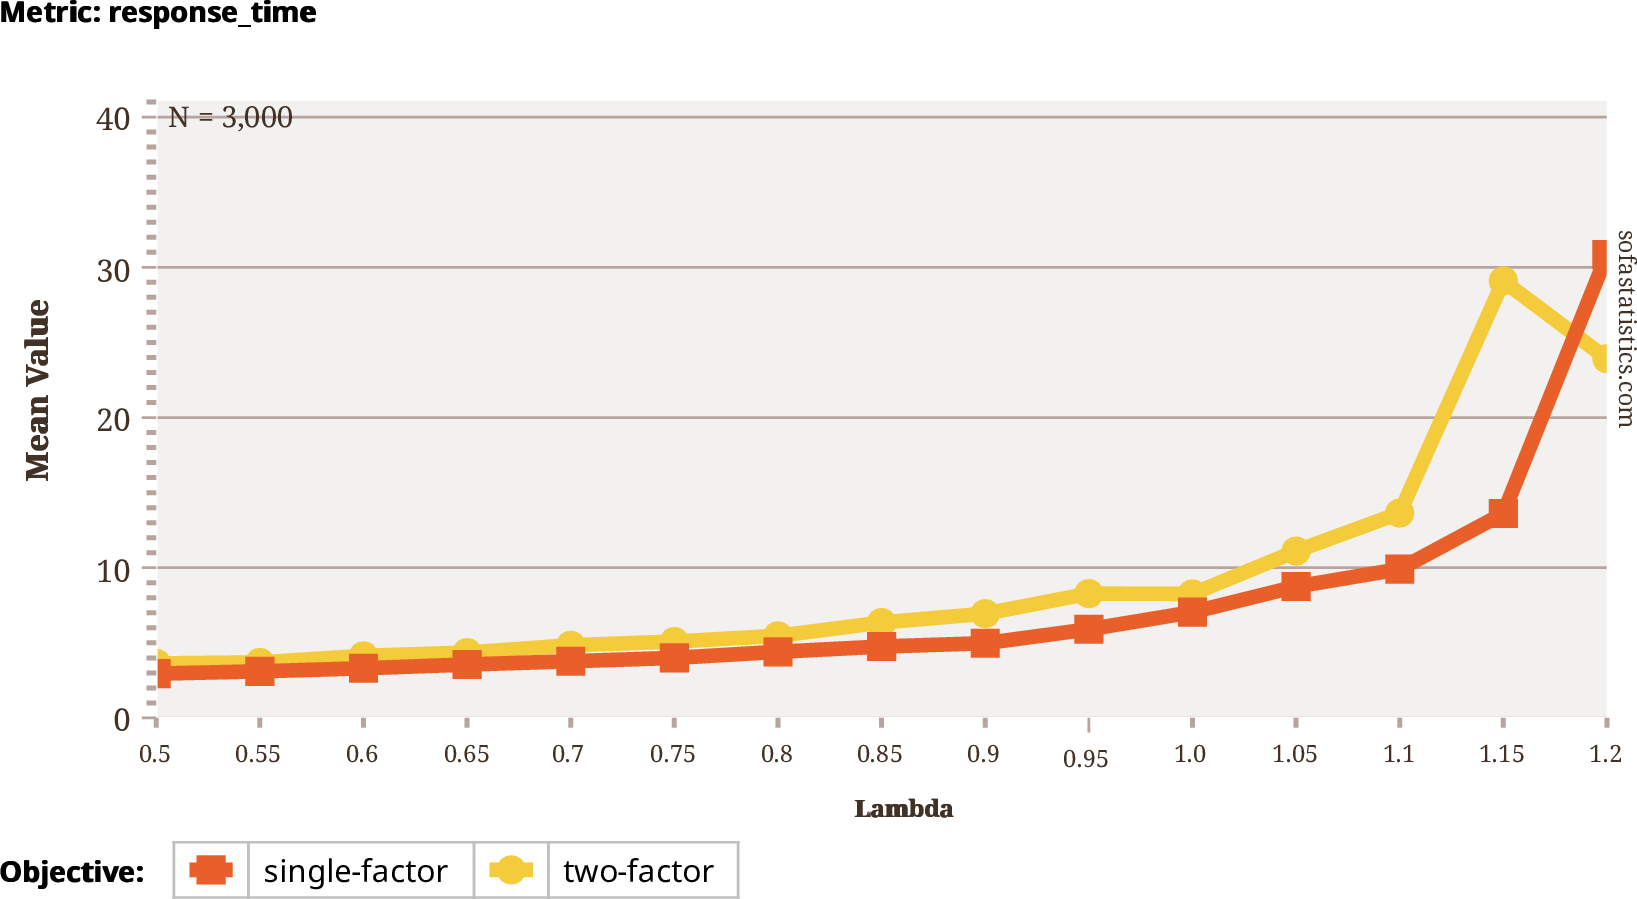
\includegraphics[width=1\linewidth]{figs/results/obj2/validation/single_VS_Two_FA_Perfomance_Comparison_rtime.png}
        \caption{Simulazione}
        \label{fig:Single_VS_Two_FA_Perfomance_Comparison_rtime}
    \end{subfigure}
    % \hfill
    \caption{Tempo di Risposta medi del sistema in funzione del rate di arrivi esterni nel caso con e senza 2FA.}
    \label{fig:Single_VS_Two_FA_Perfomance_Comparison}
\end{figure}
\end{frame}


\subsection{Obiettivo 3}
\subsubsection{Infinite Horizon}
\begin{frame}{\subsecname: \subsubsecname}
    \begin{figure}
        \centering
        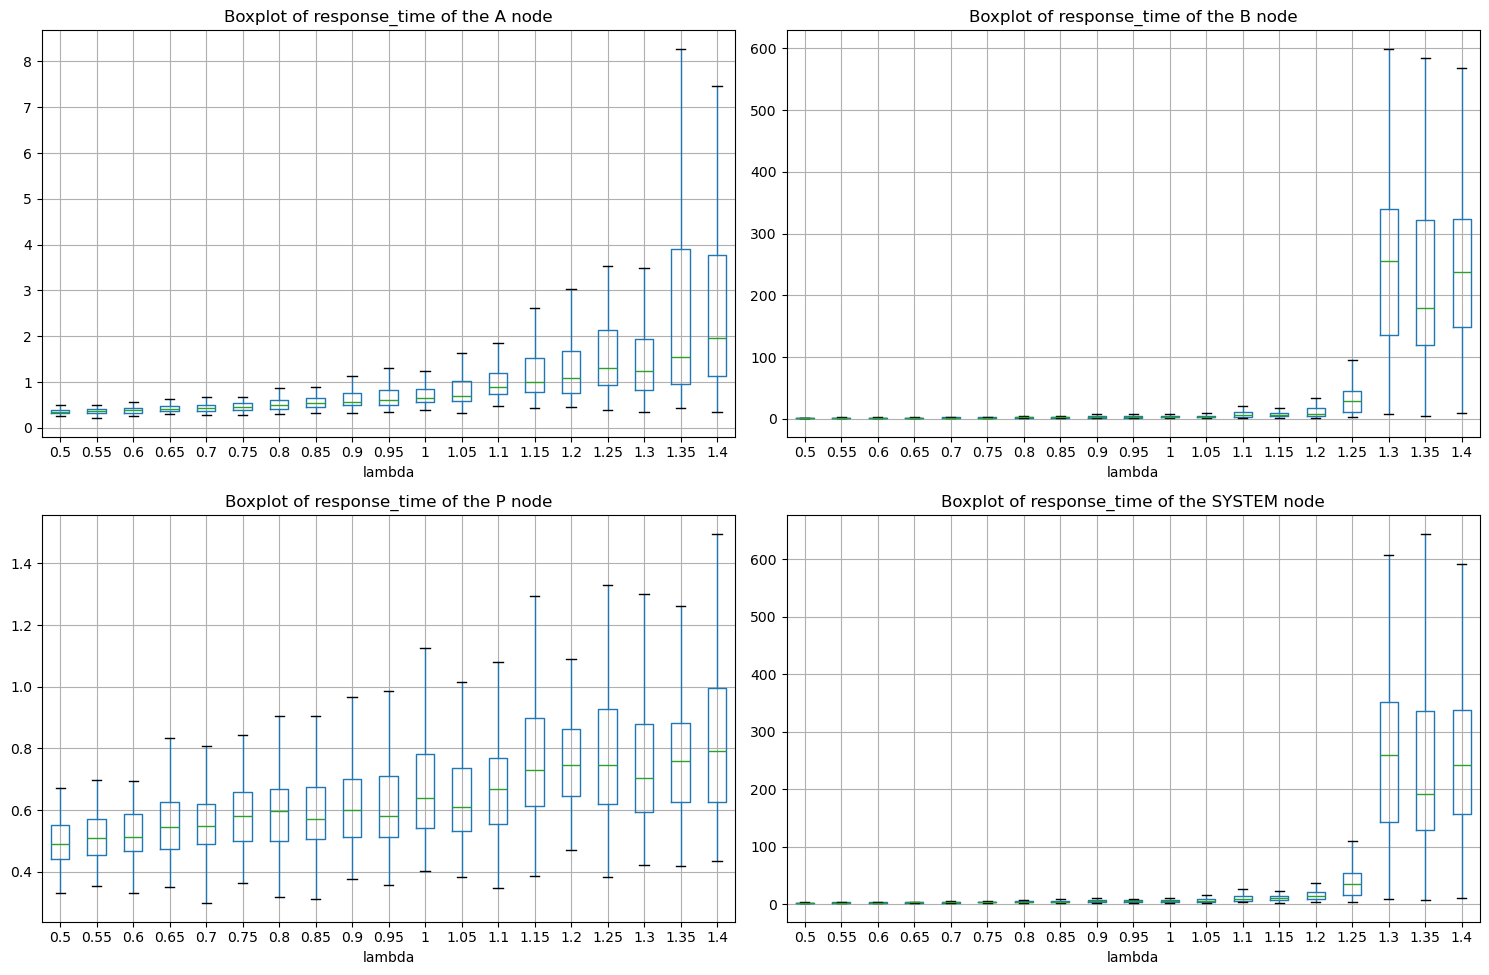
\includegraphics[width=0.75\linewidth]{figs/results/obj3/simulation/obj3_boxplot_rtime.png}
        \caption{Distribuzione del Tempo di Risposta medio dei risultati sperimentali dell’obbiettivo 3}
        \label{fig:enter-label}
    \end{figure}
\end{frame}

\subsubsection{Finite Horizon}
\begin{frame}{\subsecname: \subsubsecname}
    \begin{figure}
        \centering
        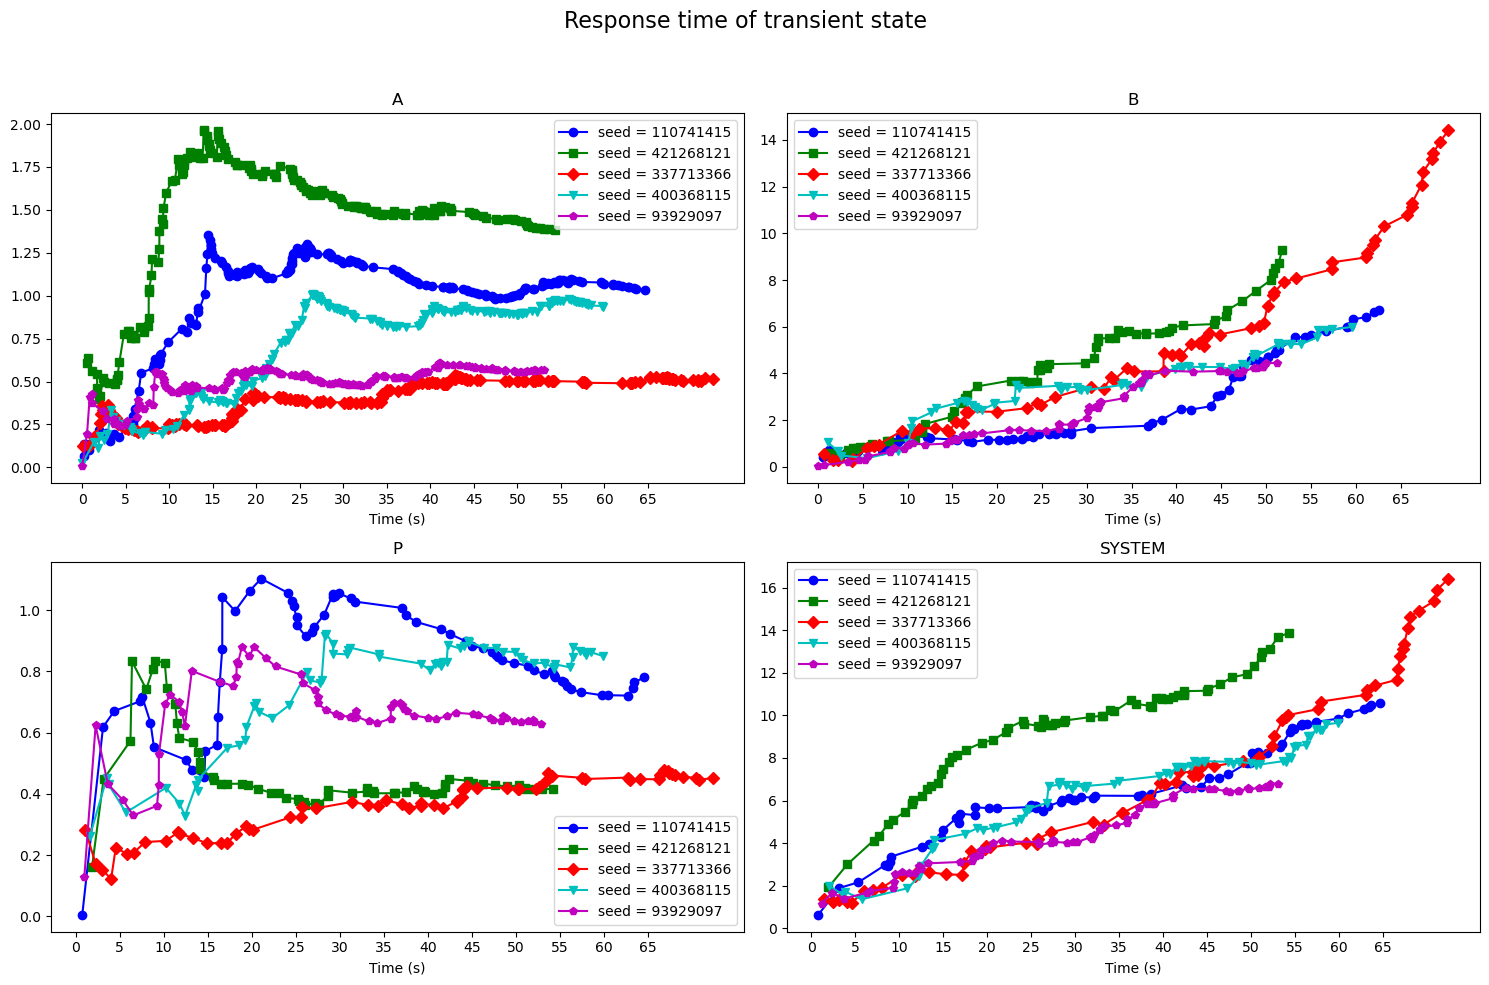
\includegraphics[width=0.75\linewidth]{figs/appendices/transient/obj3-transient-rtime-analitycal.png}
        \caption{Tempo di risposta per l’obiettivo 3 in funzione del tempo di simulazione nello stato transiente del sistema con un rate di arrivi 1.4 $job/s$ al variare del seed}
        \label{fig:enter-label}
    \end{figure}
\end{frame}

\subsubsection{Verification}
\begin{frame}{\subsecname: \subsubsecname}
\begin{figure}
    \centering
    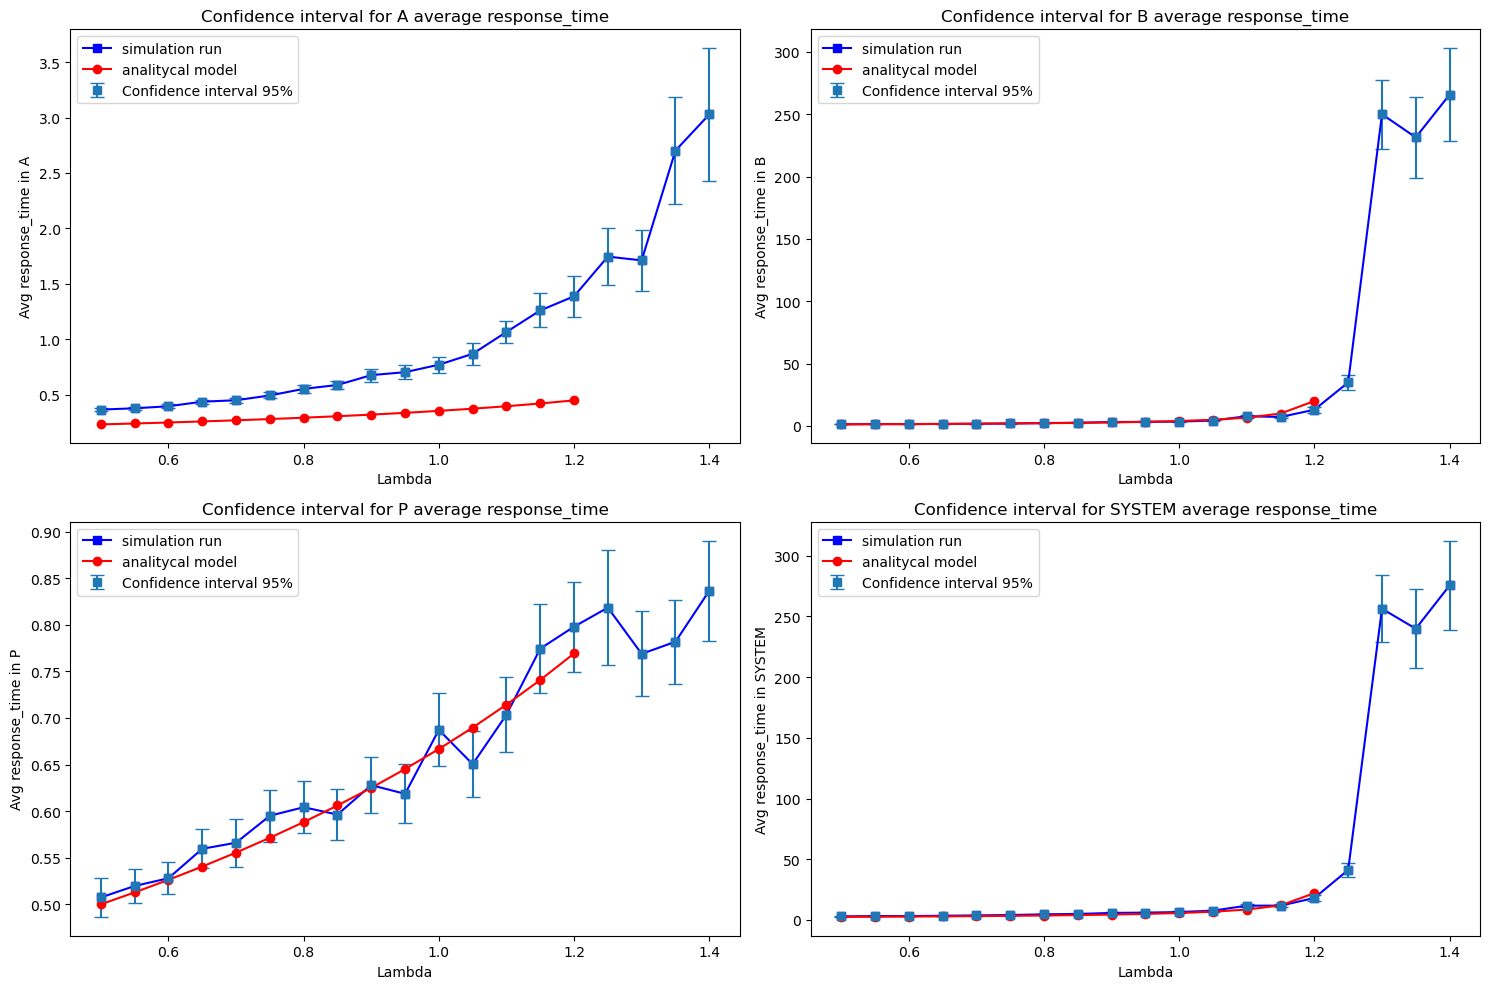
\includegraphics[width=0.75\linewidth]{figs/results/obj3/verification/obj3_lineplot_rtime.png}
    \caption{ Confronto tra valori medi della simulazione e del modello analitico dell Tempo di Risposta per l’Obiettivo 3.}
    \label{fig:enter-label}
\end{figure}   
\end{frame}

\subsection{Obiettivo 4}
\subsubsection{Throughput comparison}
\begin{frame}{\subsecname: \subsubsecname}
    \begin{figure}
        \centering
        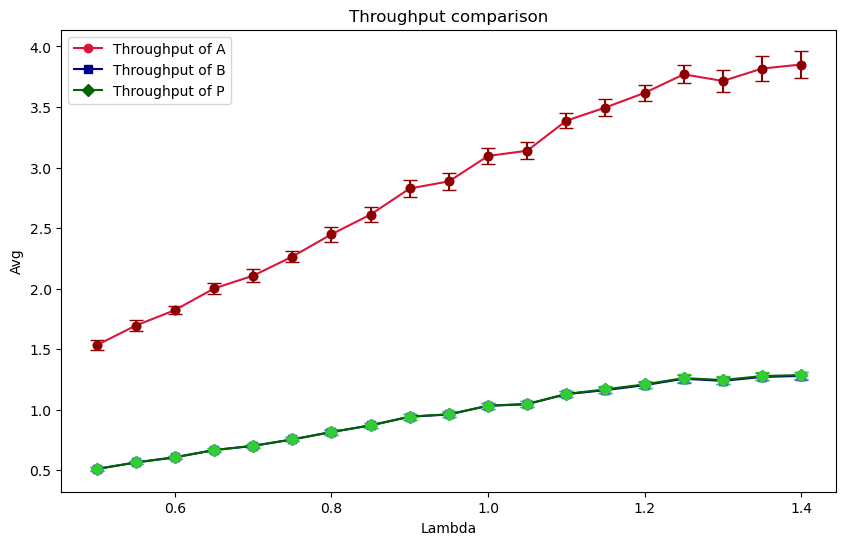
\includegraphics[width=0.75\linewidth]{figs/results/obj4/obj4-throughput-comparison.png}
        \caption{Confronto tra throughput dei tre server con tasso di arrivo $1.4 job/s$}
        \label{fig:enter-label}
    \end{figure}
\end{frame}

\subsubsection{Service time from 0.8 to 0.4}
\begin{frame}{\subsecname: \subsubsecname}
    \begin{figure}
        \centering
        \begin{subfigure}{0.49\linewidth}
            \centering
            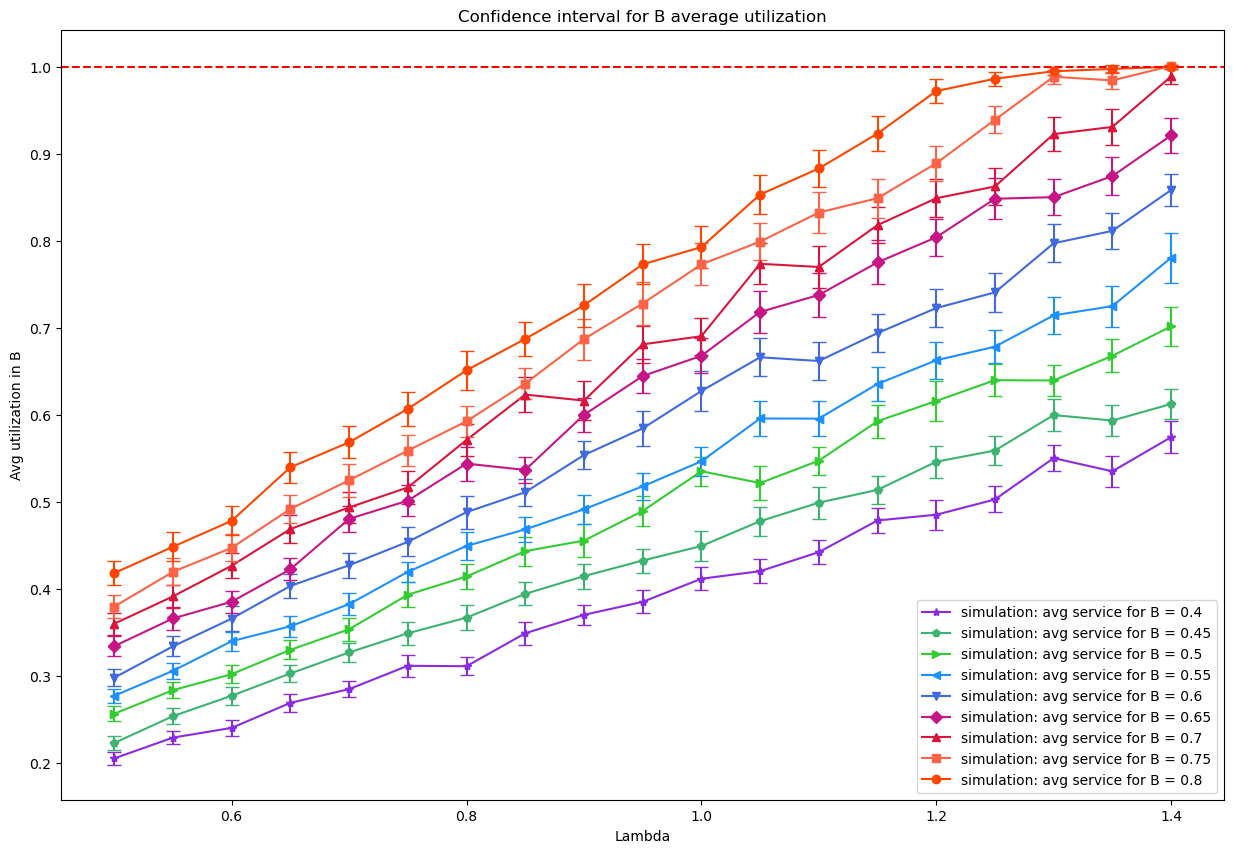
\includegraphics[width=\linewidth]{figs/results/obj4/obj4-utilization-service-time.png}
            \caption{Utilizzazione}
            \label{fig:obj4_utilization_service-time}
        \end{subfigure}
        \hfill
        \begin{subfigure}{0.49\linewidth}
            \centering
            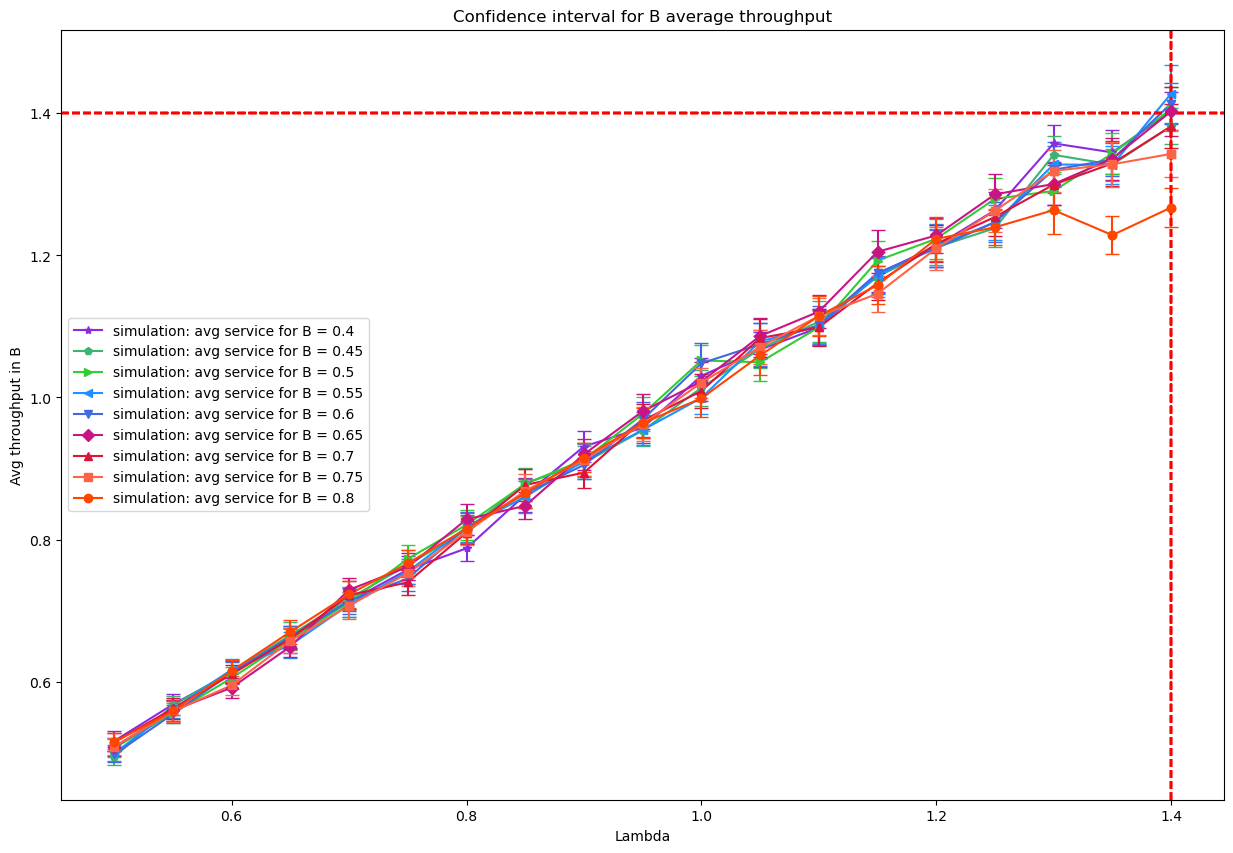
\includegraphics[width=\linewidth]{figs/results/obj4/obj4-throughput-service-time.png}
            \caption{Throughput}
            \label{fig:obj4_throughput_service-time}
        \end{subfigure}
        \caption{Confronto Throughput e Utilizzazione medi al variare dei valori dei tempi di servizio}
        \label{fig:obj4-service-time-comparison}
    \end{figure}
\end{frame}

\subsubsection{Service time 0.4 vs 0.65}
\begin{frame}{\subsecname: \subsubsecname}
    \begin{table}
        \centering
        \begin{tabularx}{\textwidth}{X X}
            \begin{minipage}{0.48\textwidth}
                \centering
                \caption{Minimi e massimi di utilizzazione e throughput per tempi di servizio 0.65 del server B}
                \begin{tabular}{ccc}
                    $\lambda$ & metrica & valore\\
                    0.5 & utilizzazione & 0.333898\\
                    1.4 & utilizzazione & 0.921304\\
                    0.5 & throughput & 0.507752\\
                    1.4 & throughput & 1.40273
                \end{tabular}
                \label{tab:065_metrics}
            \end{minipage}
            &
            \begin{minipage}{0.48\textwidth}
                \centering
                \caption{Minimi e massimi di utilizzazione e throughput per tempi di servizio 0.4 del server B}
                \begin{tabular}{ccc}
                    $\lambda$ & metrica & valore\\
                    0.5 & utilizzazione & 0.20484\\
                    1.4 & utilizzazione & 0.574275\\
                    0.5 & throughput & 0.516347\\
                    1.4 & throughput & 1.40302
                \end{tabular}
                \label{tab:04_metrics}
            \end{minipage}
        \end{tabularx}
    \end{table}
\end{frame}

\subsubsection{Finite Horizion (service time 0.4)}
\begin{frame}{\subsecname: \subsubsecname}
    \begin{figure}
        \centering
        \begin{subfigure}{\linewidth}
            \centering
            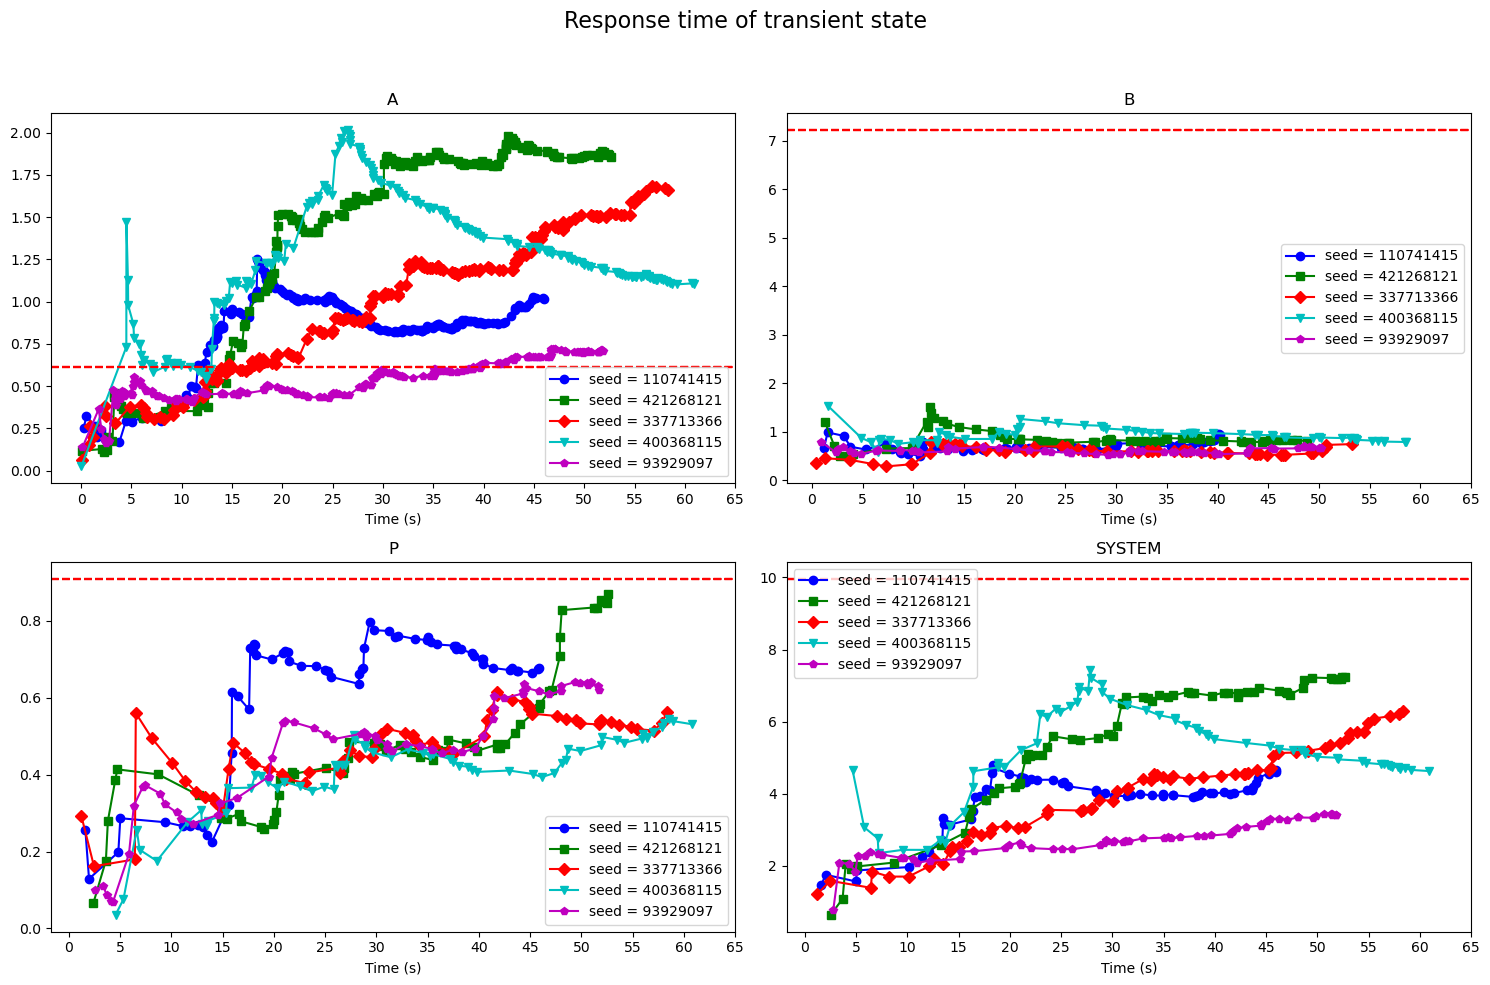
\includegraphics[width=0.8\linewidth]{figs/appendices/transient/obj4_04-transient-rtime-analitycal.png}
            \caption{Senza valore analitico}
            \label{fig:obj4_04_transient_simulation}
            \end{subfigure} 
        \begin{subfigure}{\linewidth}
            \centering
            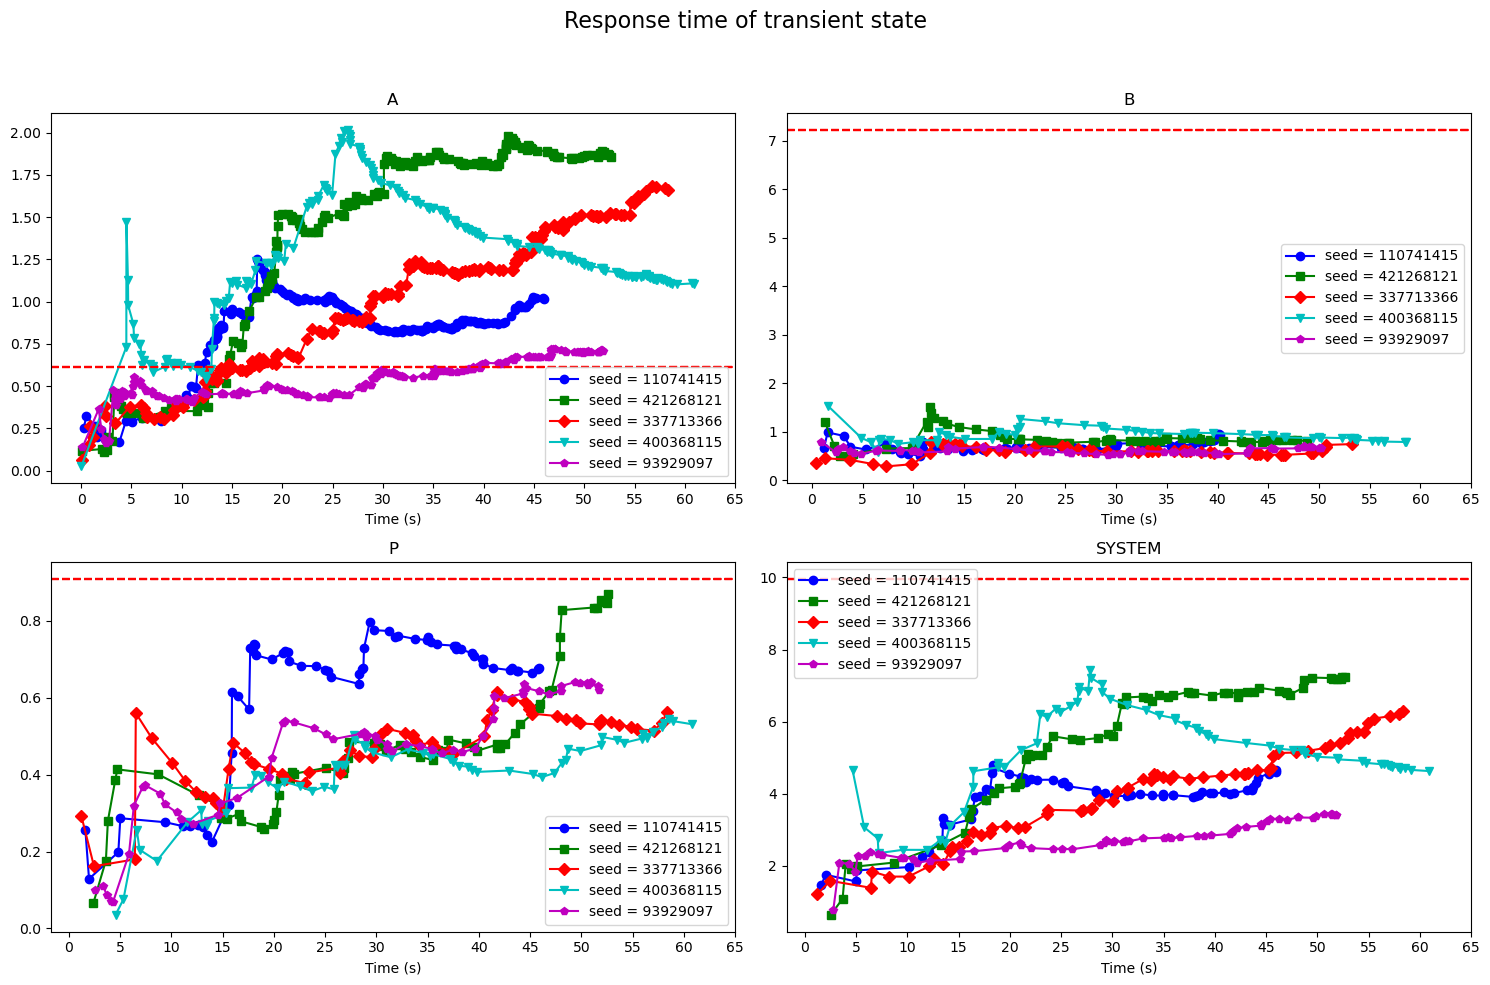
\includegraphics[width=0.8\linewidth]{figs/appendices/transient/obj4_04-transient-rtime-analitycal.png}
            \caption{Con valore analitico}
            \label{fig:obj4_04_transient_analitycal}
            \end{subfigure}
        \caption{Tempo di risposta per l'obiettivo 4 (con il server B con tempi di servizio 0.4s) in funzione del tempo di simulazione nello stato transiente del sistema con un rate di arrivi 1.4$job/s$ al variare del seed.}
        \label{fig:obj4_04_transient}
    \end{figure}
\end{frame}


\subsubsection{Verification (service time 0.4)}
\begin{frame}{\subsecname: \subsubsecname}
    \begin{figure}
        \centering
        \begin{subfigure}{0.35\linewidth}
            \centering
            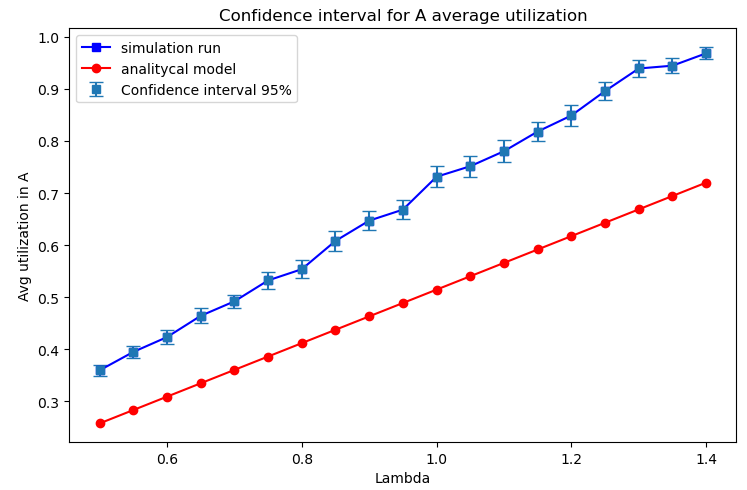
\includegraphics[width=\linewidth]{figs/results/obj4/obj4-utilizzazione-A.png}
            \label{fig:obj4_line_utilization_A}
        \end{subfigure} 
        \begin{subfigure}{0.35\linewidth}
            \centering
             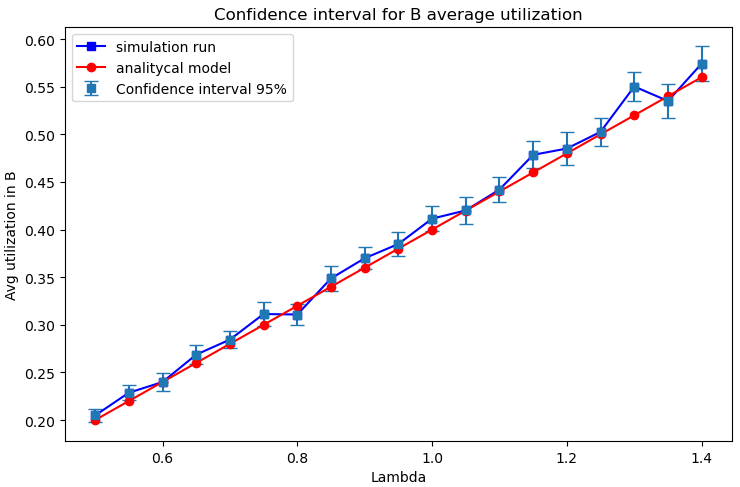
\includegraphics[width=\linewidth]{figs/results/obj4/obj4-utilizzazione-B.png}
            \label{fig:obj4_line_utilization_B}
        \end{subfigure}
        \begin{subfigure}{0.35\linewidth}
            \centering
            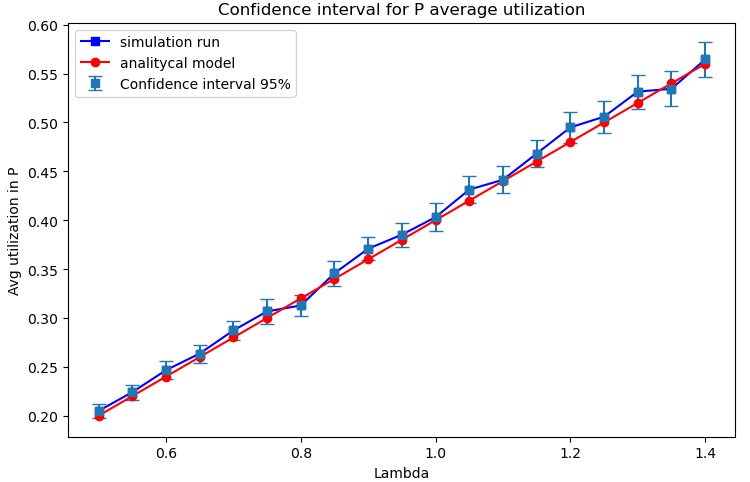
\includegraphics[width=\linewidth]{figs/results/obj4/obj4-utilizzazione-P.png}
            \label{fig:obj4_line_utilization_P}
        \end{subfigure}
        \caption{Intervallo di confidenza dell'utilizzazione e confronto con modello analitico per l'obiettivo 4.}
        \label{fig:obj4_lineplots_utilization}
    \end{figure}   
\end{frame}

\subsubsection{Validation}
\begin{frame}{\subsecname: \subsubsecname}
    \begin{figure}
        \centering
        \begin{subfigure}[b]{0.49\textwidth}
            \centering
            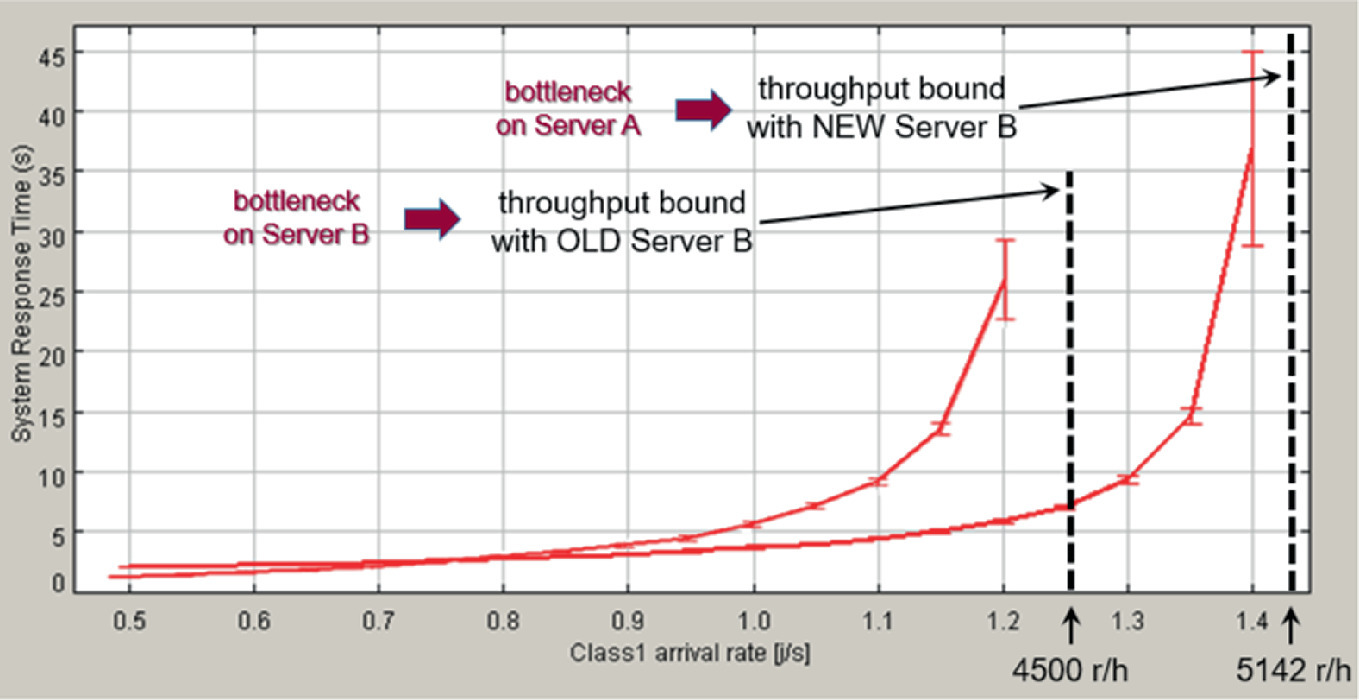
\includegraphics[width=\columnwidth]{figs/results/obj4/obj4-validazione.jpg}
            \caption{Caso di studio \citep{DBLP:books/sp/Serazzi24}}
            \label{fig:obj4_validazione_casestudy}
        \end{subfigure}
        \begin{subfigure}[b]{0.49\textwidth}
            \centering
            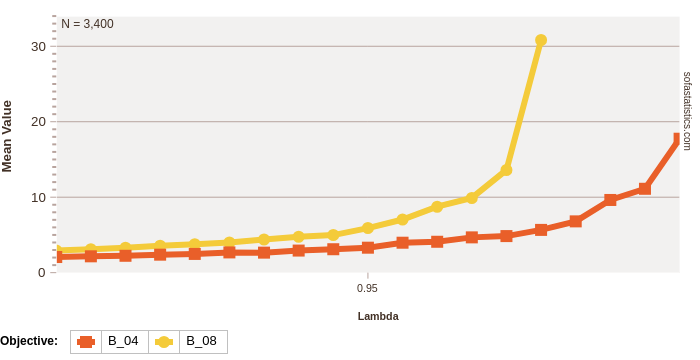
\includegraphics[width=\columnwidth]{figs/results/obj4/obj4-simulazione-validazione.png}
            \caption{Risultati sperimentali}
            \label{fig:obj4_validazione_simulation}
        \end{subfigure}
        \hfill
        \caption{Tempo di risposta medio prima e dopo la miglioria del server B in funzione del rate medio degli arrivi esterni}
        \label{fig:obj4_validazione}
    \end{figure}
\end{frame}


\bibliographystyle{ACM-Reference-Format}
\bibliography{paper/bibliography}

\appendix

\section{Appendice: Studio dello Stato Transitorio}
In questa appendice sono riportati i risultati per lo studio dello stato transitorio, divisi per obiettivi. Per ogni obiettivo, dato un set di 5 seed diversi, è stata simulata una replica per ogni seed con il rate di arrivi più alto previsto per poter studiarne il comportamento nel contesto di stress maggiore. Ricordiamo che i valori tabellari dei risultati esposti in questa sezione sono disponibili a \url{https://github.com/caballo-domestico/webapp-workflow-pa/blob/main/docs/plots/model_plots.ipynb}.

\subsection{Obiettivo 1}

In \autoref{fig:obj1_transient} è riportato il valore del Tempo di Risposta medio al variare del tempo di simulazione e del seed iniziale, con un rate di arrivi medio di $1.2 job/s$. Il valore, nonostante cresca notevolmente entro i primi momenti della simulazione, sembra assestarsi verso un valore compreso tra $1.3$ e $0.5s$ per il Server A. Inoltre, sembra che il server A riceva la maggior parte degli arrivi entro i primi 25 secondi di simulazione, per poi smaltire le richieste accumulate. Il Tempo di risposta per il sistema sembra crescere continuamente, per quattro dei cinque seed di simulazione. I server A e P sembrano avvicinarsi ai corrispettivi valori teorici, mentre B trascina l'intero sistema lontano da essi.

\begin{figure*}
    \centering
    \begin{subfigure}{\linewidth}
        \centering
        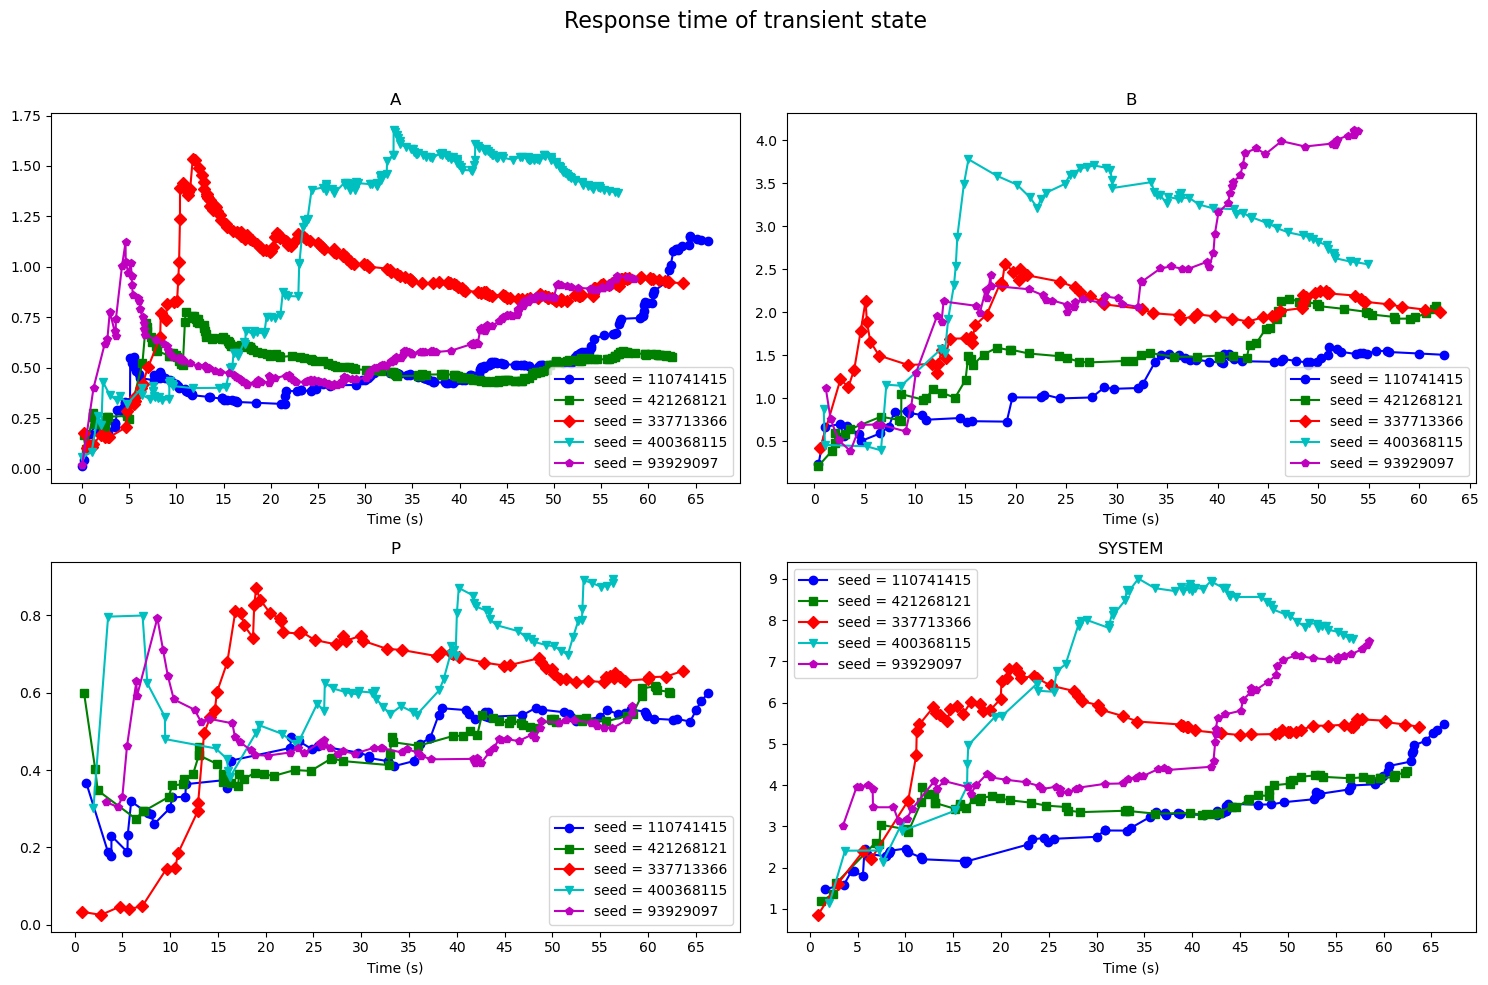
\includegraphics[width=0.8\linewidth]{figs/appendices/transient/obj1-transient-rtime.png}
        \caption{Senza valore analitico}
        \label{fig:obj1_transient_simulation}
        \end{subfigure} 
    \begin{subfigure}{\linewidth}
        \centering
        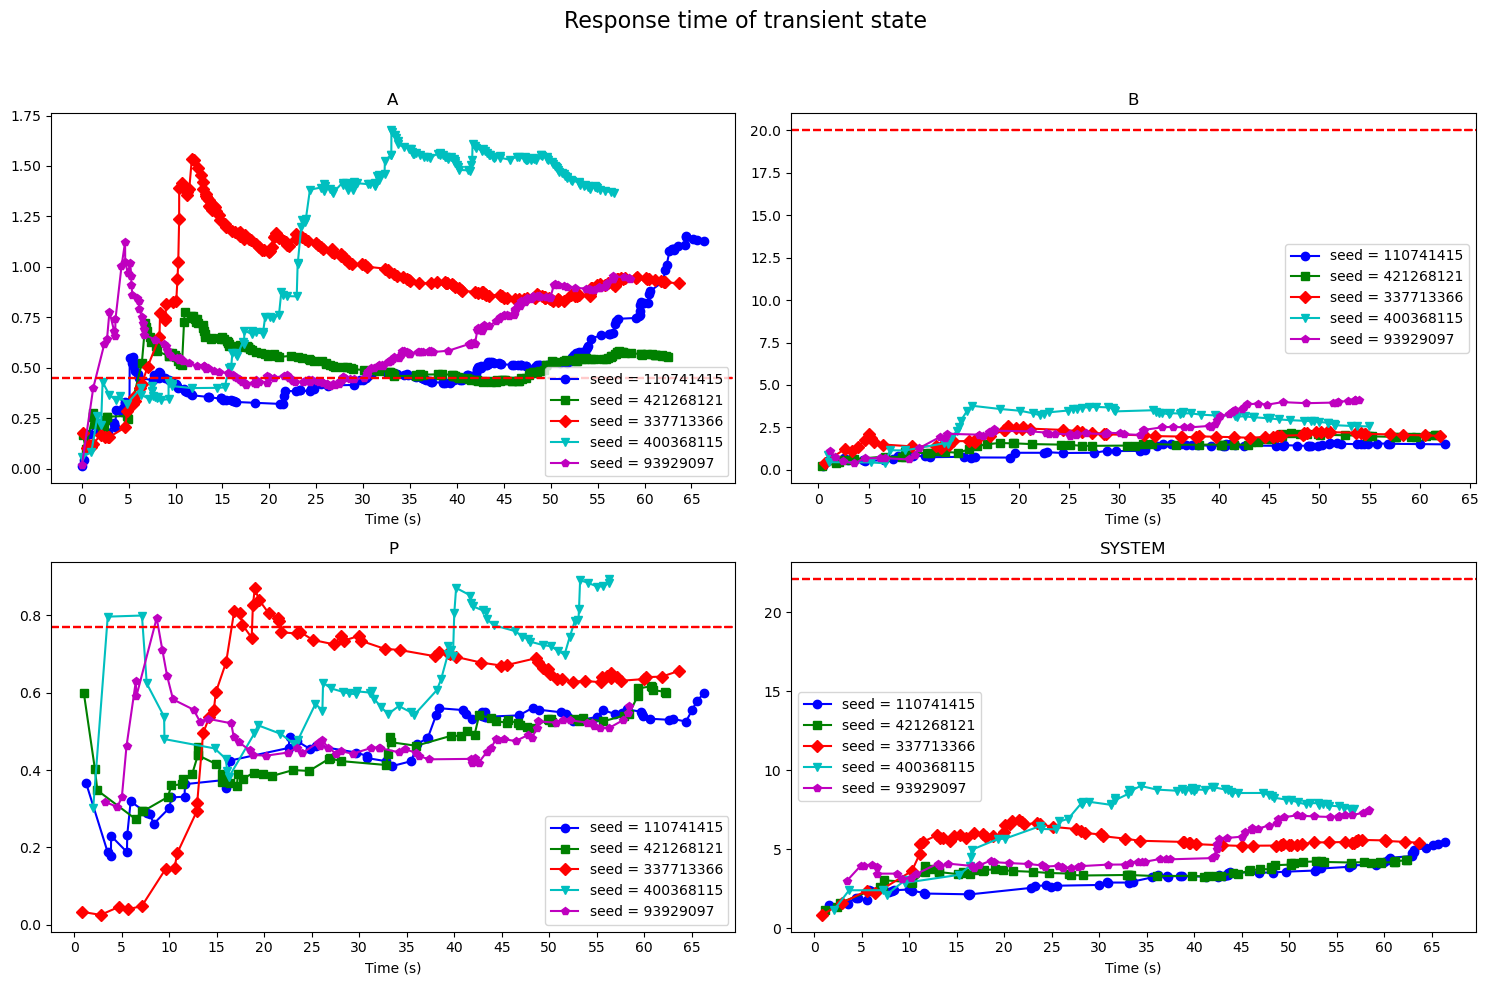
\includegraphics[width=0.8\linewidth]{figs/appendices/transient/obj1-transient-rtime-analitycal.png}
        \caption{Con valore analitico}
        \label{fig:obj1_transient_analitycal}
        \end{subfigure}
    \caption{Tempo di risposta per l'obiettivo 1 in funzione del tempo di simulazione nello stato transiente del sistema con un rate di arrivi 1.2$job/s$ al variare del seed.}
    \label{fig:obj1_transient}
\end{figure*}


\subsection{Obiettivo 2}

In \autoref{fig:obj2_transient} è riportato il valore del Tempo di Risposta medio al variare del tempo di simulazione e del seed iniziale, con un rate di arrivi medio di $1.2 job/s$. L'aumento dei tempi di servizio sembra comportare una maggiore impennata dei tempi di risposta di P, con conseguente aumento dei tempi di risposta del sistema. Tuttavia, anche qui i server A e P sembrano tendere ai corrispettivi valori teorici.

\begin{figure*}
    \centering
    \begin{subfigure}{\linewidth}
        \centering
        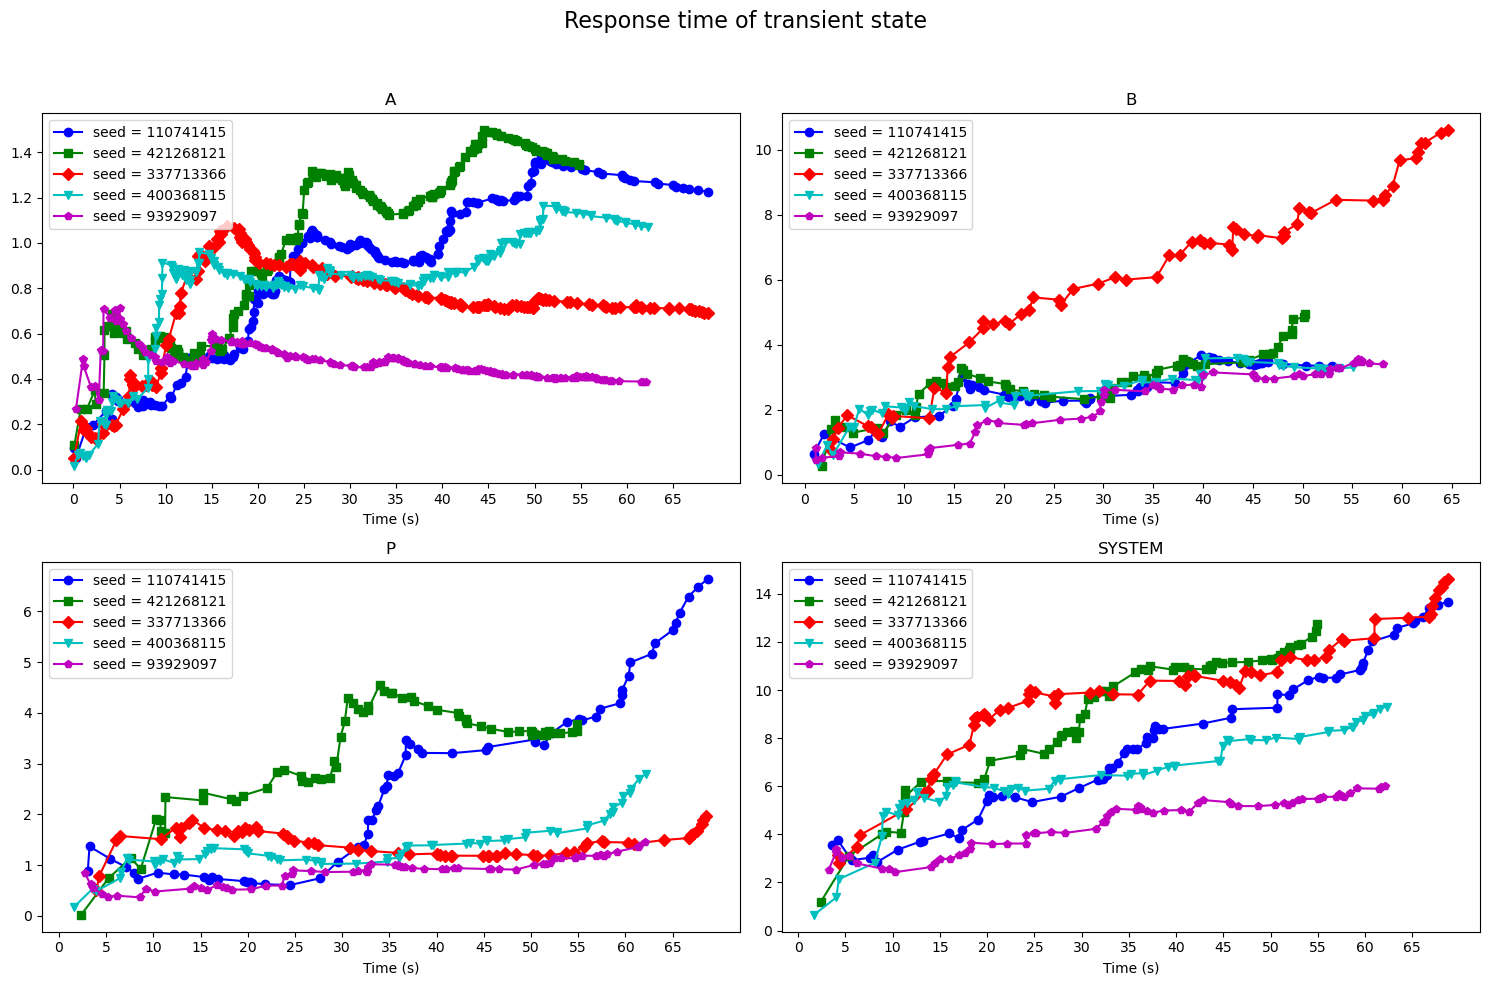
\includegraphics[width=0.8\linewidth]{figs/appendices/transient/obj2-transient-rtime.png}
        \caption{Senza valore analitico}
        \label{fig:obj2_transient_simulation}
        \end{subfigure} 
    \begin{subfigure}{\linewidth}
        \centering
        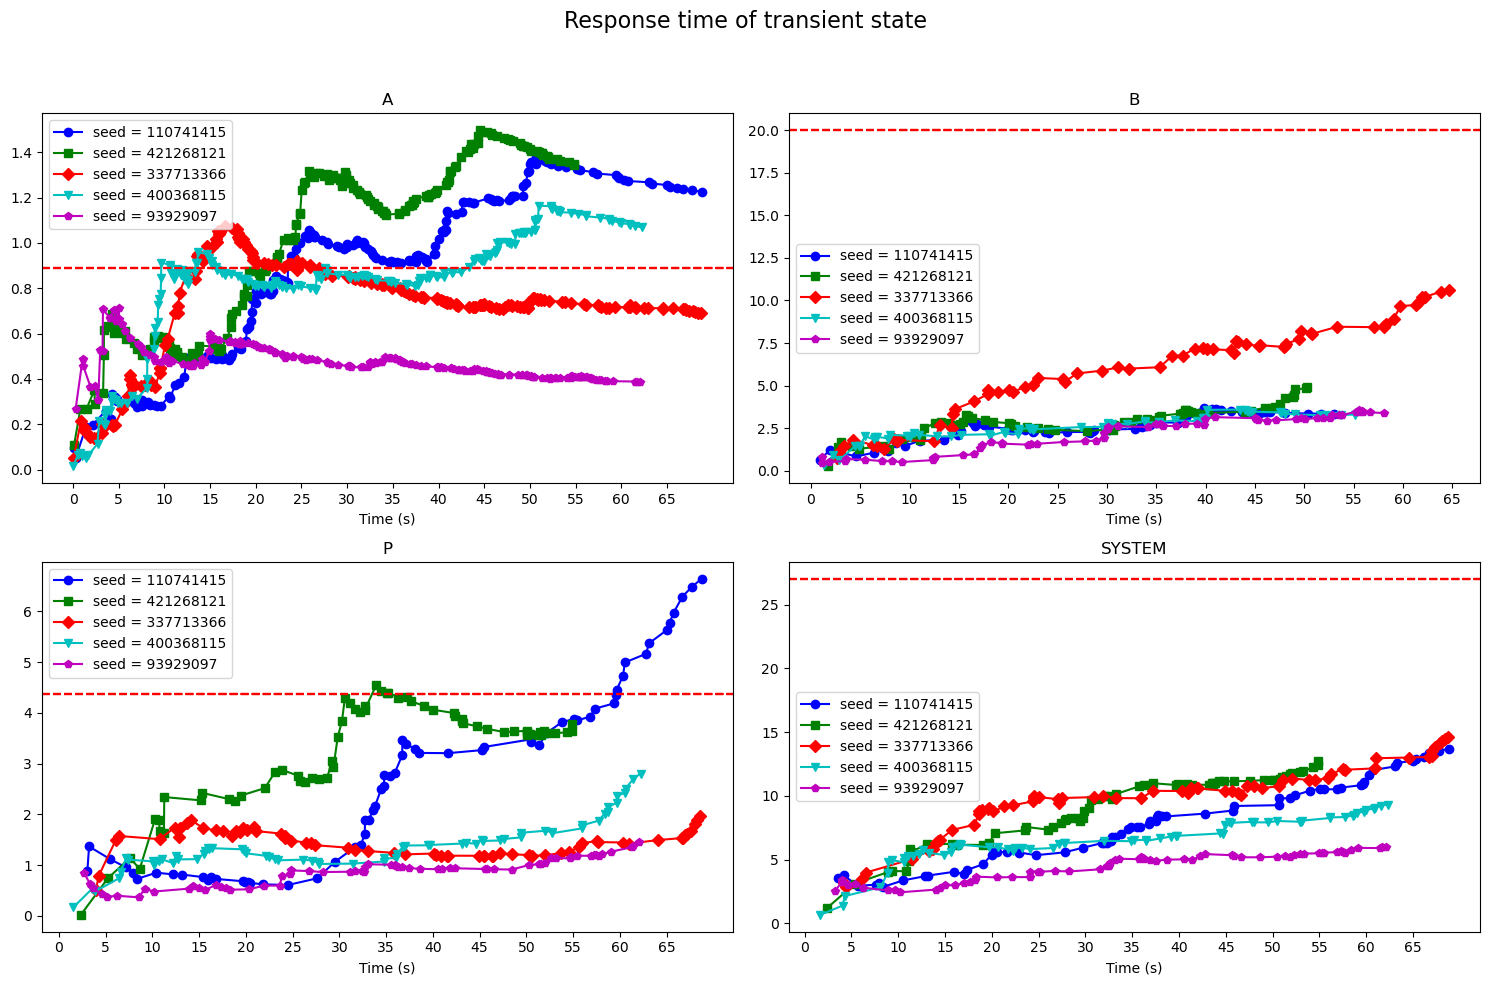
\includegraphics[width=0.8\linewidth]{figs/appendices/transient/obj2-transient-rtime-analitycal.png}
        \caption{Con valore analitico}
        \label{fig:obj2_transient_analitycal}
        \end{subfigure}
    \caption{Tempo di risposta per l'obiettivo 2 in funzione del tempo di simulazione nello stato transiente del sistema con un rate di arrivi 1.2$job/s$ al variare del seed.}
    \label{fig:obj2_transient}
\end{figure*}

\subsection{Obiettivo 3}

In \autoref{fig:obj3_transient} è riportato il valore del Tempo di Risposta medio al variare del tempo di simulazione e del seed iniziale, con un rate di arrivi medio di $1.4 job/s$, che in questo scenario rappresenta una situazione di instabilità del sistema e per questo non è disponibile un valore teorico di riferimento. Il tempo di risposta medio del server B sembra crescere esponenzialmente, e causa dei valori instabili del tempo di risposta medio del sistema. 

\begin{figure*}
    \centering
    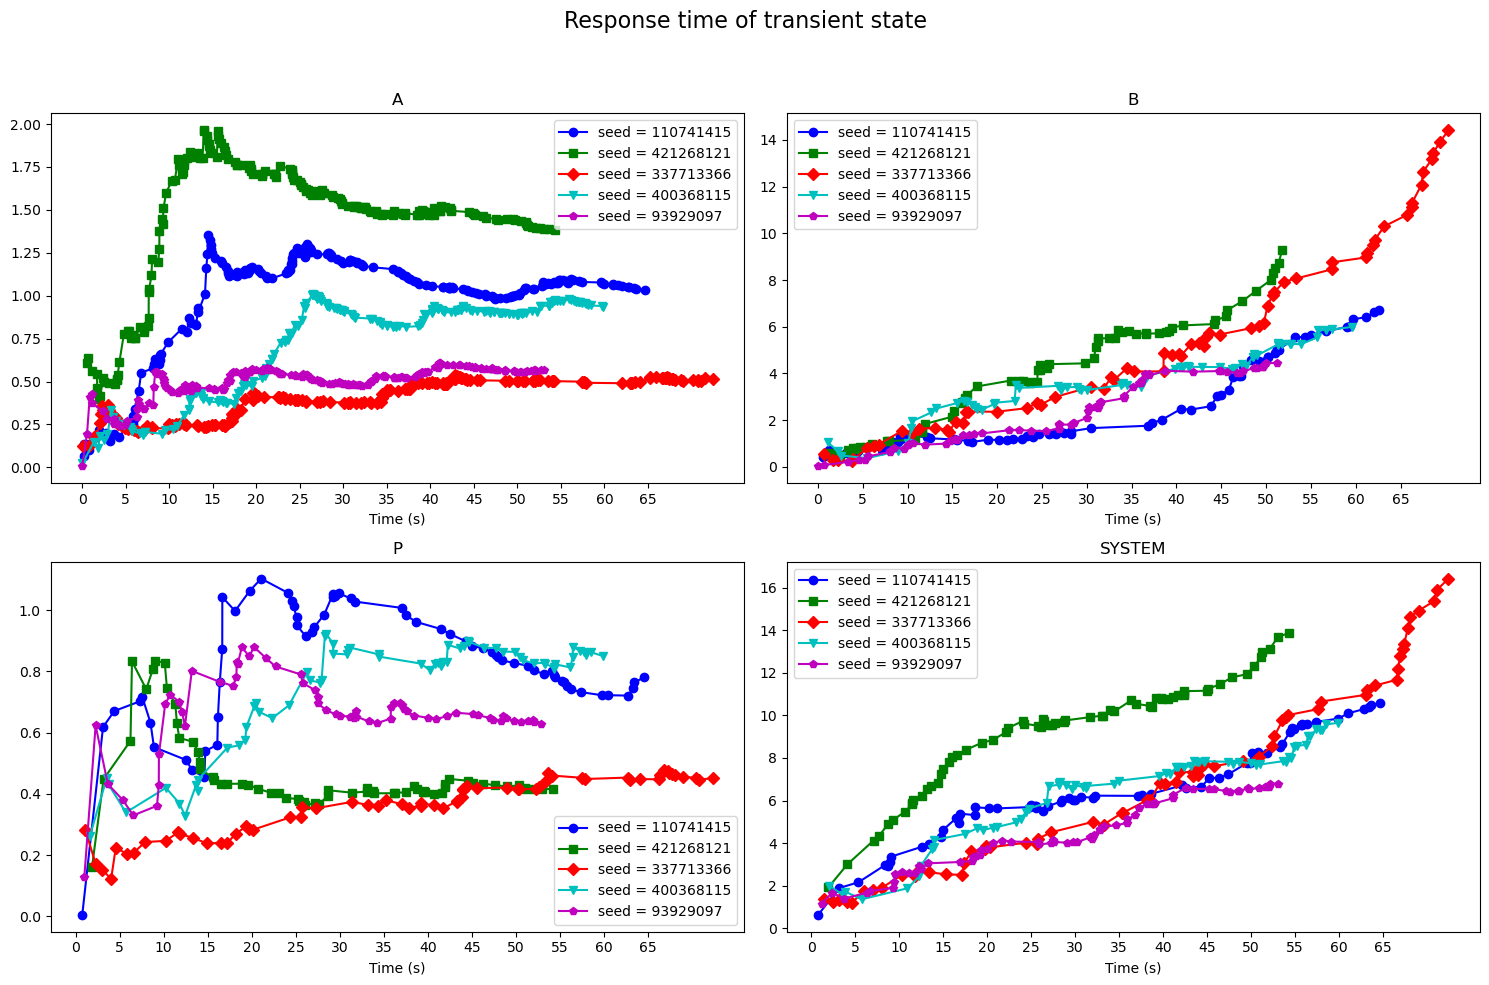
\includegraphics[width=\linewidth]{figs/appendices/transient/obj3-transient-rtime.png}
    \caption{Tempo di risposta per l'obiettivo 3 in funzione del tempo nello stato transiente del sistema con un rate di arrivi 1.4$job/s$ al variare del seed usato per la simulazione}
    \label{fig:obj3_transient}
\end{figure*}

\subsection{Obiettivo 4}

In \autoref{fig:obj4_04_transient} e \autoref{fig:obj4_065_transient} è riportato il valore del Tempo di Risposta medio al variare del tempo di simulazione e del seed iniziale, con un rate di arrivi medio di $1.4 job/s$, rispettivamente con un tempo di servizio medio per il server B di $0.4$ e $0.65s$. Sebbene entrambi i casi sembrino mostrare situazioni di stabilità, il caso con $0.65s$ sembra avere ragionevolmente valori piu alti. La \autoref{fig:obj4_065_transient_analitycal} sembra mostrare un avvicinamento maggiore ai valori teorici rispetto a \autoref{fig:obj4_04_transient_analitycal}.

\begin{figure*}
    \centering
    \begin{subfigure}{\linewidth}
        \centering
        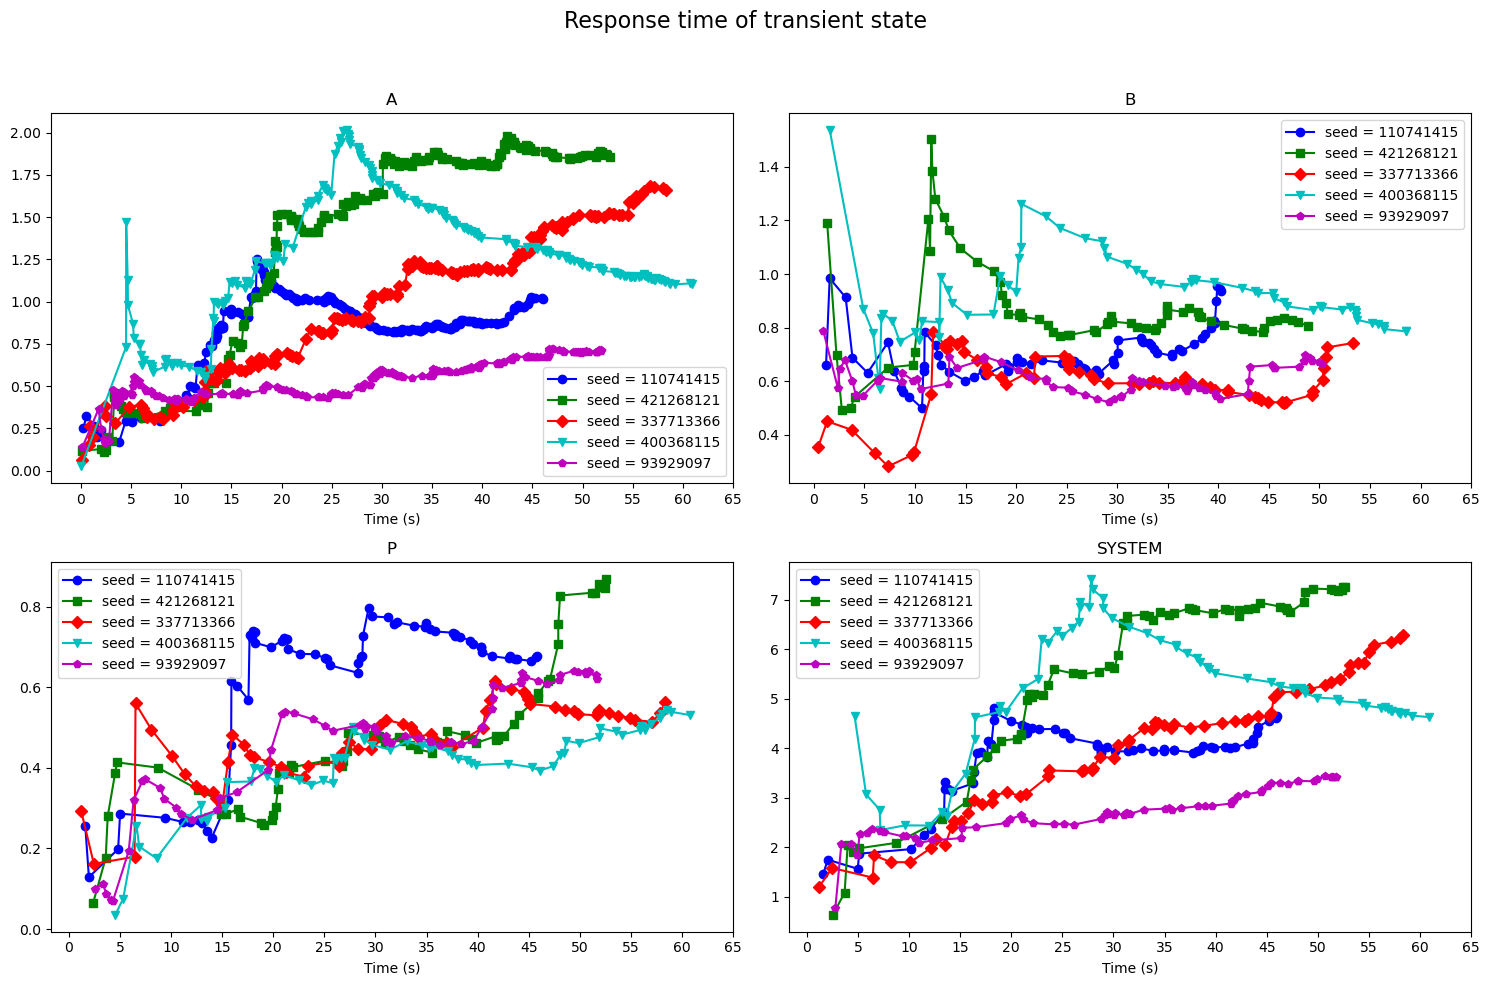
\includegraphics[width=0.8\linewidth]{figs/appendices/transient/obj4_04-transient-rtime.png}
        \caption{Senza valore analitico}
        \label{fig:obj4_04_transient_simulation}
        \end{subfigure} 
    \begin{subfigure}{\linewidth}
        \centering
        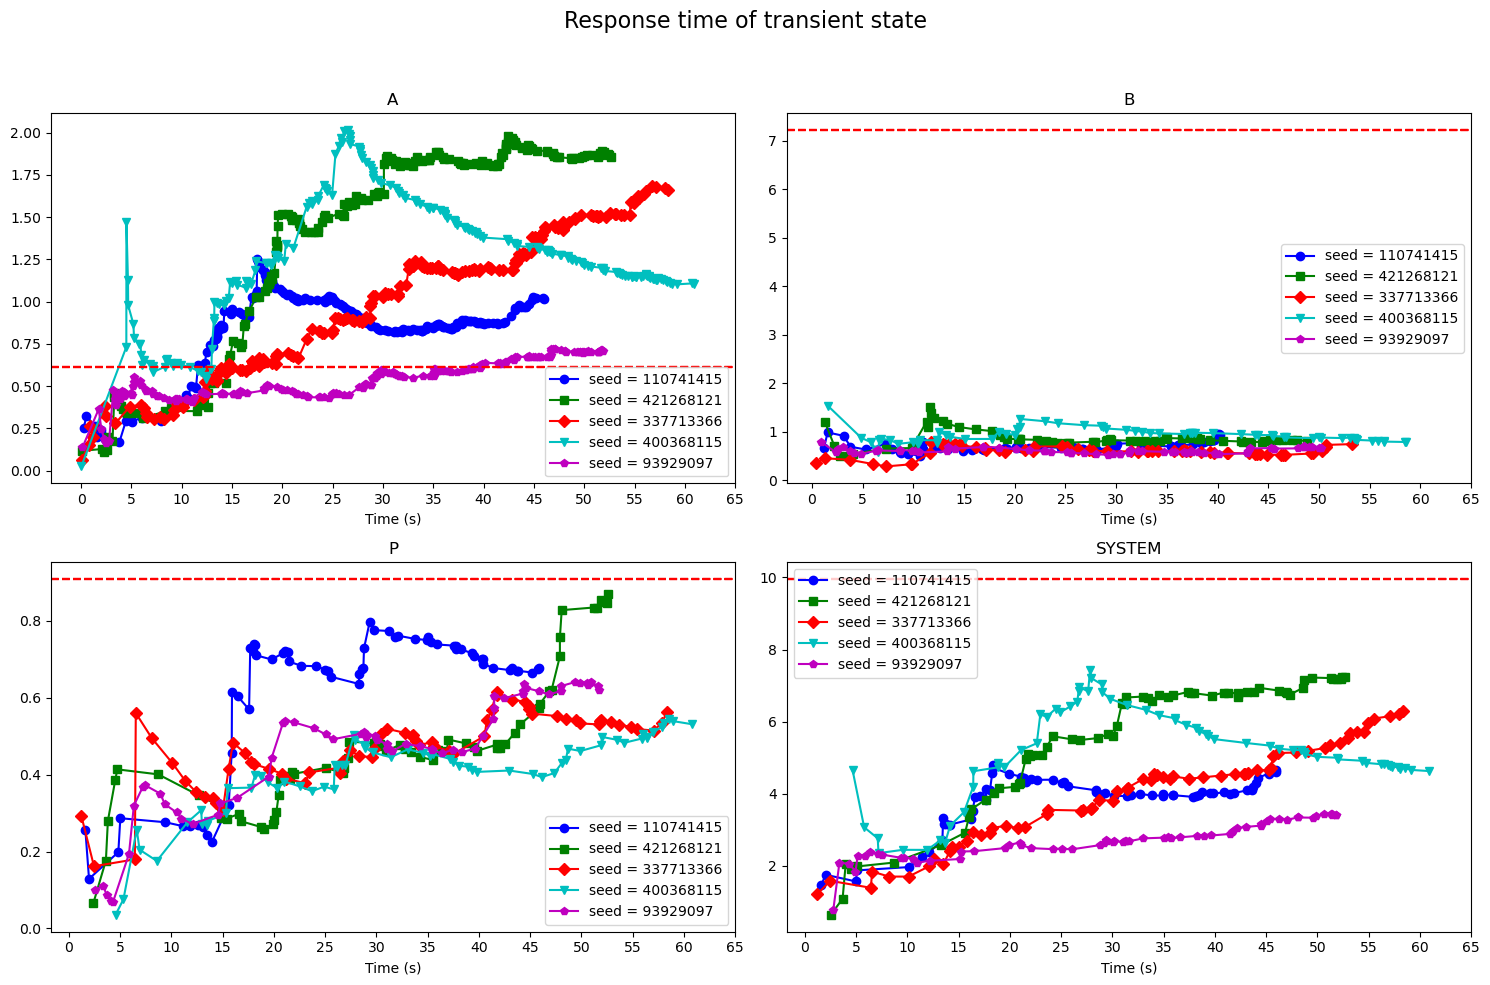
\includegraphics[width=0.8\linewidth]{figs/appendices/transient/obj4_04-transient-rtime-analitycal.png}
        \caption{Con valore analitico}
        \label{fig:obj4_04_transient_analitycal}
        \end{subfigure}
    \caption{Tempo di risposta per l'obiettivo 4 (con il server B con tempi di servizio 0.4s) in funzione del tempo di simulazione nello stato transiente del sistema con un rate di arrivi 1.4$job/s$ al variare del seed.}
    \label{fig:obj4_04_transient}
\end{figure*}

\begin{figure*}
    \centering
    \begin{subfigure}{\linewidth}
        \centering
        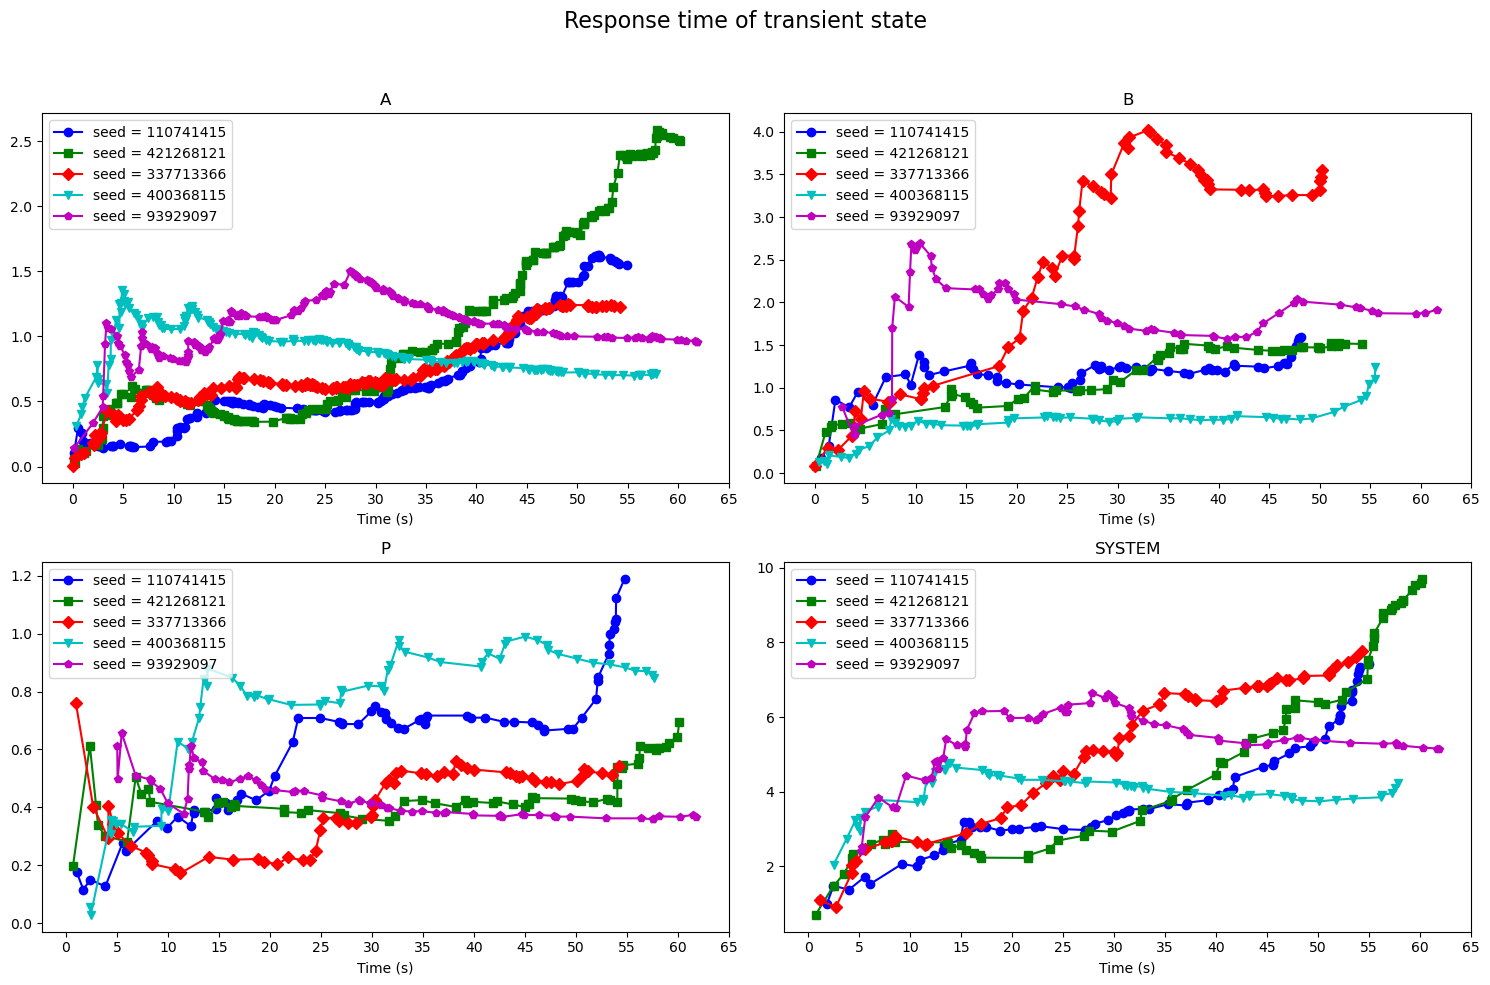
\includegraphics[width=0.8\linewidth]{figs/appendices/transient/obj4_065-transient-rtime.png}
        \caption{Senza valore analitico}
        \label{fig:obj4_065_transient_simulation}
        \end{subfigure} 
    \begin{subfigure}{\linewidth}
        \centering
        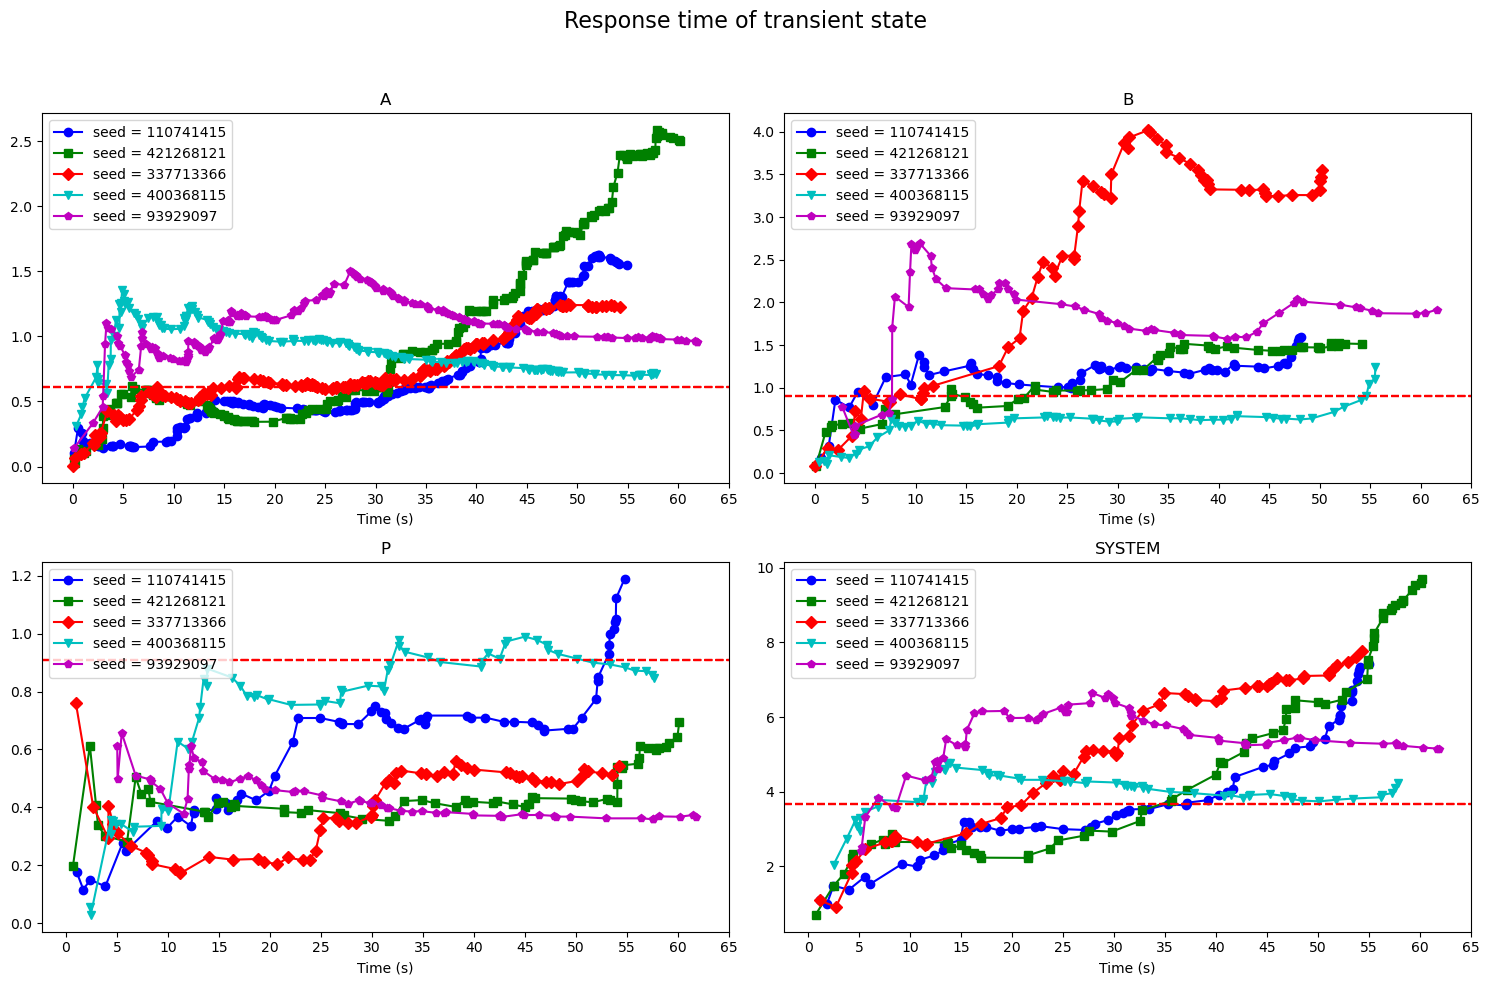
\includegraphics[width=0.8\linewidth]{figs/appendices/transient/obj4_065-transient-rtime-analitycal.png}
        \caption{Con valore analitico}
        \label{fig:obj4_065_transient_analitycal}
        \end{subfigure}
    \caption{Tempo di risposta per l'obiettivo 4 (con il server B con tempi di servizio 0.65s) in funzione del tempo di simulazione nello stato transiente del sistema con un rate di arrivi 1.4$job/s$ al variare del seed.}
    \label{fig:obj4_065_transient}
\end{figure*}



\end{document}
\endinput
